% ---------------------------------------------------------------------------
% ---------------------------------------------------------------------------
% Modelo LaTex para preparação do documento final de Dissertação de Mestrado
% O modelo está em conformidade com ABNT NBR 14724:2011: 
% Programa de Pós-Graduação em Ciência da Computação
% Universidade Federal do Piauí
% Versão: v0.9
% --------------------------------------------------------------------------- 
% ---------------------------------------------------------------------------

\documentclass[
	% -- opções da classe memoir --
	12pt,					% tamanho da fonte
	%openright,				% capítulos começam em pág ímpar (insere página vazia caso preciso)
	openany,				% capítulos começam  qualquer pág (não insere página vazia caso preciso)
	twoside,					% para impressão em verso e anverso. Oposto a oneside
	a4paper,					% tamanho do papel. 
% -- opções da classe abntex2 --       
	%chapter=TITLE,			% títulos de capítulos convertidos em letras maiúsculas
	%section=TITLE,			% títulos de seções convertidos em letras maiúsculas
	%subsection=TITLE,		% títulos de subseções convertidos em letras maiúsculas
	%subsubsection=TITLE,	% títulos de subsubseções convertidos em letras maiúsculas
	% -- opções do pacote babel --
	english,					% idioma adicional para hifenização
	%french,					% idioma adicional para hifenização
	%spanish,				% idioma adicional para hifenização
	brazil					% o último idioma é o principal do documento
	]{abntex2}

% ---------------------
% Pacotes OBRIGATÓRIOS
% ---------------------
\usepackage{lmodern}				% Usa a fonte Latin Modern			
\usepackage[T1]{fontenc}			% Selecao de codigos de fonte.
\usepackage[utf8]{inputenc}		% Codificacao do documento (conversão automática dos acentos)
\usepackage{lastpage}			% Usado pela Ficha catalográfica
\usepackage{indentfirst}			% Indenta o primeiro parágrafo de cada seção.
\usepackage{color}				% Controle das cores
\usepackage{graphicx,graphicx}	% Inclusão de gráficos
\usepackage{epsfig,subfig}		% Inclusão de figuras
\usepackage{microtype} 			% Melhorias de justificação
% ---------------------
		
% ---------------------
% Pacotes ADICIONAIS
% ---------------------
\usepackage{lipsum}						% Geração de dummy text
\usepackage{amsmath,amssymb,mathrsfs}	% Comandos matemáticos avançados 
\usepackage{setspace}  					% Para permitir espaçamento simples, 1 1/2 e duplo
\usepackage{verbatim}					% Para poder usar o ambiente "comment"
\usepackage{tabularx} 					% Para poder ter tabelas com colunas de largura auto-ajustável
\usepackage{afterpage} 					% Para executar um comando depois do fim da página corrente
\usepackage{url} 						% Para formatar URLs (endereços da Web)
\usepackage[ruled,vlined]{algorithm2e}                % Escrever algoritmo = tarcisio
\usepackage{wasysym}
\usepackage{longtable}
\usepackage{multirow}
\usepackage[table,xcdraw]{xcolor}
\usepackage{epigraph}               % adicionado por tarciisio
% ---------------------

% ---------------------
% Pacotes de CITAÇÕES
% ---------------------
\usepackage[brazilian,hyperpageref]{backref}	% Paginas com as citações na bibl
%\usepackage[alf]{abntex2cite}				% Citações padrão ABNT (alfa)
%\usepackage[num]{abntex2cite}				% Citações padrão ABNT (numericas)
\usepackage[alf,abnt-etal-cite=2 ]{abntex2cite} % acrescentado por tarcisio
% ---------------------

% Configurações de CITAÇÕES para abntex2
% --- 
% CONFIGURAÇÕES DE PACOTES
% --- 

% ---
% Configurações do pacote backref
% Usado sem a opção hyperpageref de backref
\renewcommand{\backrefpagesname}{Citado na(s) página(s):~}
% Texto padrão antes do número das páginas
\renewcommand{\backref}{}
% Define os textos da citação
\renewcommand*{\backrefalt}[4]{
	\ifcase #1 %
		Nenhuma citação no texto.%
	\or
		Citado na página #2.%
	\else
		Citado #1 vezes nas páginas #2.%
	\fi}%
% ---

% Inclusão de dados para CAPA e FOLHA DE ROSTO (título, autor, orientador, etc.)
% ---
% Informações de dados para CAPA e FOLHA DE ROSTO
% ---
\titulo{Uso de Algoritmos Aprendizado de Máquina Supervisionado para Rotulação de Dados}
\autor{Tarcísio Franco Jaime}
\local{Teresina-PI}
\data{Junho de 2018}
\orientador{Vinicius Ponte Machado}
%\coorientador{Fulano Coorientador}
\instituicao{%
  Universidade Federal do Piauí -- UFPI
  \par
  Centro de Ciências da Natureza
  \par
  Programa de Pós-Graduação em Ciência da Computação}
\tipotrabalho{Qualificação (Mestrado)}
% O preambulo deve conter o tipo do trabalho, o objetivo,
% o nome da instituição e a área de concentração
\preambulo{\textbf{Qualificação de Mestrado} apresentada ao Programa de Pós-Graduação em Ciência da Computação da UFPI (área de concentração: Sistemas de Computação), como parte dos requisitos necessários para a obtenção do Título de Mestre em Ciência da Computação.}
% ---


% Inclui Configurações de aparência do PDF Final
%  Configurações de aparência do PDF final
% NÃO ALTERAR!!!

% alterando o aspecto da cor azul
\definecolor{blue}{RGB}{41,5,195}

% informações do PDF
\makeatletter
\hypersetup{
     	%pagebackref=true,
		pdftitle={\@title}, 
		pdfauthor={\@author},
    		pdfsubject={\imprimirpreambulo},
	    pdfcreator={LaTeX with abnTeX2},
		pdfkeywords={abnt}{latex}{abntex}{abntex2}{trabalho acadêmico}, 
		colorlinks=true,       		% false: boxed links; true: colored links
    		linkcolor=blue,          	% color of internal links
    		citecolor=blue,        		% color of links to bibliography
    		filecolor=magenta,      		% color of file links
		urlcolor=blue,
		bookmarksdepth=4
} 
\makeatother
% --- 

% O tamanho da identação do parágrafo é dado por:
\setlength{\parindent}{1.3cm}

% Controle do espaçamento entre um parágrafo e outro:
\setlength{\parskip}{0.2cm}  % tente também \onelineskip

% ---------------------
% Compila o indice
% ---------------------
\makeindex
% ---------------------

%%%%%%%%%%%%%%%%%%%%%%%%%%%
%%  INICIO DO DOCUMENTO  %%
%%%%%%%%%%%%%%%%%%%%%%%%%%%
\begin{document}

% Retira espaço extra obsoleto entre as frases.
\frenchspacing

% ----------------------------------------------------------
% ELEMENTOS PRÉ-TEXTUAIS (Capa, Resumo, Abstract, etc.)
% ----------------------------------------------------------
\pretextual

% Capa
% ---
% Impressão da Capa
% ---
  \begin{capa}%
    \begin{figure}[h!]%
        \centering%
        
\includegraphics[scale=0.2]{figs/logo.pdf}%
      \end{figure}%
    \center
	\ABNTEXchapterfont\large{Universidade Federal do Piau\'i \\ Centro de Ci\^encias da Natureza \\ Programa de P\'os-Gradua\c{c}\~ao em Ci\^encia da Computa\c{c}\~ao}
	%\vspace{1.5cm}

    \vfill
    \ABNTEXchapterfont\bfseries\LARGE\imprimirtitulo
    \vfill

	%\vfill
	\ABNTEXchapterfont\large\imprimirautor
	\vfill
%
	Número de Ordem PPGCC: M001
	
    \large\imprimirlocal, \large\imprimirdata

    \vspace*{1cm}
  \end{capa}
% ---

% Folha de rosto (o * indica que haverá a ficha bibliográfica)
\imprimirfolhaderosto*

% Imprimir Ficha Catalografica
% ---
% Ficha Catalográfica
% ---
% Isto é um exemplo de Ficha Catalográfica, ou ``Dados internacionais de
% catalogação-na-publicação''. Você pode utilizar este modelo como referência. 
% Porém, provavelmente a biblioteca da sua universidade lhe fornecerá um PDF
% com a ficha catalográfica definitiva após a defesa do trabalho. Quando estiver
% com o documento, salve-o como PDF no diretório do seu projeto e substitua todo
% o conteúdo de implementação deste arquivo pelo comando abaixo:
%
% \begin{fichacatalografica}
%     \includepdf{fig_ficha_catalografica.pdf}
% \end{fichacatalografica}
\begin{fichacatalografica}
	\vspace*{\fill}					% Posição vertical
	\hrule							% Linha horizontal
	\begin{center}					% Minipage Centralizado
	\begin{minipage}[c]{12.5cm}		% Largura
	
	\imprimirautor
	
	\hspace{0.5cm} \imprimirtitulo  / \imprimirautor. --
	\imprimirlocal, \imprimirdata-
	
	\hspace{0.5cm} \pageref{LastPage} p. : il. \\
	
	\hspace{0.5cm} \imprimirorientadorRotulo~\imprimirorientador\\
	
	\hspace{0.5cm}
	\parbox[t]{\textwidth}{\imprimirtipotrabalho~--~\imprimirinstituicao,
	\imprimirdata.}\\
	
	\hspace{0.5cm}
		1. Rotulação.
		2. Algoritmos Supervisionados.
		3. CART.
		4. Naive Bayes.
		I. Dr. Vinicius Ponte Machado.
		II. Universidade Federal do Piauí.
		III. \imprimirtitulo.\\ 			
	
	\hspace{8.75cm} CDU 02:141:005.7\\
	
	\end{minipage}
	\end{center}
	\hrule
\end{fichacatalografica}
% ---


% Inserir Folha de Aprovação
% ---
% Assinaturas
% ---
% Isto é um exemplo de Folha de aprovação, elemento obrigatório da NBR
% 14724/2011 (seção 4.2.1.3). Você pode utilizar este modelo até a aprovação
% do trabalho. Após isso, substitua todo o conteúdo deste arquivo por uma
% imagem da página assinada pela banca com o comando abaixo:
%
% \includepdf{folhadeaprovacao_final.pdf}
%
\begin{folhadeaprovacao}

  \begin{center}
    {\ABNTEXchapterfont\large\imprimirautor}

    \vspace*{\fill}\vspace*{\fill}
    \begin{center}
      \ABNTEXchapterfont\bfseries\Large\imprimirtitulo
    \end{center}
    \vspace*{\fill}
    
    \hspace{.45\textwidth}
    \begin{minipage}{.5\textwidth}
        \imprimirpreambulo
    \end{minipage}%
    \vspace*{\fill}
   \end{center}
        
   Trabalho aprovado. \imprimirlocal, 01 de janeiro de 2018:

   \assinatura{\textbf{\imprimirorientador} \\ Orientador} 
   \assinatura{\textbf{\imprimircoorientador} \\ Co-Orientador} 
   \assinatura{\textbf{Professor} \\ Convidado 1}
   \assinatura{\textbf{Professor} \\ Convidado 2}
   \assinatura{\textbf{Professor} \\ Convidado 3}
      
   \begin{center}
    \vspace*{0.5cm}
    {\large\imprimirlocal}
    \par
    {\large\imprimirdata}
    \vspace*{1cm}
  \end{center}
  
\end{folhadeaprovacao}
% ---


% Dedicatória
%% ---
% Dedicatória
% ---
\begin{dedicatoria}
   \vspace*{\fill}
   \centering
   \noindent
   \textit{ Aos meus pais XXXXXXXX e YYYYYYY, \\ por sempre estarem comigo em todos os momentos.} \vspace*{\fill}
\end{dedicatoria}
% ---

% Agradecimentos
%% ---
% Agradecimentos
% ---
\begin{agradecimentos}

Agradeço a Deus.

Agradeço aos meus pais, XXXXX e YYYYY, por ...

Aos meus irmãos, por.....

Agradeço ao meu orientador, XXXXXXXXX, por todos os conselhos, pela paciência e ajuda nesse período.

Aos meus amigos ...

Aos professores ...

À XXXXXX pelo apoio financeiro para realização deste trabalho de pesquisa.

\end{agradecimentos}
%% ---

% Epígrafe
%% ---
% Epígrafe
% ---
\begin{epigrafe}
    \vspace*{\fill}
	\begin{flushright}
		\textit{``Não sei o que, \\
		          não sei o que,\\
                  não sei o que lá.''\\
		          (Autor Desconhecido)}
	\end{flushright}
\end{epigrafe}
% ---

% Resumo e Abstract
% ---
% RESUMOS
% ---

% RESUMO em português
\setlength{\absparsep}{18pt} % ajusta o espaçamento dos parágrafos do resumo
\begin{resumo}
Frente ao aumento do tráfego de dados em consequência de novas tecnologias, como também a necessidade de mais equipamentos  conectados à rede passíveis de processamento de dados, cada vez mais algoritmos de aprendizado de máquina estão sendo estudados para  extraírem dados relevantes de grandes volumes de dados. A partir desse problema de interpretação, em grandes volumes de dados, tem-se um grau de dificuldade diretamente proporcional ao crescimeto desse volume. É nesse tema  onde este trabalho atua, no entendimento dos grupos que são formados e não na criação dos mesmos. Diante o entendimento desses grupos esta pesquisa realiza de forma empírica, ou seja, através de experimentos e testes, a identificação de atributos mais significativos no grupo, junto com faixa de valores que mais se repetem a ponto de representá-lo (rotulação).  Dessa forma para a realização da rotulação de grupos de dados a proposta desta pesquisa é utilizar dois algoritmos supervisionados, cada um, com paradigmas diferentes: Naive Bayes (estatístico) e CART (simbólico). E a partir dos testes demonstrar que a rotulação é capaz de representar o grupo. Nos resultados obtemos uma acurácia acima de 70\% de acerto dos valores representados pelo rótulo escolhido.

% Segundo a ABNT, o resumo deve ressaltar o  objetivo, o método, os resultados e as conclusões do documento. A ordem e a extensão  destes itens dependem do tipo de resumo (informativo ou indicativo) e do  tratamento que cada item recebe no documento original. O resumo deve ser  precedido da referência do documento, com exceção do resumo inserido no  próprio documento. (\ldots) As palavras-chave devem figurar logo abaixo do  resumo, antecedidas da expressão Palavras-chave:, separadas entre si por  ponto e finalizadas também por ponto.

  \textbf{Palavras-chaves}: cluster. rotulação. aprendizado supervisionado. 
\end{resumo}

% ABSTRACT in english
\begin{resumo}[Abstract]
 \begin{otherlanguage*}{english}
   This is the english abstract.

   \vspace{\onelineskip}
 
   \noindent 
   \textbf{Keywords}:  cluster. rotulação.
 \end{otherlanguage*}
\end{resumo}


% Lista de ilustrações
\pdfbookmark[0]{\listfigurename}{lof}
\listoffigures*
\cleardoublepage

% Lista de tabelas
\pdfbookmark[0]{\listtablename}{lot}
\listoftables*
\cleardoublepage

% Lista de abreviaturas e siglas
\begin{siglas}
  \item [ANN] Artificial Neural Networks
  \item[EWD] Equal Width Discretization
  \item[EFD] Equal Frequence Discretization
  \item[CART] Classification and Regression Trees
  \item[RNA] Redes Neurais Artificiais
  \item[GP] Grau de Pertinência
  \item[GS] Grau de Seleção
  \item[IGS] Incremento do Grau de Seleção
  \item[SVM] Support Vector Machine
  \item[TEDA] Typicality and Eccentricity Data Analytics
\end{siglas}

% Lista de símbolos
%\begin{simbolos}
%\item[$ \Gamma $] Letra grega Gama
%  \item[$ \Lambda $] Lambda
%  \item[$ \zeta $] Letra grega minúscula zeta
%  \item[$ \in $] Pertence
%\end{simbolos}

% Inserir o SUMÁRIO
\pdfbookmark[0]{\contentsname}{toc}
\tableofcontents*
\cleardoublepage

% ----------------------------------------------------------
% ELEMENTOS TEXTUAIS (Capítulos)
% ----------------------------------------------------------
\textual
% Elementos textuais com numeração arábica
\pagenumbering{arabic}
% Reinicia a contagem do número de páginas
\setcounter{page}{1}
\newtheorem{teorema}{Definição}

% Inclui cada capitulo da Dissertação
% ----------------------------------------------------------
% Introdução 
% Capítulo sem numeração, mas presente no Sumário
% ----------------------------------------------------------

%\chapter*[Introdução]{Introdução}
%\addcontentsline{toc}{chapter}{Introdução}

% ----------------------------------------------------------
% Introdução 
% Capítulo com numeração, mas presente no Sumário
% ----------------------------------------------------------
\chapter{Introdução} \label{cap:introd}

Com a popularização da internet e mídias sociais, cada vez mais dados são processados, transportados e produzidos. E hoje, termo como, Big Data, faz parte do cotidiano de empresas e pessoas. De acordo com o autor \citeonline{Montgomery2013} Big Data são os dados que excedem a capacidade de sistemas de banco de dados. É nesse cenário, com grandes volumes de dados, que não só a formação de grupos ganha importância, mas também a compreensão dos mesmos, pois a interpretação dos grupos fornecerá informações úteis para análises desses clusters.

Agrupamento de dados, ou clustering, é o termo que se usa para identificar dois ou mais objetos pertencentes ao mesmo grupo que compartilham um conceito em comum \cite{Kumar2013}. Cluster é um termo bastante pesquisado no aprendizado não-supervisionado (subárea do aprendizado de máquina) e  aplicada em vários contextos como segmentação de imagens, recuperação de informação e reconhecimento de objetos. Os algoritmos de agrupamento, conforme \citeonline{Kumar2013}, são aplicados em diferentes campos: Biologia (classificação de plantas e animais), Marketing (encontrar grupos de clientes com comportamentos semelhantes), planejamento de cidades (identificação de casas de acordo com seu tipo, valor e localização geográfica), entre outros.

O grau de escalabilidade dos dados gradativamente aumenta no decorrer dos anos, e embora os estudos sobre o problema de agrupamento de dados estejam avançados, fica cada vez mais complexo o entendimento dos clusters formados, pela razão do número crescentes de grupos criados. Quanto maiores são os números de grupos produzidos mais  difícil são suas interpretações. 

Diante desse contexto é que se extrai a temática desta proposta de mestrado qual seja - ''Rotulação automática de grupos através de algoritimos supervisionados baseados em árvores e estatísticos'' - o estudo em questão dedica-se na aplicabilidade de dois algoritimos supervisionados, com paradigmas diferentes e bases de dados distintas, a fim de  definir a tupla atributo/valor de maior importância nos clusters, determinando um significado para estes clusters (rotulação).


A formação do problema desta pesquisa nasce a partir do trabalho realizado por \citeonline{LOPES2014},  que se dedicou a estudar a possibilidade de realização de  rotulação automática de grupos utilizando  algoritmo não-supervisionado (K-means) para formação de grupos e algoritmo supervisionado (Redes Neurais) para a rotulação. Assim, partindo deste estudo já realizado, este trabalho questiona-se:  É possível realizar rotulação de grupos de dados a partir de outros algoritmos supervisionados não testados, em específico Naive Bayes e CART?

Acredita-se que o resultado de tal problemática será positivo, considerando que os algoritmos Naives Bayes e CART também são categorizados como supervisionados. Além disso, é necessário mensurar ainda, a acurácia de cada resultado através do percentual de acertos dos atributos que são representados pelos rótulos gerados. Assim, se for possível demonstrar que a acurácia é de pelo menos 60\% ficará então comprovada a possibilidade de se fazer rotulação dos grupos de dados utilizando os algoritimos supervisionados Naive Bayes e CART, pois percentuais menores do rótulo não representariam o grupo. Importante destacar, que este trabalho não se preocupa em criar grupos, mas dar maior relevância à rotulação dos mesmos, isto é, compreender os grupos de dados já formados.

O termo rotulação, neste trabalho, segue a definição conforme \citeonline{LOPES2014}: 

%\newtheorem{teorema}{Definição}
    \begin{teorema}
    Dado um conjunto de clusters ${C=\{c_1,...,c_k | K \geqslant 1\} }$, de modo que cada cluster contém um conjunto de elementos ${c_i=\{\vec{e}_1,..,\vec{e}_{n^{(c_i)}}|n^{(c_i)} \geqslant 1 \}}$ que podem ser representados por um vetor de atributos definidos em ${\mathbb{R}^m }$ e expresso por ${ \vec{e}^{c_i}=(a_1,..,a_m)  }$ e ainda que  com ${ c_i \cap c_{i'}=\{\emptyset\} }$ com ${ 1 \leqslant i, i \leqslant K  }$ e ${ i \neq i' }$; o objetivo consite em apresentar um conjunto de rótulos ${ R=\{ r_{c1},...,r_{ck} \} }$, no qual cada rótulo específico é dados por um conjunto de pares de valores, atributo e seu respectivo intervalo, ${ r_{ci}=\{ (a_1,[p_1,q_1]),...,(a_{m^{(c_i)}}, ]p_{m^{(c_i)}},q_{m^{(c_i)}}]) \} }$ capaz de melhor expressar o cluster ${c_i}$ associado.
        %\footnotemark 
        %\footnotetext{Definição retirada de \cite{LOPES2014}}
        \begin{itemize}[noitemsep]
            \item ${K}$ é o número de clusters;
            \item ${c_i}$ é o i-ésimo cluster qualquer;
            \item ${n^{c_i}}$ é o número de elementos do cluster ${c_i}$;
            \item ${\vec{e}_{n^{(c_i)}}}$ se refere ao j-ésimo elemento pertencente ao cluster ${c_i}$;
            \item ${m}$ é a dimensão do problema;
            \item ${r_{c_i}}$ é o rótulo referente ao cluster ${c_i}$;
            \item ${]p_{m^{(c_i)}},q_{m^{(c_i)}}]}$ representa o intervalo de valores do atributo ${a_{m^{(c_i)}} }$, onde ${ p_{m^{(c_i)}} }$  é o limite inferior e ${ q_{m^{(c_i)}} }$ é o limite superior;
            \item ${m}$ é a dimensão do problema;
        \end{itemize}
    \label{teo:lopes:problema}
    \end{teorema}

Em um exemplo, no qual a base de dados possui classes já definidas: macho, fêmea ou raça X, Y, Z, etc. E que ao criar esses grupos sabe-se que existe uma correlação das características dos grupos, acabando por não deixar visível qual característica se apresenta mais significativa dentro desses grupos. Tem-se na rotulação a intenção de definir algum significado para estes grupos, gerando um tipo de rótulo, ${ R=\{ r_{c1},...,r_{ck} \} }$, para melhor expressar o cluster ${c_i}$ associado (Definição \ref{teo:lopes:problema}).

Tecnicamente a informação do rótulo aplicada no cluster pode ajudar na tomada de decisão em algum contexto. A exemplo disso, supõe-se uma situação empregada na área urbana, onde pessoas circulam na cidade e imagina-se que os dados de controle de seus celulares estão sendo capturados pelas células das torres, e gravados em uma base de dados pelas operadoras. Uma vez em posse desses dados, são criados clusters podendo ser aplicado rotulação nestes grupos. E através dos rótulos pode-se personalizar alguns serviços para esses grupos já formados. 

Seguindo o exemplo dos dados capturados do celular, caso o rótulo (${r_{c_i}}$) de um cluster (${c_i}$) fosse o  atributo localização, e os valores  desse atributo escolhido para compor o rótulo, fossem as coordenadas geográficas, o qual definiriam o tipo de localização. Logo percebe-se que os participantes desse grupo possuem característica de frequentar alguma localização em comum. A interpretação deste rótulo poderá implicar em uma tomada de decisão personalizada para este grupo, objetivando otimizar um problema.

O trabalho em questão tem como objetivo principal demonstrar a  possibilidade de fazer rotulação de dados, em grupos já formados, utilizando dois algoritimos supervisionados distintos com paradigmas diferentes. Sendo este um algoritmo com paradigma estatístico - Naive Bayes -  e outro com paradigma simbólico - Classification And Regression Tree (CART).
 
Para alcançar tal objetivo é necessário ???? (falar do objetivo de cada capítulo)foi estruturada mediante a codificação por intermédio de uma linguagem de natureza técnica, onde fez uso de módulos de aprendizado de máquina, atuando em bases de dados e obtendo como saída deste programa, os rótulos dos grupos. Uma vez que estes grupos já possuem informações do provedor das bases de dados de como foram criados.

Esta pesquisa é eminentemente quantitativa, pois se utiliza de algoritmos supervisionados para selecionar os atributos de maior relevância nos clusters, através de um percentual de correlação entre atributos, isto é, quanto maior esse percentual maior será a relevância desse atributo em relação aos outros. Além disso faz uma análise da base de dados de forma subjetiva para definir o número de faixas que serão divididos os valores, para realização da discretização. Uma vez escolhido o atributo de maior relevância e selecionada a faixa de valor que mais se repete nesse atributo, o resultado será o rótulo composto pela tupla: atributo mais importante e faixa selecionada. 

O trabalho será disposto em cinco capítulos já incluso  a Introdução e Conclusão, capítulos \ref{cap:introd} e \ref{cap:conclusao} respectivamente.  

O Referencial Teórico abordado no capítulo \ref{cap:refTeor} é responsável em esclarecer as tecnologias utilizadas nesta pesquisa e dividida em três seções. Inicialmente na seção \ref{cap:refTeor:sec:aprendMaq}, tem-se uma  explanação sobre aprendizado de máquina e quais os aprendizados indutivos são mais relevantes para este trabalho, ademais, a explicação dos dois algoritmos supervisionados utilizados para fazer rotulação de dados. Já na seção \ref{cap:refTeor:sec:discret} é realizado a divisão das faixas de valores de cada atributo, chamada de discretização. E logo na seção \ref{cap:refTeor:sec:trabcorrel} são apresentas pesquisas já consolidadas  referentes ao assunto de rotulação de clusters.

Na capítulo \ref{cap:ferramentas} é abordada a definição do problema da pesquisa. A partir dessa definição um modelo de resolução é definido e apresentado um fluxograma exibindo os processos a serem seguidos. Logo na seção \ref{cap:ferramentas:sec:tecnica} é demonstrado o funcionamento da técnica de correlação entre atributos. E na seção \ref{cap:ferramentas:sec:exebasemodfic} uma base de dados fictícia é utilizada para exemplificar a execução dos processos do modelo de resolução: discretização da base de dados no Processos (I), no Processo (II) é aplicado o algoritmo supervisionado e no Processo (III) o resultado da rotulação. 

No capítulo \ref{cap:resultados} os resultados são apresentados separados por cada base de dados. Sendo que em cada algoritmo testado o resultado é dividio em cluster, atributo rótulo desse cluster, faixa de valores compondo o rótulo e mais dois campos expondo o grau de relevância, em porcentagem, de cada atributo em relação aos outros, junto com o número de elementos que não são representados pelo rótulo escolhido. A partir destas informações é retirado o rótulo o qual representará o cluster.

Diante de todo o exposto fica claro que esta pesquisa além de dar continuidade a um tema específico aplicado na interpretação de agrupamento de dados, também serve como ponto de partida para outra pesquisa mais aprofundada, onde poderá esta tentar comprovar a possibilidade de fazer rotulação de dados utilizando qualquer algoritmo supervisionado.

% \section*{Motivação}\label{sec:motivacao}
% \addcontentsline{toc}{section}{Motivação}

% \lipsum[35]

% \section*{Objetivos}\label{sec:objetivos}
% \addcontentsline{toc}{section}{Objetivos}

% \lipsum[36]

% PARTE - Define a divisão do documento em partes (Não é obrigatório)
%\part{Preparação da pesquisa}
%% ---
\chapter{Uso de referências bibliográficas}
% ---

A formatação das referências bibliográficas conforme as regras da ABNT são um
dos principais objetivos do \abnTeX. Consulte os manuais
\citeonline{abntex2cite} e \citeonline{abntex2cite-alf} para obter informações
sobre como utilizar as referências bibliográficas.

%-
\subsection{Acentuação de referências bibliográficas}
%-

Normalmente não há problemas em usar caracteres acentuados em arquivos
bibliográficos (\texttt{*.bib}). Porém, como as regras da ABNT fazem uso quase
abusivo da conversão para letras maiúsculas, é preciso observar o modo como se
escreve os nomes dos autores. Na~\autoref{tabela-acentos} você encontra alguns
exemplos das conversões mais importantes. Preste atenção especial para `ç' e `í'
que devem estar envoltos em chaves. A regra geral é sempre usar a acentuação
neste modo quando houver conversão para letras maiúsculas.

\begin{table}[htbp]
\caption{Tabela de conversão de acentuação.}
\label{tabela-acentos}

\begin{center}
\begin{tabular}{ll}\hline\hline
acento & \textsf{bibtex}\\
à á ã & \verb+\`a+ \verb+\'a+ \verb+\~a+\\
í & \verb+{\'\i}+\\
ç & \verb+{\c c}+\\
\hline\hline
\end{tabular}
\end{center}
\end{table}


% ---
\section{Precisa de ajuda?}
% ---

Consulte a FAQ com perguntas frequentes e comuns no portal do \abnTeX:
\url{https://code.google.com/p/abntex2/wiki/FAQ}.

Inscreva-se no grupo de usuários \LaTeX:
\url{http://groups.google.com/group/latex-br}, tire suas dúvidas e ajude
outros usuários.



\chapter{Referencial Teórico}\label{cap:refTeor}


Para se compreender  a temática proposta  este capítulo abordará o conteúdo base deste trabalho dividido em 3 seções: Aprendizado de Máquina, Discretização e Trabalhos Correlatos. 

A aprendizagem de máquina utiliza métodos de inferências lógicas para aquisições de novos conhecimentos, e um dos tipos de inferência comentada nesta seção são os aprendizados indutivos, que dentre seus tipos terá o maior destaque  ao aprendizado supervisionado, foco dessa proposta de mestrado. ``Na aprendizagem indutiva os algoritmos podem, na melhor das hipóteses, garantir que a hipótese de saída se encaixe no conceito de destino sobre os dados de treinamento'' \cite[p.23]{Mitchell1997}.

%\epigraph{Na aprendizagem indutiva os algoritmos podem, na melhor das hipóteses, garantir que a hipótese de saída se encaixe no conceito de destino sobre os dados de treinamento. Na falta de mais informações, nossa suposição é que a melhor hipótese em relação a instâncias não vistas é a hipótese que melhor se ajusta aos dados de treinamento observados}{ \cite[p.23]{Mitchell1997}}


%No aprendizado indutivo a indução é um tipo de inferência lógica, a partir de um pequeno número de observações pode-se ter uma conclusão geral de todo o conjunto. Então, caso a pequena amostra não tenha dados suficientes ou os dados da amostra não forem relevantes, o conhecimento induzido acaba sendo prejudicado por generalizar o conhecimento adquirido, dessa amostra, para todo o grupo de dados.

Já na seção \ref{cap:refTeor:sec:discret} dissertará sobre a técnica de discretização adotada nesta pesquisa. Possuindo grande contribuição para os resultados gerados, e ganhando assim uma seção própria para explanação de como funciona essa técnica. E na seção \ref{cap:refTeor:sec:trabcorrel}, serão abordados trabalhos que possuam mesmas características desta pesquisa adicionando conhecimento ao tema.



\section{Aprendizado de Máquina}\label{cap:refTeor:sec:aprendMaq}

 A aprendizagem de máquina, diferente das metodologias tradicionais de implementação, utiliza sua experiência anterior, para melhorar suas respostas a partir de problemas em determinadas áreas. 
 
 ``Um programa de computador aprende com a experiência E em relação a alguma classe de tarefas T e medida de desempenho P, se seu desempenho em tarefas em T, conforme medido por P, melhora com a experiência E'' \cite[p. 2]{Mitchell1997}. 
 
 %\newtheorem{defaprendmaq}{Definição}
 % \begin{teorema}
 %  Um programa de computador aprende com a experiência E em relação a alguma classe de tarefas T e medida de desempenho P, se seu desempenho em tarefas em T, conforme medido por P, melhora com a experiência E
 %  \label{teo:defaprendmaq}
 % \end{teorema}
 
Para melhor explicar a citação acima, destaca-se o determinado exemplo: considerar o reconhecimento facial de uma pessoa utilizando aprendizado de máquina. Então caso fossem  inseridas várias fotos tituladas de uma certa pessoa (T) no banco de dados, e após vários exemplos (E), fotos dessa pessoa, o programa de computador seria capaz de predizer (P) se uma nova foto, ainda não inserida no banco de dados, seria dessa  determinada pessoa através de aprendizado  anterior (E), ou melhor, de fotos que foram anteriormente inseridas.

O aprendizado de máquina seriam algoritmos capazes de aprender automaticamente através de  determinados exemplos, ou comportamentos. Esse aprendizado automático preenche algumas lacunas no desenvolvimento de programas, posto que não é possível simplesmente exigir do projetista implementar melhorias em um sistema, de forma que ele esteja robusto bastante para lidar com todas as situações \cite{RusselStuart.Norvig2013}, pois seria impossível um programador antecipar todas as situações possíveis de implementação.


%Alguns motivos justificam que não é possível simplesmente exigir do projetista implementar melhorias no sistema, de forma que ele esteja robusto bastante para lidar com todas as situações \cite{RusselStuart.Norvig2013}. Um  desses motivos seria a incapacidade da antecipação de todas as situações possíveis de implementação por parte do programador. Fazendo um resumo, aprendizado de máquina seriam algoritmos capazes de aprender automaticamente através de  determinados exemplos, ou comportamentos. 

Utilizando a idéia do exemplo anterior, uma vez inserida uma foto no banco de dados e determiná-la como masculina, nesse momento, estará se fazendo uma classificação desse novo registro (nova foto). Uma vez com a base de dados classificada, pode-se utilizar algoritmos para predizer um novo registro e defini-lo como masculino ou feminino. Predizer uma determinada condição irá depender da base de dados como também do algoritmo utilizado para fazer essa classificação. Alguns  exemplos de algoritmos são:  redes neurais, árvores de decisão, Suport Vector Machine – SVM, etc. A escolha apropriada do algoritmo se dará através de métricas que avaliarão o desempenho de cada um e a melhor métrica servirá de parâmetro para a escolha do algoritmo apropriado para aquele problema de classificação de dados. 

%A partir desta síntese, tem-se uma observação. A classificação de dados no contexto de aprendizado de máquina, são compostos por dois pilares. Um, seriam os \textbf{dados} a serem classificados, e outro, o \textbf{algoritmo} que irá atuar nessa base de dados. Existem vários algoritmos como exemplo: redes neurais, árvores de decisão, Suport Vector Machine – SVM, etc. Qualquer um destes algoritmos são utilizados para encontrar um classificador. E a escolha apropriada se dará através de métricas que avaliarão o desempenho de cada um, e a melhor métrica, será o algoritmo apropriado para aquele problema de classificação de dados. 

Em aprendizado de máquina são vários as abordagens encontradas, e segundo \citeonline{Mohri2012} são eles: aprendizado supervisionado, aprendizado não-supervisionado, aprendizado semi-supervisionado, aprendizado por reforço e  muitos outros. Todavia nesta pesquisa serão comentados somente algumas abordagens de referência específicas para esse trabalho.

\subsection{Aprendizado Supervisionado}\label{cap:refTeor:ssec:aprendSup}

O aprendizado supervisionado é um método que através de uma base de dados classificada, será realizado uma predição de novos registros com base em vários desses exemplos já classificados, ou seja, é quando existem casos que possuem uma classificação disponível para determinados conjunto de dados (conjunto de treinamento), mas precisa ser previstos para outras instâncias. Os responsáveis por essas predições de novos registros são algoritmos de aprendizado supervisionados projetados para determinados fins.


O termo ``Supervisionado'' indica uma correlação entre os dados de entrada com a saída desejada (classe). Seguindo o padrão de exemplo anterior considere: uma base de dados de imagens de rostos, onde cada imagen possui uma saída representada por uma classe (masculino ou feminino). A tarefa seria criar um preditor capaz de acertar a cada novo registro se a imagem é masculina ou feminina. Seria  difícil  implementar de maneira tradicional, utilizando estruturas condicionais e laços, uma vez que são inúmeras as diferenças das faces masculinas e femininas. Embora haja uma dificuldade de distinção entre as faces, uma alternativa seria dar exemplos de rostos classificados, masculino ou feminino,  e através desses exemplos aplicar o algoritmo que automaticamente faça a máquina aprender uma regra para predizer qual sexo pertence cada rosto  \cite{Barber2011}.

Em \citeonline{RusselStuart.Norvig2013} é feito apresentação formal do funcionamento da aprendizagem supervisionada. Dado um conjunto de treinamento 
\begin{equation}
 (x_{1},y_{2}),(x_{2},y_{2}),...(x_{n},y_{n}),
 \label{eq:aprendSup}
\end{equation}
onde cada ${y_{j}} $ foi gerado por ${y=f(x)}$ desconhecida. Encontrar uma função ${h}$ que se aproxime da função ${f}$ real.

%Antes de falar dos algoritmos utilizados nesse texto, a aprendizagem supervisionada detém dois tipos de casos: regressão e classificação. A classificação, contêm variáveis com valores discretos, onde as amostras destas variáveis de saída estão na forma de categorias. Como exemplo poderia ser masculino e feminino. Já no tipo regressão, possuem valores contínuos: quantidade de água em ml, velocidade de um carro, altura de uma pessoa.

A função ${h}$ é uma hipótese onde prevê um melhor desempenho entre as hipóteses possíveis através dos conjuntos de dados, que são diferentes do conjunto de treinamento equação \ref{eq:aprendSup}.

 \begin{figure}[h!]
    \centering
    \subfloat[Ajuste polinomial de grau 6]{
        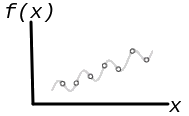
\includegraphics[scale=0.8]{figs/grafA.png}
        \label{fig:graf1:grafA} }
    \quad
    \subfloat[Hipótese linear]{
        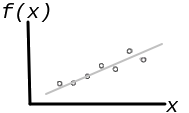
\includegraphics[scale=0.8]{figs/grafB.png}
        \label{fig:graf1:grafB} }
    
    \caption{Hipóteses ajustadas} \label{fig:graf1}
        
        %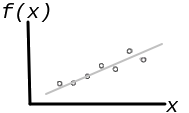
\includegraphics[scale=0.4]{figs/grafB.png}
        %\caption{Polinômio Superajustado} \label{grafB}
\end{figure}


O exemplo da figura \ref{fig:graf1:grafA} mostra uma função de grau 6 onde acontece  um sobreajuste (overfitting) no conjunto de dados de treinamento. Esse modelo acabou exibindo uma função mais complexa para atender todo o conjunto de dados do gráfico, ficando especifico para essa amostra. 

Já na figura \ref{fig:graf1:grafB} o ajuste da função se torna mais simples e mesmo o gráfico não passando por todos os pontos, acabou por generalizar melhor o conjunto de treinamento, tornando talvez, um melhor resultado da predição de novos valores. 

Em análise da figura \ref{fig:graf1} é apresentado duas hipóteses que tentam se aproximar ao máximo da função verdadeira (${h}$), que é desconhecida. Mesmo parecendo que  na figura \ref{fig:graf1:grafA} obteve-se melhor resultado, pois todos os pontos são atingidos pelo gráfico da função, este modelo acabou se ajustando muito bem na amostra de dados deixando a função ${h}$ muito específica, não retratando os dados em um mundo real. Então, apesar de parecer que a \ref{fig:graf1:grafA} por ser mais específica é a melhor função, não é a opção correta. Quanto mais  generalizado for modelo, melhor será para predizer os valores de ${y}$ para novos conjuntos de dados.

\subsubsection{Algoritmo Classification and Regression Trees  - CART}\label{cap:refTeor:sssec:cart}


Esse algoritmo constroi modelos de previsão a partir de dados de treinamento onde seus resultados podem ser reprensentados em uma árvore de decisão. A árvore de decisão é uma ferramenta que da suporte à decisão utilizando como modelo um fluxograma semelhante a uma árvore, onde a cada nó interno é feito um teste para tomada de decisão, permitindo uma abordagem do problema de forma estruturada e sistemática até chegar a uma conclusão lógica. ``Uma árvore de decisão alcança sua decisão executando uma sequência de testes'' \cite[p. 811]{RusselStuart.Norvig2013}

O algoritmo CART pode se tornar uma árvore de classificação ou também um árvore de regressão, o que irá definir seu tipo seria o atributo classe. Por exemplo, em um conjunto de dados de um paciente onde tenta prever se o mesmo possuirá câncer. A classe seria ``Terá Câncer'' ou ``Não terá Câncer''. Nesse exemplo o atributo assume duas classes.

Mas ao contrário de uma árvore de classificação que prediz uma classe, o CART também pode assumir uma árvore de regressão, onde poderá prever um valor numérico ou contínuo, como: período de tempo de internação do paciente, preço de uma cirurgia ou quantidade de água ingerida. 

No caso de não ser probabilístico o grau de confiança em seu modelo de predição será embasada em respostas semelhantes em outras circunstâncias antes analisadas. 

O CART utiliza uma técnica como partição recursiva binária. Binária porque a divisão do nó pai é sempre em dois nós filhos, e recursiva porque cada nó filho irá ser tratado posteriormente no processo como nó pai.

Inicialmente todas as amostras se concentram no nó raiz, e a partir daí é apresentado uma questão, onde a intenção é separar o nó raiz em dois grupos mais homeogêneos. O objetivo é criar uma regra que inicialmente crie grupos ou nós binários que sejam internamente mais homogêneos que o nó raiz. Dependendo da questão as amostras irão para a folha esquerda ou direita do nó raiz. O CART faz a escolha dessa divisão em função da regra Gini de Impureza\footnote{O CART pode utilizar outros critérios de divisão de dados como: entropia e critério de Twoing} \cite{breiman1984}, e o índice Gini varia de 0 a 1, definindo o grau de pureza do nó. 

\begin{equation}
Gini(S)= 1 - \sum p^2(j/t)
 \label{eq:cartGini}
\end{equation}
Onde: ${p(j/t)}$ é probabilidade a priori da classe ${j}$ se formar no nó ${t}$. E ${S}$ é um conjunto de dados que contém exemplos de n classes
%\begin{itemize}
% \item ${S}$: é um conjunto de dados que contém exemplos de n classes
% \item ${p_j}$: é uma frequência relativa da classe ${j}$ em ${S}$
%\end{itemize}

Para construção de uma árvore pode-se simplificar em três componente importantes \cite{yohannes1999classification,Raimundo2008}: 
\begin{itemize}
[noitemsep]
 \item Um conjunto de perguntas que servirá de base para fazer uma divisão;
 \item Regras de divisão para julgar o quanto é boa esta divisão;
 \item Regras para atribuir uma classe a cada nó;
\end{itemize}

Na divisão inicial será atribuído ao nó pai uma questão onde dependendo da resposta (sim ou não) os registros irão para nó filho esquerdo ou direito. Esse questionamento binário servirá dividindo o grupo em dois, para depois testar o ponto de divisão.

O CART percorrerá todos os atributos construindo uma árvore para descobrir qual melhor ponto de divisão. Uma vez testados todos os atributos é escolhido o que tiver menor grau de impureza do nó medido através do critério Gini, onde o grau de pureza do nó é mais puro, quando no grupo houver mais casos pertencente a uma única classe. Fazendo que o índice Gini seja mais alto.

Após a escolha do melhor ponto de  divisão do nó faz-se a atribuição de uma classe para o nó, onde a esolha da classe será a que mais exemplos contiver no grupo.





% 
% \IncMargin{1em}
% \begin{algorithm}[h!]
% 
% \nl $melhorGini$; \tcc{cria a variável}
% \nl $divisaoCorrente \leftarrow 4.9$;\tcc{Ex. recebe o 1º valor do atributo} 
% \nl $direita \leftarrow 0$\; 
% \nl $esquerda \leftarrow 6$;\tcc{Ex. recebe o total de dados existentes para o atributo} 
% \nl \While{existirem dados}{
%  \nl \If{1ª Dado Lista do Atributo MAIOR $divisaoCorrente$}{ 
%       \nl $valorGini \leftarrow calculaGini(divisaoCorrente)$; 
%       } 
%  \nl \Else{ 
%         \nl$valorGini \leftarrow calculaGini(1ªDadoLista)$;
%         }
%  \BlankLine
%  
%  \nl \If{ Primeiro Gini encontrado}{
%         \nl $melhorGini \leftarrow valorGini$;
%         }
%     \nl \Else{
%         \nl \If{$valorGini > melhorGini$}{
%                 \nl $melhorGini \leftarrow valorGini$
%                 }
%             }        
%   \nl $divisaoCorrente \leftarrow 5.4$; \tcc{recebe o próximo dado do atributo}
%   \nl $direita$ recebe o que possui +1 e $esqueda$ o -1\;
%   \nl $(valorGini + divisaoCorrente)/2$;\tcc{encontrar ponto de divisão}
%  }
%  \caption{Rotina de funcionamento do CART com critério Gini \cite{Raimundo2008} }\label{alg:gini}
%  
% \end{algorithm}
% \DecMargin{1em}


\subsubsection{Algoritmo Naive Bayes}\label{cap:refTeor:sssec:nbayes}

É um modelo probabilístico de aprendizado que pode ser calculado diretamente entre seus dados de treinamento. Depois de calculado, o modelo pode ser utilizado para fazer previsões de novos dados através do teorema de Bayes. ``O teorema de Bayes fornece uma maneira de calcular a probabilidade de uma hipótese com base em sua probabilidade anterior, as probabilidades de observar vários dados, dadas as hipóteses, e os dados observados em si'' \cite[p. 156]{Mitchell1997}.



Esse teorema utiliza uma teoria estatística e probabilística para previsão de acontecimento de um evento, sendo este evento  relacionado a condição da probabilidade de ocorrência anteriores do mesmo. É nesse seguimento que o algoritmo Naive Bayes funciona. Criando classificadores  probabilístico baseados no teorema de Bayes.


Pode-se citar como exemplo desse evento, a descoberta do câncer em uma pessoa, pois se tal doença estiver relacionada ao sexo, então, utilizando o teorema de Bayes, o sexo de uma pessoa pode ser utilizada para da maior precisão a probabilidade de câncer, ao invés de fazer uma avaliação de probabilidade sem a utilização do sexo da pessoa.

O Naive Bayes utiliza uma técnica de independência dos atributos, onde cada variável de entrada não depende de recursos de outras. Essa independência condicionada  entre os atributos, os quais nem sempre ocorrem nos problemas reais, acabou deixando conhecida por Bayes ingênuo, ou Naive Bayes.

Em \citeonline{RusselStuart.Norvig2013} a equação \ref{eq:causaefeito} mostra a relação ${P(causa/efeito)}$ onde o efeito é evidência de alguma causa desconhecida, e quer se determinar a causa.

\begin{equation} \label{eq:causaefeito}
 P(causa|efeito)= \frac{P(efeito|causa)P(causa)}{P(efeito)}
\end{equation}

Naive Bayes como classificador estatístico possui um modelo de simples construção, e ficou conhecido por ter bons resultados em relação a algoritmos mais sofisticados, mesmo trabalhando com grandes quantidades de dados. Ele agrupa objetos de uma certa classe em razão da probabilidade do objeto pertencer a esta classe. 

\begin{equation}
 P(c/x)= \frac{P(x/c)P(c)}{P(x)}
\end{equation}

\begin{equation}
 P(c/x)=P(x_1|c)*P(x_2|c)*...*P(x_n|c)*P(c)
 \label{eq:bayes}
\end{equation}


\begin{itemize}
 \item ${P(c/x)}$ probabilidade posterior da classe ${c,alvo}$ dada preditor ${x,atributos}$.
 \item ${P(c)}$  é a probabilidade original da classe.
 \item ${P(x|c)}$  é a probabilidade que representa a probabilidade de preditor dada a classe.
 \item ${P(x)}$  é a probabilidade original do preditor.
\end{itemize}

A utilização do algoritmo Naive Bayes já é bem difundida e está presente em vários trabalhos, como classificação de textos, filtro de SPAM, analisador de sentimentos, entre outros \citeonline{Madureira2017, Lucca2013, Wu2008, Mccallum1997}. Mas mesmo atingido boa popularidade possui pontos negativos. A suposição de ter preditores independentes não acontece muito na vida real, pois acaba sendo difícil ter uma amostra de dados que sejam inteiramentes independentes. 


\subsection{Aprendizado Não-Supervisionado}\label{ssec:aprendNSup}

Outro cenário de aprendizado de máquina é o aprendizado não-supervisionado, onde nessa abordagem não existe uma tentativa de se encontrar uma função que se aproxime da real. Logo porque os registros não são classificados, visto que o conjunto de treinamento não possui informação da saída sobre determinada entrada. Desta forma os algoritmos procuram algum grau de similaridade entre os registros e tentam agrupá-los de forma a ter algum sentido deles estarem juntos. 

Quando o algoritmo encontra dados com mesma similaridade ele os agrupa formando clusters. Os números de clusters encontrados dependerá do funcionamento dos algoritmos e também do grau de dissimilaridade entre elementos de grupos diferentes. Como não existe uma variável classe no aprendizado não-supervisionado, então segundo \citeonline{Barber2011}, o maior interesse seria em uma perspectiva probabilística de distribuição ${p(x)}$ de um determinado conjunto de dados.
\begin{equation}
 D = \{x_{n},n=1,...,N\}
 \label{eq:aprendNSup}
\end{equation}

Uma vez que no conjunto (\ref{eq:aprendNSup}), não existe classe ${y}$, encontrado em um conjunto de treinamento, equação \ref{eq:aprendSup}, o algoritmo precisa encontrar padrões nos atributos para fazer os agrupamentos.


\section{Discretização}\label{cap:refTeor:sec:discret}

O método de discretização faz a conversão de valores contínuos em valores discretos. A partir de um atributo com valores contínuos, a discretização cria um ponto inicial e final definindo um intervalo e designando uma faixa para cada intervalo. Assim, ao invés de valores contínuos os atributos possuiram novos contéudos no formato de faixas de valores.

Segundo alguns autores \cite{Catlett2006b,Hwang2002} a discretização melhora a precisão e deixa um modelo mais rápido em seu conjunto de treinamento. Os métodos de discretização mais comumente utilizados no âmbito dos métodos  não-supervisionados de acordo com \cite{Kotsiantis2006, Dougherty1995} são os métodos de Discretização por Larguras Iguais(EWD) e Discretização por Frequências Iguais (EFD).

%Aqui nesse trabalho é utilizado a técnica de discretização antes da execução dos algoritmos e as faixas selecionadas são usadas para identificar o rótulo. Após o conhecimento do rótulo o valor da faixa é trocado pelo início e fim do intervalo.



\subsection{Discretização por Larguras Iguais - EWD}\label{cap:refTeor:subsec:ewd}

O método de Discretização por Larguras Iguais (EWD) faz a discretização de um intervalo, entre valores contínuos, dividindo através de um ponto de corte as faixas de tamanhos iguais. Logo se existir um intervalo com valores contínuos [a,b], e deseja particionar em ${R}$ faixas de tamanhos iguais serão necessários ${R-1}$ pontos de corte, figura \ref{fig:pontocorte}. 

\begin{figure}[h]
        \centering
        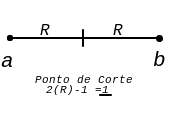
\includegraphics[scale=1]{figs/faixaA-B_PontoCorte.png}
        \caption{Ponto de Corte (R-1)} \label{fig:pontocorte}
\end{figure}

Para haver o ponto de corte antes tem que ser realizado a ordenação dos dados. A largura de cada faixa ${r_1,...,r_R}$ na equação \ref{eq:largurafaixa} é representada por ${w}$, que é calculada pela diferença entre os limites superior e inferior do intervalo, dividido pela quantidade ${R}$ de valores a serem gerados.

\begin{equation}
 w = \frac{b-a}{R}
 \label{eq:largurafaixa}
\end{equation}

A variável ${w}$ determina os pontos de corte ${(c_1,...,c_{R-1})}$ que irão delimitar o tamanho das faixas de valores. O primeiro ponto de corte, ${c_1}$, é obtido através da soma do limite inferior ${a}$ com a tamanho de ${w}$. E os pontos de corte seguintes são calculados pela soma do ponto de corte anterior com ${w}$.


O valor de cada faixa será representado por ${i}$, onde ${i}$ é o índice indicando a faixa. De acordo com a figura \ref{fig:faixasEWD} para dividir o intervalo ${[a,b]}$ em ${R}$ faixas será necessário de ${R-1}$ pontos de corte.

\begin{equation}
c_i=\left\{\begin{matrix}
a+w, & se\, i=1 & \\ 
c_{i-1}+w,  & caso\, contrário & 
\end{matrix}\right.
 \label{eq:regratamfaixa}
\end{equation}

O valor da faixa do intervalo ${[a,c_1]}$ será o valor discreto igual ao índice de sua faixa ${r_1}$. Então, um valor na faixa ${r_1}$ terá o valor reprensentado por ${1(um)}$, pois  ${i=1}$ é o limite inferior mais largura da faixa, equação \ref{eq:regratamfaixa}. E seguindo o mesmo raciocínio o valor da faixa ${r_2=]c_1,c_2]}$ é representado por ${2(dois)}$, e consequentemente o valor que se encontra em uma faixa qualquer ${r_i}$ será reprensentado por ${i}$.

%\afterpage{
\begin{figure}[h] 
        \centering
        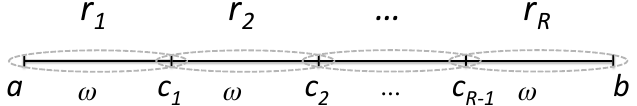
\includegraphics[scale=0.6]{figs/discretizacaoEWD.png}
        \caption[Discretização EWD]{Discretização EWD baseada em \cite{LOPES2014}}%\footnotemark } 
        \label{fig:faixasEWD}
\end{figure}
%\footnotetext{Figura extraída de \cite{Lopes}}
% }



\subsection{Discretização por Frequência Iguais - EFD}\label{cap:refTeor:subsec:efd}

Esse outro método de discretização já possui uma abordagem diferente a do EWD, pois a idéia é manter a quantidade de elementos distintos, entre os pontos de corte, com o mesmo número. Dado um intervalo ${[a,b]}$ o número de faixas ${R}$ e a quantidade de valores distintos ${\xi}$ , onde ${\xi \geqslant R}$ o método EFD irá segmentar em  ${R}$ faixas de valores que possuem a mesma quantidade de elementos distintos ${\lambda}$. Então serão realizados ${R-1}$ pontos de corte gerando ${R}$ faixas de valores, ${(r_1,...,r_R)}$, com a mesma quantidade de elementos distintos ${\lambda}$. Para encontrar ${\lambda}$ calcula-se o valor inteiro da divisão entre a quantidade de elementos distintos ${\xi}$ pela quantidade de faixas de valores ${R}$, obtendo o número de elementos da faixa \ref{eq:qtdelemfaixaEFD}.

\begin{equation}
\lambda = \frac{\xi}{R}
 \label{eq:qtdelemfaixaEFD}
\end{equation}

Uma observação nesse método é a ocorrência em amostras que possuem uma má distribuição de valores de um dado atributo. Como um número significativo de repetições, causando um desiquilíbrio nas distribuições dos elementos.

Uma vez no intervalo ${[a,b]}$ de elemetos ordenado e calculado ${\lambda}$ contendo ${R}$ elementos ${v_{[R]}}$  pode-se determinar os pontos de corte ${(c_1,...,c_{R-1})}$ que são os delimitadores das faixas. Cada ponto de corte ${c_i}$ pode ser calculado por ${v_{i\lambda}-ésimo}$ elemento, \ref{eq:pontocorteEFD}.

\begin{equation}
c_i = v_{[i\lambda]}
 \label{eq:pontocorteEFD}
\end{equation}

Igual o que aconteceu no método EWD, o valor que estiver no intervalo ${[a,c_1]}$ terá seu valor associado a um valor discreto igual ao índice ${i}$ de sua faixa ${r_i}$ conforme figura \ref{fig:faixasEFD}. Então, caso o valor esteja na faixa ${r_2}$ ele passará a ter o valor de seu índice ${i}$ igual a ${2(dois)}$. De maneira consecutiva os valores que estiverem na faixa ${r_3=]c_2,c_3]}$ terão valor ${3(três)}$. Uma outra observação desse método é que diferente do EWD, os intervalos podem assumir faixas com tamanhos diferentes.

%\afterpage{
\begin{figure}[h]
        \centering
        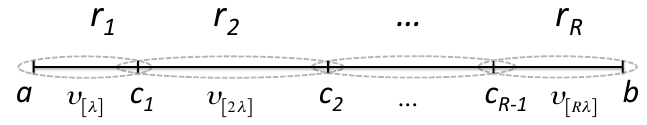
\includegraphics[scale=0.6]{figs/discretizacaoEFD.png}
        \caption[Discretização EFD]{Discretização EFD\footnotemark} 
        \label{fig:faixasEFD}
\end{figure} 
\footnotetext{Figura extraída de \cite{LOPES2014}}
%}


\section{Trabalhos Correlatos}\label{cap:refTeor:sec:trabcorrel}

Esta seção propõe relacionar outros trabalhos servindo de complemento teórico para entender a variedade de aplicações referente ao assunto de rotulação de dados.

O trabalho escrito por \citeonline{LOPES2014} fez um estudo abordando o tema de rotulação de dados, tema este, proposto também por esta pesquisa, mas com abrangência e execução diferentes do modelo da figura \ref{fig:modeloLOPES} . No trabalho de \citeonline{LOPES2014} foi utilizado como entrada um conjunto de dados onde foi feito o agrupamento automático, com algoritmos não-supervisionados formando  clusters. Logo após é utilizado um algoritmo supervisionado (Redes Neurais) nos grupos de dados, e apresentado como saída um rótulo específico que melhor define o grupo formado. Esses rótulos são formados pela faixa de valor, que mais se repetem, em conjunto com os atributos mais relevantes.

Pode-se verificar na figura \ref{fig:modeloLOPES} que na parte onde é aplicado o algoritmo  de redes neurais (processo III) é o local exato que esta pesquisa utiliza para testar outros algoritmos supervisionados, servindo para comprovar a hipótese desta proposta de mestrado e validação do modelo.

\begin{figure}[h]
        \centering
        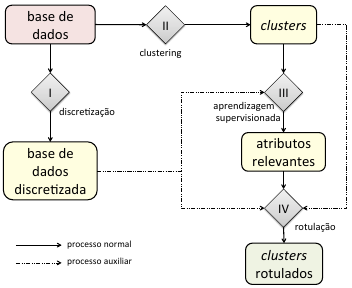
\includegraphics[scale=0.8]{figs/modeloLopes.png}
        \caption{Modelo de \citeonline{LOPES2014}} 
        \label{fig:modeloLOPES}
\end{figure}


Em \citeonline{Metodo2015} o problema em questão é fazer classificação e rotulação em uma base que possuem poucos elementos classificados utilizando método semi-supervisionado. O método inicia com uma base dividida em elementos classificados(L) e não classificados(U). Após cada iteração o grupo L vai crescendo e automaticamente diminuindo o grupo U até que não tenha mais nenhum elemento em U, figura  \ref{fig:modeloVicente}. Após isso é realizado uma etapa de agrupamento, sem levar em consideração os dados classificados anteriormente. Terminada essa etapa é feito uma validação para saber quais os rótulos foram considerados corretos.
\begin{figure}[!h]
        \centering
        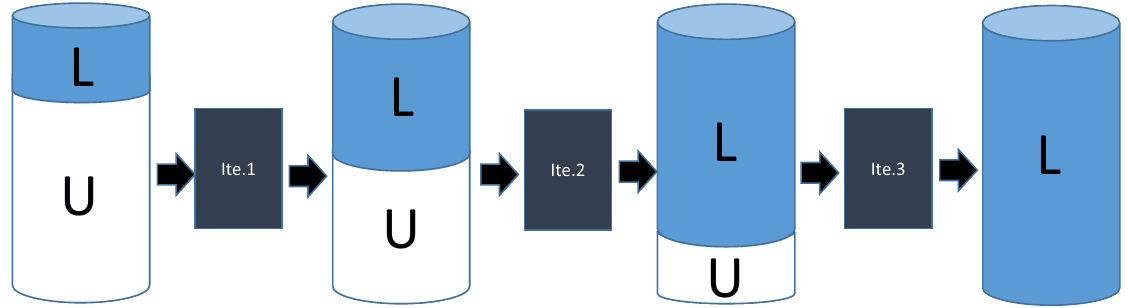
\includegraphics[scale=0.4]{figs/modeloVicente.png}
        \caption{Comportamento da base de dados a cada iteração. Método \cite{Metodo2015}} \label{fig:modeloVicente}
\end{figure}

O método proposto é uma combinação de um classificador com um método de agrupamento, onde a rotulação de um conjunto de dados é feita com conhecimento prévio de um outro conjunto menor rotulado. O classificador treina com a parte de dados rotulada e classifica os dados não-rotulados.


Outra pesquisa sore rotulação está em \cite{Filho2015} onde aborda o mesmo Problema de Rotulação, mas a atuação é diferenciada, pois o modelo procura diferenças existentes em cada grupo através da seleção dos elementos que representam o grupo, e depois é construído a faixa de valores. Os grupos são formados pelo algoritmo Fuzzy C-Means e após isso que é selecionado os atributos. 
% \begin{figure}[!h]
%         \centering
%         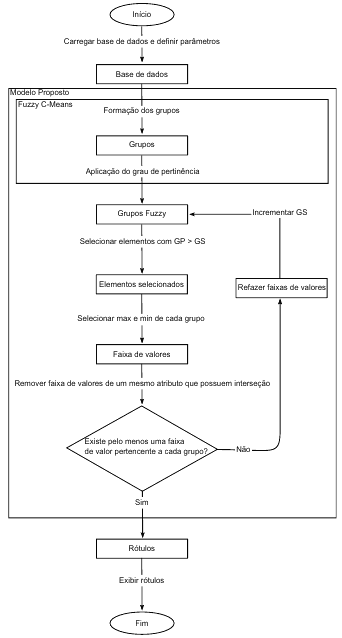
\includegraphics[scale=0.8]{figs/modeloRotFuzzy.png}
%         \caption{Modelo \cite{Filho2015}} \label{fig:modeloFilhoVilmar}
% \end{figure}







\chapter{Metodologia / Materiais e Métodos}\label{cap:ferramentas}
Esse capítulo abordará em uma sessão o problema proposto por esse trabalho, e logo em seguida, será apresentado um modelo de resolução. O objetivo ao final deste capítulo é poder resolucionar o problema, exibindo seus passos, e atribuir a qualquer outro pesquisador todo o conhecimento necessário para replicar este trabalho através das informações produzidas aqui.

\section{Considerações do Problema}

A abordagem do problema referente a essa proposta de mestrado segue uma linha já pequisada por \cite{Lopes}, que seria o \textbf{Problema de Rotulação}. Esse conceito, rotulação de dados,  já é estudado na literatura na área de aprendizagem não-supervisionada, sessão \ref{ssec:aprendNSup}, onde é comum os algoritmos lidarem com os agrupamentos dos dados, onde clusters são criados a partir dos graus similaridade entre os elementos.

Muitas pesquisas realizadas na área de rotulação fazem referencia, de fato, a classificação do dados, e não da rotulação, nos termos desse trabalho. Ao agrupar um conjunto de elementos por um derterminado critério, esta havendo uma classificação desses elementos escolhidos, mas pouco se sabe, qual é a compreensão desses grupos, já classificados. 

Existe uma importância na criação dos clusters, contudo para o espectador é interessante existir um rótulo, desse grupo formado, oferecendo elementos em alguma tomada de decisão em razão de seu significado(rótulo).

Tem-se então o real problema de rotulação, contudo é necessário existir algum elemento definindo o porquê daquele grupo formado. O elemento é um rótulo composto por um, ou vários, atributo(s) de maior relevância no cluster, junto com uma faixa de valores. Essa faixa é um intervalo de valores definido pela discretização \ref{}, onde o intervalo escolhido, seria a faixa que apresenta os valores que se repetem com a maior frequência.

O Problema de Rotulação é formalmente definido como segue abaixo:
\newtheorem{defprob}{Definição}
    \begin{defprob}
    Dado um conjunto de clusters ${C=\{c_1,...,c_k | K \geqslant 1\} }$, de modo que cada cluster contém um conjunto de elementos ${c_i=\{\vec{e}_1,..,\vec{e}_{n^{(c_i)}}|n^{(c_i)} \geqslant 1 \}}$ que podem ser representados por um vetor de atributos definidos em ${\mathbb{R}^m }$ e expresso por ${ \vec{e}^{c_i}=(a_1,..,a_m)  }$ e ainda que  com ${ c_i \cap c_{i'}=\{0\} }$ com ${ 1 \leqslant i, i \leqslant K  }$ e ${ i \neq i' }$.
        \footnotemark 
        \footnotetext{Adaptada de \cite{Lopes}}
        \begin{itemize}[noitemsep]
            \item ${K}$ é o número de clusters;
            \item ${c_i}$ é o i-ésimo cluster qualquer;
            \item ${n^{c_i}}$ é o número de elementos do cluster ${c_i}$;
            \item ${\vec{e}_{n^{(c_i)}}}$ se refere ao j-ésimo elemento pertencente ao cluster ${c_i}$;
            \item ${m}$ é a dimensão do problema;
        \end{itemize}
    \label{teo:problema}
    \end{defprob}

%\afterpage{
%    \begin{quotation}

%        \textit{ Dado um conjunto de clusters ${C=\{c_1,...,c_k | K \geqslant 1\} }$, de modo que cada cluster contém um conjunto de elementos ${c_i=\{\vec{e}_1,..,\vec{e}_{n^{(c_i)}}|n^{(c_i)} \geqslant 1 \}}$ que podem ser representados por um vetor de atributos definidos em ${\mathbb{R}^m }$ e expresso por ${ \vec{e}^{c_i}=(a_1,..,a_m)  }$ e ainda que  com ${ c_i \cap c_{i'}=\{0\} }$ com ${ 1 \leqslant i, i \leqslant K  }$ e ${ i \neq i' }$.
%        }\footnotemark 

%        \footnotetext{Extraída de \cite{Lopes}}
%        \begin{itemize}[noitemsep]
%            \item ${K}$ é o número de clusters;
%            \item ${c_i}$ é o i-ésimo cluster qualquer;
%            \item ${n^{c_i}}$ é o número de elementos do cluster ${c_i}$;
%            \item ${\vec{e}_{n^{(c_i)}}}$ se refere ao j-ésimo elemento pertencente ao cluster ${c_i}$;
%            \item ${m}$ é a dimensão do problema;
%        \end{itemize}
%    \end{quotation}
    %\footnotetext{Extraída de \cite{Lopes}}
%}

\section{O Modelo de Resolução}

Uma vez já conhecido a definição do problema - \textit{Definição ~\ref{teo:problema}} - é possível situar a abrangência abordada aqui nessa pesquisa, pois a intenção do estudo científico desenvolvido aqui é provar a realização de \textbf{rotulação de dados com qualquer algoritmo supervisionado}, utilizando as técnicas abordadas neste texto.

O Modelo aqui proposto consiste em apresentar como saída um conjunto de rótulos, onde cada rótulo específico é dado por um conjunto de pares de valores, atributo e seus respectivo intevalor, gerado a partir da frequência de valores repetidos neste intervalo. Segue \textit{Definição ~\ref{teo:resolucao}} formalizando a saída do modelo:
    \begin{defprob}
    Dado um conjunto de rótulos ${ R=\{ r_{c1},...,r_{ck} \} }$, no qual cada rótulo específico é dados por um conjunto de pares de valores, tem como saída um vetor com atributo e seu respectivo intervalo, ${ r_{ci}=\{ (a_1,[p_1,q_1]),...,(a_{m^{(c_i)}}, ]p_{m^{(c_i)}},q_{m^{(c_i)}}]) \} }$ capaz de melhor expressar o cluster ${c_i}$.
        \footnotemark 
        \footnotetext{Adaptada de \cite{Lopes}}
        \begin{itemize}[noitemsep]
            \item ${k}$ número de rótulos;
            \item ${R}$ representa o conjunto de rótulos na saída do modelo;
            \item ${a}$ é o atributo
            \item ${c_i}$ é o i-ésimo cluster;
            \item ${r_{c_i}}$ é o rótulo referente ao cluster ${c_i}$;
            \item ${]p_{m^{(c_i)}},q_{m^{(c_i)}}]}$ representa o intervalo de valores do atributo ${a_{m^{(c_i)}} }$, onde ${ p_{m^{(c_i)}} }$  é o limite inferior e ${ q_{m^{(c_i)}} }$ é o limite superior;
            \item ${m}$ é a dimensão do problema;
        \end{itemize}
    \label{teo:resolucao}
    \end{defprob}

Como apresentado na sessão \ref{sec:trabcorrel}, o autor foca em rotulação automática de grupos utilizando a estratégia de aprendizagem de máquina supervisionada, e paradigma conexionista, para provar seu trabalho. Mas aqui nessa pesquisa foi aplicado no modelo um acréscimo de ${2 (dois)}$ algoritmos com paradigmas de aprendizado diferentes do que já foi utilizado, compondo uma base para afirmar, que a partir dessas amostras pode-se fazer rotulação com qualquer algoritmo supervisionada.


\begin{figure}[h!]
        \centering
        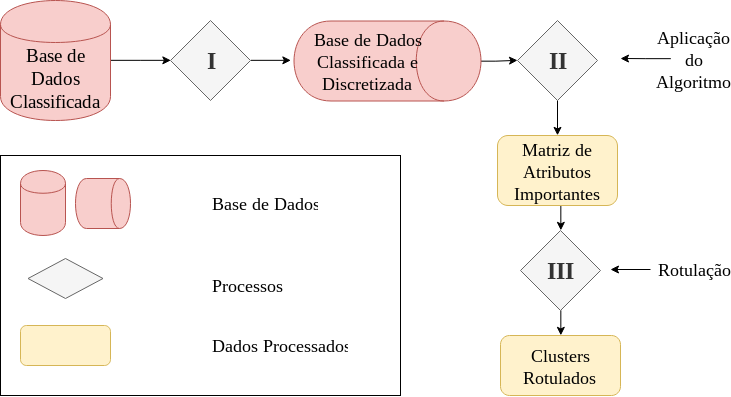
\includegraphics[scale=0.7]{figs/modeloResolucao.png}
        \caption{Modelo de Resolução Proposto} \label{fig:modeloresolucao}
\end{figure}

O modelo, figura \ref{fig:modeloresolucao}, inicialmente mostra a Base de Dados  já classificada, pois o cerne desta pesquisa é conceder ao grupo um significado,a rotulação,  através da técnica de correlação entre atributos, sessão ~\ref{sec:tecnica}. Essa base poderá conter  valores contínuos ou discretos, contudo, conforme modelo será necessário aplicar o método de discretização (I).

Uma vez com a base discretizada ocorre somente a separação dos clusters já classificados de acordo com a própria base de dados\footnote{UCI - Machine Learning Repository. http://archive.ics.uci.edu/ml/ }. Isso é o funcionamento do fluxo (a), que nada mais é do que a separação da base em grupos que já classificados.

No passo (II) é onde serão executados os algoritmos de aprendizagem supervisionado, já visto nas sessões ~\ref{sssec:cart} e ~\ref{sssec:nbayes}. Essa etapa é umas das mais importantes do método. O algoritmo supervisionado é aplicado várias vezes de acordo com o número de atributos do conjunto de dados, expresso no vetor de tamanho ${m}$. Onde o número de vezes será a quantidade de atributos da tabela, formando um conjunto de atributos importantes para cada grupo.

Seguindo para o processo (III) acontecerá a escolha do atributo mais relevante com seu valor mais frequente gerando rótulos para os grupos. Após essa etapa é criado um conjunto de rotulos para cada clusters. O fluxo (b) será utilizado caso houver algoritmo para ser executado.

\section{Técnica de Correlação entre Atributos }\label{sec:tecnica}

Essa técnica \footnote{Extraída  de \cite{Lopes}} possui um grau de processamento diretamente proporcional a quantidade de características expressa na base de dados definido em ${R^m}$. Ela implica em utilizar todos os atributos, menos o definido como classe, para fazer uma correlação entre eles junto ao algoritmo.


Pegando como exemplo uma base com os seguintes atributos: \textbf{atr1,atr2,atr3,classe}. Exclui o atributo classe, obtêm-se os ${3 (três)}$ primeiros atributos, onde cada um deles será utilizado como classe em refência aos outros atributos. 

Em um primeiro processamento de três, o primeiro atributo \textbf{atr1} se torna classe e executado com os outros dois atributos restantes com um algoritmo supervisionado. O resultado da correlação entre os atributos \textbf{atr2, atr3} em relação ao \textbf{atr1}(figura ~\ref{fig:tecnicamodelo} ) é armazanado em uma matriz, e logo depois é realizado com \textbf{atr2} sendo classe e assim sucessivamente até o último atributo.


\begin{figure}[h!]
        \centering
        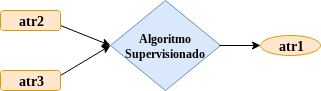
\includegraphics[scale=0.7]{figs/tecnicamodelo.png}
        \caption{Exemplo da técnica aplicada ao atr1 sendo classe } \label{fig:tecnicamodelo}
\end{figure}


\section{Exemplo com Base Modelo}

Para melhor esclarecer as etapas da figura \ref{fig:modeloresolucao}, a tabela ~\ref{tab:bdm} contém uma base de dados que será utilizada para exemplificar todo o processo do modelo de resolução proposto nesta pesquisa. Logo na primeira coluna da tabela, retém um índice da linha da tabela responsável por identificar cada registro. Os outros campos são atributos que definem características do registro identificado pelo índice da primeira coluna.

\begin{table}[!ht]
\centering
\caption{Base de Dados Modelo}
\label{tab:bdm}
\begin{tabular}{|lllll|}
\hline 
  & atr1 & atr2 & atr3 & classe \\ \hline
1 & 2.08 & 92.11 & 22.07 & 2 \\ \hline
2 & 1.26 & 85.03 & 20.45 & 1 \\ \hline
3 & 2.00 & 108.36 & 22.68 & 2 \\ \hline
4 & 1.74 & 43.78 & 18.72 & 3 \\ \hline
5 & 1.82 & 100.20 & 23.09 & 2 \\ \hline
6 & 1.43 & 77.59 & 21.80 & 1 \\ \hline
7 & 1.53 & 44.01 & 20.98 & 3 \\ \hline
8 & 1.14 & 107.77 & 18.99 & 2 \\ \hline
9 & 1.97 & 98.00 & 22.32 & 2 \\ \hline
10 & 1.50 & 39.67 & 21.78 & 3 \\ \hline
11 & 1.74 & 55.86 & 20.31 & 3 \\ \hline
12 & 1.80 & 65.72 & 19.62 & 1 \\ \hline
13 & 1.33 & 82.01 & 19.82 & 1 \\ \hline
14 & 1.66 & 103.93 & 21.10 & 2 \\ \hline
15 & 1.42 & 66.14 & 21.61 & 1 \\ \hline
16 & 1.87 & 88.36 & 22.45 & 2 \\ \hline
17 & 1.11 & 107.82 & 19.32 & 2 \\ \hline
18 & 2.08 & 67.66 & 20.74 & 1 \\ \hline
19 & 1.85 & 82.65 & 20.35 & 1 \\ \hline
20 & 1.04 & 102.62 & 19.46 & 2 \\ \hline
21 & 1.97 & 100.37 & 21.94 & 2 \\ \hline
22 & 1.95 & 45.70 & 22.10 & 3 \\ \hline
23 & 1.77 & 50.04 & 20.16 & 3 \\ \hline
24 & 1.97 & 81.57 & 19.83 & 1 \\ \hline
25 & 1.52 & 93.13 & 20.61 & 2 \\ \hline
  \end{tabular}
  \begin{tabular}{ |lllll| }
   
\hline
  & atr1 & atr2 & atr3 & classe \\ \hline
26 & 1.42 & 53.51 & 19.64 & 3 \\ \hline
27 & 1.12 & 62.71 & 19.07 & 1 \\ \hline
28 & 2.09 & 60.58 & 20.20 & 1 \\ \hline
29 & 1.95 & 69.23 & 19.68 & 1 \\ \hline
30 & 1.03 & 47.81 & 19.47 & 3 \\ \hline
31 & 1.75 & 90.92 & 21.39 & 2 \\ \hline
32 & 1.72 & 42.35 & 22.89 & 3 \\ \hline
33 & 1.47 & 101.77 & 19.20 & 2 \\ \hline
34 & 1.53 & 41.16 & 22.67 & 3 \\ \hline
35 & 1.44 & 93.61 & 21.03 & 2 \\ \hline
36 & 1.51 & 98.65 & 19.24 & 2 \\ \hline
37 & 1.06 & 68.82 & 21.68 & 1 \\ \hline
38 & 1.48 & 80.40 & 21.43 & 1 \\ \hline
39 & 1.14 & 61.59 & 19.90 & 1 \\ \hline
40 & 1.08 & 91.93 & 20.81 & 2 \\ \hline
41 & 1.62 & 79.21 & 18.43 & 1 \\ \hline
42 & 1.68 & 80.87 & 18.42 & 1 \\ \hline
43 & 1.81 & 98.24 & 22.13 & 2 \\ \hline
44 & 1.30 & 69.27 & 18.83 & 1 \\ \hline
45 & 1.80 & 101.21 & 21.61 & 2 \\ \hline
46 & 1.79 & 72.02 & 22.02 & 1 \\ \hline
47 & 1.56 & 81.71 & 22.10 & 1 \\ \hline
48 & 1.98 & 77.16 & 21.71 & 1 \\ \hline
49 & 1.86 & 89.12 & 22.84 & 2 \\ \hline
50 & 1.55 & 76.01 & 19.74 & 1 \\ \hline
\end{tabular}
\end{table}

Seguindo a definição ~\ref{teo:problema} um elemento é expresso por um vetor  de dimensão ${m}$, com tamanho igual ao número de atributos. Um exemplo do elemento 2 da tabela ~\ref{tab:bdm}, pode ser representado por ${\vec{e}_{2}=(1.26,85.03, 20.45)}$.

\subsection{Processo (I) - Discretização}

Segundo \cite{Catlett2006, Hwang2002} o processo de discretização na etapa de treinamento pode aumentar a acurácia do algoritmo de aprendizado supervisionado. Dessa maneira a etapa de discretização ganha um papel importante no modelo, e também no processo de Rotulação (III), pois é utilizada uma inferência na faixa discretizada para encontrar o intervalo na faixa.

Para esse exemplo será utilizada a técnica de discretização por frequências iguais - EFD - e divisão de números de faixas, igual a R=3. Na figura\footnote{Figura adaptada de \cite{Lopes}} \ref{fig:EFD_R_3} poderá ser vizualizado como é feita a discretização.
 \begin{figure}[h!]
    \centering
    \subfloat[Discretização em atr1]{
        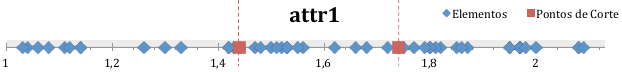
\includegraphics[scale=0.8]{figs/discretizacaoEFD_R_3_atr1.png}
        \label{fig:EFD_R_3:efd:atr1} }
    
    \subfloat[Discretização em atr2]{
        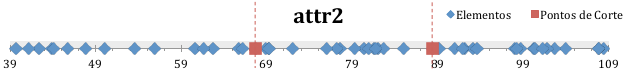
\includegraphics[scale=0.8]{figs/discretizacaoEFD_R_3_atr2.png}
        \label{fig:EFD_R_3:efd:atr2} }
    
    \subfloat[Discretização em atr3]{
        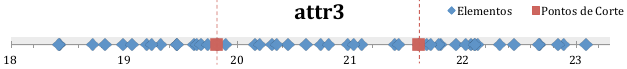
\includegraphics[scale=0.8]{figs/discretizacaoEFD_R_3_atr3.png}
        \label{fig:EFD_R_3:efd:atr2} } 
    
    \caption{Discretização de atributos utilizando EFD com R = 3} \label{fig:EFD_R_3}
        
        %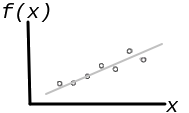
\includegraphics[scale=0.4]{figs/grafB.png}
        %\caption{Polinômio Superajustado} \label{grafB}
\end{figure}
Através da figura \ref{fig:EFD_R_3} fica claro o conteúdo da faixa 1, contendo os valores iniciais até o primeiro ponto de corte, na faixa 2, são os valores após o primeiro ponto de corte até o segundo ponto de corte. E na faixa 3 contém todos  valores a partir do segundo ponto de corte.


\begin{table}[!ht]
\centering
\caption{Base de Dados Modelo Discretizada}
\label{tab:bdmd}
\begin{tabular}{|lllll|}
\hline 
  & atr1 & atr2 & atr3 & classe \\ \hline
1	&	3	&	3	&	3	&	2	\\	\hline
2	&	1	&	2	&	2	&	1	\\	\hline
3	&	3	&	3	&	3	&	2	\\	\hline
4	&	2	&	1	&	1	&	3	\\	\hline
5	&	3	&	3	&	3	&	2	\\	\hline
6	&	1	&	2	&	3	&	1	\\	\hline
7	&	2	&	1	&	2	&	3	\\	\hline
8	&	1	&	3	&	1	&	2	\\	\hline
9	&	3	&	3	&	3	&	2	\\	\hline
10	&	2	&	1	&	3	&	3	\\	\hline
11	&	2	&	1	&	2	&	3	\\	\hline
12	&	3	&	1	&	1	&	1	\\	\hline
13	&	1	&	2	&	1	&	1	\\	\hline
14	&	2	&	3	&	2	&	2	\\	\hline
15	&	1	&	1	&	2	&	1	\\	\hline
16	&	3	&	2	&	3	&	2	\\	\hline
17	&	1	&	3	&	1	&	2	\\	\hline
18	&	3	&	1	&	2	&	1	\\	\hline
19	&	3	&	2	&	2	&	1	\\	\hline
20	&	1	&	3	&	1	&	2	\\	\hline
21	&	3	&	3	&	3	&	2	\\	\hline
22	&	3	&	1	&	3	&	3	\\	\hline
23	&	3	&	1	&	2	&	3	\\	\hline
24	&	3	&	2	&	2	&	1	\\	\hline
25	&	2	&	3	&	2	&	2	\\	\hline
  \end{tabular}
  \begin{tabular}{ |lllll| }
   
\hline
  & atr1 & atr2 & atr3 & classe \\ \hline
26	&	1	&	1	&	1	&	3	\\	\hline
27	&	1	&	1	&	1	&	1	\\	\hline
28	&	3	&	1	&	2	&	1	\\	\hline
29	&	3	&	2	&	1	&	1	\\	\hline
30	&	1	&	1	&	1	&	3	\\	\hline
31	&	3	&	3	&	2	&	2	\\	\hline
32	&	2	&	1	&	3	&	3	\\	\hline
33	&	2	&	3	&	1	&	2	\\	\hline
34	&	2	&	1	&	3	&	3	\\	\hline
35	&	1	&	3	&	2	&	2	\\	\hline
36	&	2	&	3	&	1	&	2	\\	\hline
37	&	1	&	2	&	3	&	1	\\	\hline
38	&	2	&	2	&	2	&	1	\\	\hline
39	&	1	&	1	&	2	&	1	\\	\hline
40	&	1	&	3	&	2	&	2	\\	\hline
41	&	2	&	2	&	1	&	1	\\	\hline
42	&	2	&	2	&	1	&	1	\\	\hline
43	&	3	&	3	&	3	&	2	\\	\hline
44	&	1	&	2	&	1	&	1	\\	\hline
45	&	3	&	3	&	2	&	2	\\	\hline
46	&	3	&	2	&	3	&	1	\\	\hline
47	&	2	&	2	&	3	&	1	\\	\hline
48	&	3	&	2	&	3	&	1	\\	\hline
49	&	3	&	3	&	3	&	2	\\	\hline
50	&	2	&	2	&	1	&	1	\\	\hline

\end{tabular}
\end{table}

A tabela \ref{tab:bdmd} é o resultado após a discretização de todos os atributos. Contudo sabe-se que ao se lidar com valores discretos onde cada intervalo representa uma faixa de valores poderá o algoritmo está perdendo um pouco de informação, mas por outro lado essa decisão tornará o aprendizado mais fácil de interpretar e com respostas mais rápidas.

\subsection{Processo (II) - Algoritmos Supervisionados}

Ao chegar nessa etapa, Processo (II) da figura \ref{fig:modeloresolucao}, já se tem uma base discretizada e clusters formados, tabela \ref{tab:bdmd}. Agora é feita a execução do algorimo de aprendizado supervisionado e identificado os atributos de maior importância de cada cluster.

Uma vez com o conhecimento do cluster, serão percorridos todos os atributos, onde a cada iteração um atributo será a classe da vez. Nesse exemplo primeiramente o atributo \textbf{atr1} será classe, e os demais irão participar como entrada junto ao algoritmo, e verificar seu grau de importância entre eles. Depois o atributo \textbf{atr2} irá ser classe, e depois o \textbf{atr3}, fechando o ciclo de todos os atributos do cluster. Como visualizado na figura \ref{fig:tecnicamodelocomp} 
\begin{figure}[h!]
        \centering
        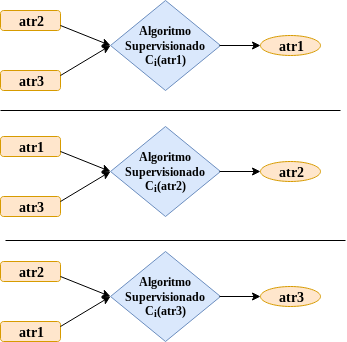
\includegraphics[scale=0.7]{figs/tecnicamodeloComp.png}
        \caption{Exemplo da técnica aplicada aos ${3 (três)}$ atributos, cada um sendo classe em determinada iteração } \label{fig:tecnicamodelocomp}
\end{figure}

Essa correlação entre os atributos junto com a aplicação dos algoritmos geram uma matriz de atributos importantes. O quão relevante o atributo será em relação ao cluster ${c_i(atr)}$, será dado em uma porcentagem de acerto quando aplicado como saída na execução de um algorimo supervisionado. Quanto maior sua porcentagem, mais correlacionado é o atributo em relação ao demais(figura \ref{fig:rotulacao}), logo ele é considerado um atributo bem relevante. Sendo assim esse atributo poderá resumir as características do problema, podendo ser considerado um atributo importante e escolhido como rótulo.

 \begin{figure}[h!]
    \centering
    \subfloat[Execução do Naive Bayes]{
        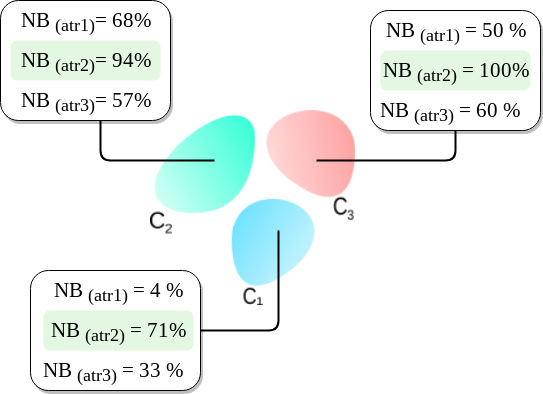
\includegraphics[scale=0.3]{figs/rotulacaoNB.png}
        \label{fig:rotulacao:rotNB} }
    \quad
    \subfloat[Execução do algorimo de Árvore de Decisão]{
        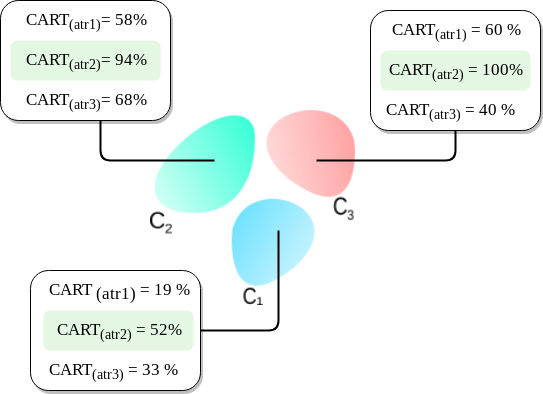
\includegraphics[scale=0.3]{figs/rotulacaoDecisionTree.png}
        \label{fig:rotulacao:rotDT} } 
    
    \caption{Resultado dos Algoritmos} \label{fig:rotulacao}
        %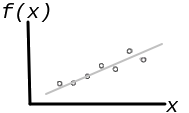
\includegraphics[scale=0.4]{figs/grafB.png}
        %\caption{Polinômio Superajustado} \label{grafB}
\end{figure}

Na figura \ref{fig:rotulacao:rotNB} mostra o resultado da execução do Naive Bayes em cima da Base Modelo e exibe os resultados em porcentagem de acerto de cada atributo em relação aos demais. O mesmo acontece com a figura \ref{fig:rotulacao:rotDT} onde é aplicado um algorimo de Árvore de Decisão, exibindo o resultado de todas as taxas de acerto, em porcentagem, dos atributos de seus respectivos clusters.

Uma forma de eliminar uma possível ambiguidade entre os clusters foi adicionar uma variável  ${V}$. Com essa variável a seleção dos atributos rótulos de um clusters, seram todos os atributos que tiverem até uma diferença ${V}$ em relação ao atributo de maior taxa de acerto, expresso em porcentagem. Portanto se o atributo de maior taxa de acerto possuir ${90\%}$, e o ${V=10\%}$  então todos outros atributos que tiverem valores a partir de ${80\%}$ seram selecionados como rótulo do cluster.  

O valor da variável ${V}$ é subjetivo e irá ser arbitrado de acordo com os resultados em cada aplicação do algoritmo em cima de um conjunto de dados. Nese exemplo os atributos importantes com ${V=12}$ utilizando a figura \ref{fig:rotulacao:rotNB} por cluster, teriam os rótulos ${r_{c_i}}$ : ${r_{c_1}=\{atr2\}}$, ${r_{c_2}=\{atr2\}}$, ${r_{c_3}=\{atr2\}}$.

\subsection{Processo (III) - Rotulação}

Nesse processo de rotulação serão calculados os intervalos dos atributos que estão na figura \ref{fig:modeloresolucao} como Atributos Importantes, selecionados na etapa anterior. Para compor o rótulo ${r_{c_i}}$ do cluster ${c_i}$ é calculado a faixa do atributo  que tiver maior frequência. 
É possível verificar neste exemplo, da Base Modelo, o resultado da figura \ref{fig:rotulacao:rotNB}, onde o rótulo ${r_{c_1}}$ é o  \textbf{atr2=]67.66, 88.36]}, porque o valor da faixa de maior frequência do cluster ${c_1}$ em relação ao atributo \textbf{atr2} é a faixa 2(figura \ref{fig:EFD_R_3:efd:atr2}), que é representa o limite inferior ${]67.66}$s e o limite superior, ${88.36]}$.

Uma vez terminado o processo (III) de rotulação, o fluxo ${b}$ do modelo da figura \ref{fig:modeloresolucao}, só é seguido caso seja necessário para executar outro algoritmo.

Contudo pode-se definir os rótulos nesta etapa da seguinte maneira:


\begin{itemize}[noitemsep]
            \item Algoritmo Naive Bayes  \ref{fig:rotulacao:rotNB} aplicado na BD Modelo
            \subitem ${r_{c_1}=(atr2,]67.66, 88.36])}$;
            \subitem ${r_{c_2}=(atr2,]88.36, 108.36])}$ ;
            \subitem ${r_{c_3}=(atr2,[39.67, 67.66])}$;
            
            \item Algoritmo de Árvore de Decisão  \ref{fig:rotulacao:rotDT} aplicado na BD Modelo
            \subitem ${r_{c_1}=(atr2,]67.66, 88.36])}$;
            \subitem ${r_{c_2}=(atr2,]88.36, 108.36])}$ ;
            \subitem ${r_{c_3}=(atr2,[39.67, 67.66])}$;
\end{itemize}

Logo abaixo o algoritmo \ref{alg:rotulacao} exibe a rotina em forma de pseudocódigo para melhor entendimento.

\IncMargin{1em}
\begin{algorithm}[h]

\nl $Carrega\_valores\_auxiliares(V,R,TipoDiscretização)$\;
\nl $Carrega\_BD$\; 
\nl $Discretiza\_BD$\; 
\nl $Separa\_em\_clusters\_de\_acordo\_com\_classificação\_BD$\; 
\nl \While{existir clusters}{
 \nl \While{existir atributos}{ 
      \nl $prepara\_vetor\_atributos/classe$\; 
      \nl $Aplica\_algoritmo\_supervisionado$\;
      \nl $Calcula\_matriz\_de\_porcentagem\_de\_acertos$\; 
      } 
    \nl $Carrega\_atributos\_importantes\_considerando\_V$\;
    \nl $Associa\_valores\_aos\_intervalos$\; 
 }
 \nl $Exibe\_rótulos\_todos\_clusters$\; 
 \caption{Rotina de Rotulação}\label{alg:rotulacao}
 
\end{algorithm}
\DecMargin{1em}
        

% PARTE
%\part{Proposta}
%\chapter{Sistema Proposto}\label{cap:proposta}

Esse trabalho propõe um sistema de... 


\section{Primeira Parte do Sistema Proposto}

\lipsum[67]

\section{Considerações Finais}

\lipsum[68]

% PARTE
%\part{Parte Final}
 \chapter{Resultados e Discussões}\label{cap:resultados}


Este estudo conta com a realização de testes nas bases de dados da UCI Machine Learning\footnote{http://archive.ics.uci.edu/ml/} - um repositório de dados a serviço da comunidade de aprendizado de máquina criado por estudantes de pós-graduação na UC Irvine em 1987 e que é utilizado por educadores e pesquisadores como fonte primária de aplicações de aprendizado de máquina. 
 


As bases de dados escolhidas para este trabalho foram: Seeds, Iris, Glass, Wine. Essas bases são bastante utilizadas em vários trabalhos\footnote{https://archive.ics.uci.edu/ml/datasets/glass+identificpation, https://archive.ics.uci.edu/ml/datasets/iris, https://archive.ics.uci.edu/ml/datasets/wine, https://archive.ics.uci.edu/ml/datasets/seeds} e por meio delas há possibilidade de análise de seus comportamentos mediante  resultados dos mesmos. As bases selecionadas são todas classificadas, tendo em vista que este estudo são com  \textit{clusters} já contituídos e não na formação deles. Outro motivo desta seleção, é elaborar testes com bases de organização simple, \textit{i.e.}, não sejam necessárias empregar técnicas de manipulação de dados  \cite{Casari2018} na fase de preparação (inicial) para efetuar os testes.

Foram apresentadas em todos os resultados, tabelas com algumas informações da rotulação realizada pelos algoritmos nas determinadas bases,  com o seguinte formato: a primeira coluna (\textbf{Cluster}) é um número que representa cada \textit{cluster} de forma sequencial; a segunda coluna (\textbf{Rótulos}) é representada pelo par \textbf{Atributo} e \textbf{Faixa}, o qual define o rótulo do \textit{cluster} respectivo, podendo haver ou não mais atributos para compor o rótulo; a coluna \textbf{Elementos Fora da Faixa}, exibe o erro em quantidade de elementos que não estão naquela faixa definida naquele rótulo e, por último, a \textbf{Acurácia Parcial}, que exibe, em porcentagem, o valor de acertos dos elementos que são representados pelo atributo e faixa da respectiva linha. 

Quaisquer resultados da aplicação dos algoritmos supervisionados nos \textit{clusters} a fim de encontrar os rótulos podem ser confrontados com as informações dos \textit{clusters} inicialmente retirados da \textit{UCI Machine Learning} e, assim, calculada a porcentagem de acertos, mediante análise dos registros que estão representados pelo rótulo.


A divisão deste capítulo iniciará por uma explanação da implementação do trabalho, explicando as ferramentas utilizadas no desenvolvimento, bem como os algoritmos e  as configurações de algumas variáveis, e cada seção referir-se-á a uma base de dados utilizada, sendo esta dividida em subseções para os seguintes algoritmos: Naive Bayes, CART e KNN. 

\section{Implementação}\label{cap:resultados:sec:implement}


Ao longo da pesquisa foram realizados vários testes, porém, houve alterações de algumas variáveis e métodos de discretização, sempre com o objetivo de obter os melhores resultados. As variáveis e métodos alterados são: variância (${V}$ ), número de faixas (${R}$) e tipo de discretização ${TipoDiscretização}$ (EWD,EFD). 


Fazendo um breve resumo sobre as configurações das variáveis, a variação ${V}$ existe para evitar a ambiguidade dos rótulos, ou seja, para quando os rótulos apresentarem os mesmos resultados: atributo e faixa de valor. O número de faixas (${R}$) é definido de forma que os atributos tenham seus valores mapeados de acordo com a faixa de valor correspondente e, uma vez definido o número de faixas, será escolhido qual método de discretização será aplicado (EWD,EFD), decidindo-se com qual faixa cada valor irá ficar.

Algumas outras características da implementação estão dispotas no Apêndice \ref{apendice:2}

%Fazendo um breve resumo sobre as configurações das variáveis, a variação ${V}$ existe para evitar a ambiguidade dos rótulos, ou seja, quando os rótulos apresentarem os mesmos resultados: atributo e faixa de valor. O número de faixas (${R}$), é o número de faixas definido de forma que os atributos tenham seus valores mapeados de acordo com o valor da variável, e dependendo de como os dados do atributo são dispostos, existirá uma melhor divisão no número de faixas \footnote{Apêndice \ref{apendice:1}}, contudo, os resultados foram realizados com ${R=3}$ em concordância ao trabalho de \citeonline{Lopes2016} que também utilizou esse configuração, e assim podendo haver uma comparação entre resultados. Uma vez definido o número de faixas será escolhido qual método de discretização será aplicado (EWD,EFD), decidindo qual faixa cada valor irá ficar.  



%Além de evitar a ambiguidade dos rótulos a variável ${V}$ pode ser utilizada também para selecionar mais de um atributo para ser o rótulo do cluster. 


%A utilização da variação ${V}$ para escolha de rótulos acontece após uma análise da tabela de correlação dos atributos (seção \ref{cap:ferramentas:sec:tecnica}), a exemplo da tabela \ref{tab:matrelevancia:seeds:nb}. E existindo valores muito próximos em relação a outros (cabe a uma análise se necessário), poderá utilizar esses atributos também como rótulos para melhor definir o cluster. A variável ${V}$ pode ser configurada com um valor que possa abranger esses atributos que possuam valores de porcentagens próximos ao do atributo de maior valor na tabela (mais relevante). O valor de ${V}$ é subjetivo e sua adição é condicionada a análise da aplicação do algoritmo na bases de dados.

%É importante ressaltar a criação da tabela de correlação de atributos (Matriz de Atributos Importantes). Essa tabela é implementada conforme a técnica de correlação entre atributos com algoritmos supervisionados, seção \ref{cap:ferramentas:ssec:algsuper}, onde cada célula da tabela é preenchida através da execução de um algoritmo supervisionado. Estas execuções são realizadas em todos os atributos da cada cluster existente na base de dados.

%Após a tabela preenchida, o atributo rótulo será selecionado a partir do maior valor em relação aos outros atributos do grupo, que é representado pela linha da tabela (matriz de atributos). Também poderá ser selecionado como rótulo os atributos que possuam o valor entre a diferença de ${V}$ com o atributo de maior valor (mais relevante). Por exemplo, se o valor de ${V=5\%}$ e o atributo de maior valor é \textbf{95\%}, então todos os atributos que possuírem o valor a partir de \textbf{90\%} serão considerados rótulos também.

%a cada iteração do algoritmo é preenchida uma célula da tabela com o valor de correlação do primeiro atributo até o último atributo de um cluster, e depois iniciado o mesmo procedimento a outro cluster até não haver mais clusters. Após a tabela estar montada o atributo rótulo será selecionado a partir do maior valor em relação aos outros atributos do grupo, e caso seja necessário também é selecionado como rótulo os atributos que possuam o valor entre a diferença de ${V}$ com o atributo de maior valor (mais relevante). 


%A cada base de dados descritas nas seções seguintes, são configuradas algumas variáveis, método de discretização e implementado dois algoritmos de aprendizado supervisionado com paradigmas diferentes para fazer rotulação. Cada algoritmo terá como resultado o rótulo por cluster de dados.


\section{Base de Dados 1 - Seeds - Identificação de Tipos de Semente}
Essa base é composta por sete  atributos definindo suas características e mais um: a  classe, que é responsável por identificar os tipos de sementes \cite{Charytanowicz2010}. Esses elementos foram construídos a partir de sete parâmetros geométricos medidos dos grãos de trigo: \textit{area} - A, \textit{perimeter} - P, \textit{compactness} - C, \textit{length of kernel} - Lkernel, \textit{width of kernel} - Wkernel, \textit{asymmetry coefficient} - asymetry, \textit{length of kernel groove} - lkgroove.


Os valores dos atributos são todos contínuos e não existem valores em branco, possuindo um total de 210 registros classificados em três categorias bem distribuídas entre as classes, definindo-se estas como base de dados balanceada, por causa dessa distribuição dos registros:

\begin{itemize}[noitemsep]
 \item 70 elementos do tipo \textit{Kama};
 \item 70 elementos do tipo \textit{Rosa};
 \item 70 elementos do tipo \textit{Canadian}.
\end{itemize}


Para classificar as sementes como \textit{Kama}, \textit{Rosa} e \textit{Canadian}, foi utilizada uma técnica de raio X que é relativamente mais barata que outras técnicas de imagem, como microscopia ou tecnologia a laser. O material foi colhido de campos experimentais explorados no Instituto de Agrofísica da Academia Polonesa de Ciências em Lublin. 

As tabelas com os resultados dos rótulos apresentadas a seguir (tabelas \ref{tab:rot:seeds:nb},\ref{tab:rot:seeds:cart}, \ref{tab:rot:seeds:knn}) exibem os resultados de rotulação dos algoritmos Naive Bayes, CART e KNN, respectivamente, e no caso dos \textit{clusters}, cada linha determina um grupo: (1) \textit{Kama}, (2) \textit{Rosa} e (3) \textit{Canadian}. Como já mencionado neste capítulo, na seção \ref{cap:resultados:sec:implement}, antes de executar o algoritmo, algumas configurações são necessárias para executar o algoritmo, como a do método de discretização do tipo EFD ou EWD, e também a divisão dos valores dos atributos em faixas e variação ${v}$.

\subsection{Rotulação através do algoritmo Naive Bayes} \label{cap:resultados:ssec:seed:nb}



Na tabela \ref{tab:rot:seeds:nb} pode-se verificar o resultado da aplicação do algoritmo e através dela percebe-se que o pior rótulo foi no \textit{cluster} 1, com acurácia de 70\%, e com isso deixa de representar nove registros no total de setenta amostras, mas nos outros dois \textit{clusters} a acurácia sobe para 88\%, com um erro de nove registros, porém, os rótulos nestes \textit{clusters} são diferentes, coincidindo somente os valores das colunas \textbf{Elementos Fora da Faixa} e \textbf{Acurácia Parcial}. 

\begin{table}[!ht]
\centering
\caption{Resultado da rotulação com o algoritmo Naive Bayes}
\label{tab:rot:seeds:nb}
\scalebox{0.8}{
\begin{tabular}{llccc}
\hline \hline
\multicolumn{1}{c}{\cellcolor[HTML]{FFFFFF}} & \multicolumn{2}{c}{Rótulos}                & \multicolumn{1}{r}{}               &  \\ \cline{2-3}
Cluster                                      & Atributos      & \multicolumn{1}{c}{Faixa} & Elementos Fora da Faixa & Acurácia Parcial(\%) \\ \hline \hline
1                                            & Lkernel           & ] 5.357 $\sim$  5.826 ]   &  21 & 70\% \\  \hline
2                                            & lkgroove           & ] 5.791 $\sim$  6.55 ]   &  9 & 87.15\%\\ \hline
%\multirow{-2}{*}{2}                          & lkernel        & ] 5.826 $\sim$  6.675 ]   & 92\%                               & 6\\  \hline
3                                            & wkernel      & [ 2.63 $\sim$  3.049 ]   &  9 & 87.15\% \\ \hline \hline
\end{tabular}
}
\end{table}



%Na última coluna, \textbf{Acurácia Parcial}, apresenta em porcentagem o grau de acerto, por \textit{cluster}, dos registros que são representados pelo rótulo. Essa acurácia é possível, visto que, na descrição do \textit{dataset} da  \textit{UCI Machine Learning}\footnote{repositório de dados de onde está a base de dados. https://archive.ics.uci.edu/ml/datasets/seed} já é definido que cada grupo possui 70 (setenta) registros, e quais elementos fazem parte de cada \textit{cluster}. Já em uma análise desta tabela, os valores da coluna Relevância tiveram valore baixos, contudo, uma referência da qualidade do rótulos é diante dos elementos que ficam fora da faixa indicando o grau de representatividade do rótulo.


A última coluna, \textbf{Acurácia Parcial}, apresenta em porcentagem o grau de acerto, por \textit{cluster}, dos registros que são representados pelo rótulo. O grau de confiabilidade passa a ser o número de erros dele, pois quanto menores são os erros mais representabilidade possui o rótulo, dessa forma o menor valor de acurácia ficou em 70\% (setenta por cento) no \textit{cluster} 1, indicando que, dentre as setenta amostras, 21 (vinte e um) não são representadas pelo rótulo, e nos outros \textit{clusters} acima de 87\% (oitenta e sete por cento). 

Segue abaixo o resultado do algoritmo Naive Bayes na base de dados \textbf{Seeds} com seus rótulos: 
\begin{itemize}[noitemsep]
 \item ${r_{c_1}=\{ (Lkernel, ] 5.357 \sim  5.826 ]) \} }$  
 \item ${r_{c_2}=\{ (lkgroove, ] 5.791 \sim  6.55]) \} }$
 \item ${r_{c_3}=\{ (wkernel, [2.63 \sim  3.049])\} }$
\end{itemize}


\subsection{Rotulação através do algoritmo Classification and Regression Trees - CART}\label{cap:resultados:ssec:seed:cart}


Na tabela \ref{tab:rot:seeds:cart}, que segue o mesmo modelo da tabela visto anteriormente, é apresentado o resultado da aplicação do algoritmo supervisionado na base Seeds. O CART é utilizado pela toolbox do MATLAB como algoritmo de classificação de árvore de decisão. 

\begin{table}[!ht]
\centering
\caption{Resultado da aplicação do algoritmo CART}
\label{tab:rot:seeds:cart}
\scalebox{0.8}{
\begin{tabular}{llccc}\hline \hline

\multicolumn{1}{c}{\cellcolor[HTML]{FFFFFF}} & \multicolumn{2}{c}{Rótulos}                      & \multicolumn{1}{r}{}            \\ \cline{2-3}
Cluster                                      & Atributos      & \multicolumn{1}{c}{Faixa}       &  Elementos Fora da Faixa & Acurácia Parcial(\%)\\ \hline \hline
%                                             & area           & ] 12.78 $\sim$  16.14 ]         & 91\%          & 14 \\  
1                          & perimetro      & ] 13.73 $\sim$ 15.18 ]          &  14 & 80\%\\ \hline
2                          & lkgroove      & ]5.791 $\sim$   6.55 ]          &  9 & 87.15\% \\  \hline
3                          & perimetro        & [ 12.41 $\sim$  13.73 ]         &  5 & 92.8\%\\ \hline \hline
\end{tabular}}
\end{table}

%Os rótulos encontrados para cada cluster foi somente uma tupla (atributo/faixa) para cada grupo de dados, e coincidindo o mesmo resultado no \textit{cluster} 2 ao Naive Bayes visto anteriormente. Já nos outros rótulos, os mesmo com rótulos diferentes alcançaram acurácias melhores.


Analisando-se os rótulos encontrados, percebe-se que as acurácias do CART são melhores que as do algoritmo visto anteriormente e na coluna \textit{Atributos} há uma repetição do atributo \textbf{perimetro} em dois clusters: \textit{Kama} e \textit{Canadian}. Na situação apresentada na tabela \ref{tab:rot:seeds:cart}, esses atributos repetidos não representam as mesmas amostras na base de dados, porque, mesmo com o rótulo possuindo o mesmo atributo, as faixas de cada atributo são diferentes, tornando-os rótulos distintos. 

O resultado da rotulação utilizando o algoritmo CART na base de dados \textbf{Seeds} tem como rótulos: 
\begin{itemize}[noitemsep]
 \item ${r_{c_1}=\{ (perimetro, ]13.73 \sim 15.18]) \} }$
 \item ${r_{c_2}=\{ (lkgroove, ] 5.791 \sim  6.55]) \} }$
 \item ${r_{c_3}=\{ (perimetro, [12.41 \sim  13.73])\} }$
\end{itemize}


\subsection{Rotulação através do algoritmo K-Nearest Neighbor - KNN} \label{cap:resultados:ssec:seed:knn}


Na tabela \ref{tab:rot:seeds:knn} exibe-se o resultado da aplicação do KNN na base Seeds. Os rótulos encontrados são os mesmos do CART.


\begin{table}[!ht]
\centering
\caption{Resultado da aplicação do algoritmo KNN}
\label{tab:rot:seeds:knn}
\scalebox{0.8}{
\begin{tabular}{llccc}\hline \hline

\multicolumn{1}{c}{\cellcolor[HTML]{FFFFFF}} & \multicolumn{2}{c}{Rótulos}                      & \multicolumn{1}{r}{}            \\ \cline{2-3}
Cluster                                      & Atributos      & \multicolumn{1}{c}{Faixa}       &  Elementos Fora da Faixa & Acurácia Parcial(\%)\\ \hline \hline
%                                             & area           & ] 12.78 $\sim$  16.14 ]         & 91\%          & 14 \\  
1                          & perimetro      & ] 13.73 $\sim$ 15.18 ]          & 14 & 80\%\\ \hline
2                          & lkgroove      & ]5.791 $\sim$   6.55 ]          &  9 & 87.15\% \\  \hline
3                          & perimetro        & [ 12.41 $\sim$  13.73 ]         &  5 & 92.8\%\\ \hline \hline
\end{tabular}}
\end{table}

O resultado da rotulação utilizando o algoritmo KNN na base de dados \textbf{Seeds} tem como rótulos: 
\begin{itemize}[noitemsep]
 \item ${r_{c_1}=\{ (perimetro, ]13.73 \sim 15.18]) \} }$
 \item ${r_{c_2}=\{ (lkgroove, ] 5.791 \sim  6.55]) \} }$
 \item ${r_{c_3}=\{ (perimetro, [12.41 \sim  13.73])\} }$
\end{itemize}


\subsection{Avaliação da rotulação através de algoritmos supervisionados na base de dados Seeds} \label{cap:resultados:ssec:compalgoritmos:seeds}


O CART e KNN foram, dentre os três algoritmos, os que obtiveram os rótulos com melhores acurácias, que por sua vez tiveram os mesmos rótulos em todos os três grupos: \textit{Kama}, \textit{Rosa} e \textit{Canadian}. Analisando-se os resultados: o Naive Bayes no \textit{cluster} 1, $r_{c_1}=\{ (Lkernel, ] 5.357 \sim  5.826 ]) \}$ foi o que obteve maior número de elementos fora da faixa, isso quer dizer que, no total de setenta amostras de dados no grupo, vinte e um ficaram de fora do rótulo, resultando na menor acurácia entre os três algoritmos, que tiveram quatorze amostras cada um; no \textit{cluster} 2, os três algoritmos coincidiram os resultados dos rótulos com nove erros cada; e no \textit{cluster} 3 (\textit{Canadian}) mais uma vez CART e KNN tiveram rótulos com acurácias mais altas com número de erros iguais a cinco registros nos dois algoritmos, comparado com nove registros do Naive Bayes. 


Para compreender melhor a representatividade do rótulo nos \textit{clusters}, foram postos alguns gráficos apresentando o comportamento da base de dados em relação a alguns atributos. Com estes gráficos é possível visualizar se o rótulo está de fato representando um determinado grupo. Os gráficos são dispostos em duas dimensões e o atributo referente a cada eixo foi escolhido para melhor representar a amostra. 

O gráfico da figura \ref{fig:grafico_NB_cluster1_lkernel_lkgroove_seeds} contém uma relação dos atributos \textbf{Lkernel} com \textbf{lkgroove} e representa a amostra de dados dos três grupos: \textit{Kama}, \textit{Rosa} e \textit{Canadian}, contudo o objetivo deste gráfico é apresentar o comportamento do rótulo  no Naive Bayes, $r_{c_1}=\{ (Lkernel, ] 5.357 \sim  5.826 ]) \}$ no \textit{cluster} 1, e poder visualizar a representatividade do rótulo no grupo.

O gráfico da figura  \ref{fig:grafico_NB_cluster1_lkernel_lkgroove_seeds} contém uma relação dos atributos \textbf{Lkernel} com \textbf{lkgroove} e representa a amostra de dados dos três grupos: \textit{Kama}, \textit{Rosa} e \textit{Canadian}, contudo, o objetivo deste gráfico é apresentar o comportamento do rótulo no Naive Bayes, $r_{c_1}=\{ (Lkernel, ] 5.357 \sim  5.826 ]) \} $, no \textit{cluster} 1 e poder visualizar a representatividade do rótulo no grupo. 

\begin{figure}[h!]
        \centering
        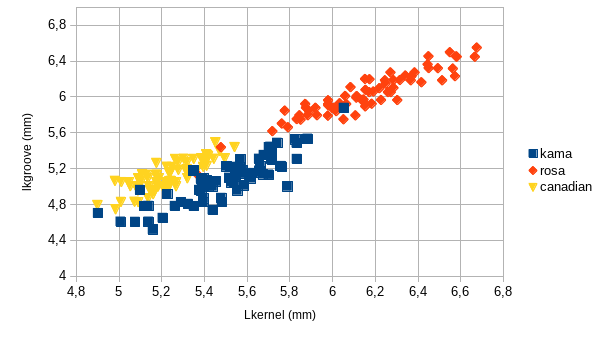
\includegraphics[scale=0.9]{figs/grafico_NB_cluster1_lkernel_lkgroove_seeds.png}
        \caption{Gráfico da disposição de elementos da Base Seeds entre os eixos \textbf{Lkernel} e \textbf{lkgroove}} \label{fig:grafico_NB_cluster1_lkernel_lkgroove_seeds}
\end{figure}


Na situação da figura \ref{fig:grafico_NB_cluster1_lkernel_lkgroove_seeds}, pode-se perceber que o grupo \textit{kama} (\textit{cluster} 1) contém alguns erros, pois logo no início da faixa $ (Lkernel, ] 5.357 \sim  5.826 ]) $ é fácil visualizar que alguns dados ficam fora da faixa, indicando que não estão sendo representados pelo rótulo, ocasionando os erros, contudo é possível ter uma impressão generalizada de todos os registros que o rótulo representa através dos valores de intervalo do rótulo. 

A figura \ref{fig:grafico_NB_cluster1_2_wkernel_lkgroove_seeds} também apresenta a base Seeds, distinguindo os grupos pelas formas geométricas: quadrados (\textit{Kama}), losango (\textit{Rosa}) e triângulos (\textit{Canadian}), mas com uma relação entre \textbf{lkgroove} e \textbf{wkernel} que fazem parte dos resultados de rotulação do Naive Bayes no \textit{cluster} 2 $r_{c_2}=\{ (lkgroove, ] 5.791 \sim  6.55]) \} $ e no \textit{cluster} 3 $r_{c_3}=\{ (wkernel, [2.63 \sim  3.049])\}$.
 
\begin{figure}[h!]
        \centering
        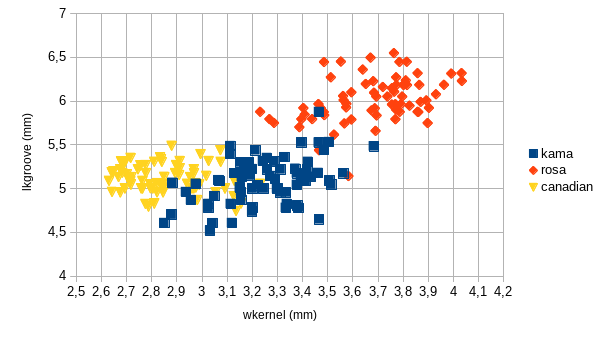
\includegraphics[scale=0.9]{figs/grafico_NB_cluster1_2_wkernel_lkgroove_seeds.png}
        \caption{Gráfico da disposição de elementos da Base Seeds entre os eixos \textbf{Lkernel} e \textbf{lkgroove}} \label{fig:grafico_NB_cluster1_2_wkernel_lkgroove_seeds}
\end{figure}
 

O atributo \textbf{lkgroove} faz parte do rótulo encontrado no grupo \textit{Rosa} (\textit{cluster} 2) pelo Naive Bayes, representado no gráfico pelo eixo Y da figura \ref{fig:grafico_NB_cluster1_2_wkernel_lkgroove_seeds}   e sua faixa de dados é de fácil visualização no gráfico. Os valores do eixo Y acima de 5.791 até 6.55 são representados por  ${r_{c_2}}$ do grupo \textit{Rosa}, figurado pelo losango no gráfico da figura \ref{fig:grafico_NB_cluster1_2_wkernel_lkgroove_seeds}. Já o ${r_{c_3}}$ possui o atributo \textbf{wkernel}, representado no gráfico no eixo X, possuindo uma faixa de dados a partir de 2.63 até 3.049 e através desse intervalo é possível notar que há alguns dados não pertencentes ao ${r_{c_3}}$ do grupo \textit{Canadian}. Com o gráfico fica fácil perceber que, na disposição das amostras, o grupo que mais se mistura é o \textit{Kama}, implicando também na menor acurácia entre os rótulos. No outro gráfico, figura \ref{fig:grafico_CART_KNN_SEEDS_perimetro_lkgroove}, são relacionados dois eixos X e Y com os atributos \textbf{perimetro} e \textbf{lkgroove}, respectivamente, e através desse plano cartesiano é possível identificar todos os grupos da base Seeds. Os dois algoritmos CART e KNN possuem os mesmos resultados de rotulação para os três grupos mediante os dois atributos que estão representados no gráfico. Dessa forma, com essa amostra de dados é possível representar o espaço de dados dos rótulos encontrados em cada algoritmo. 

\begin{figure}[h!]
        \centering
        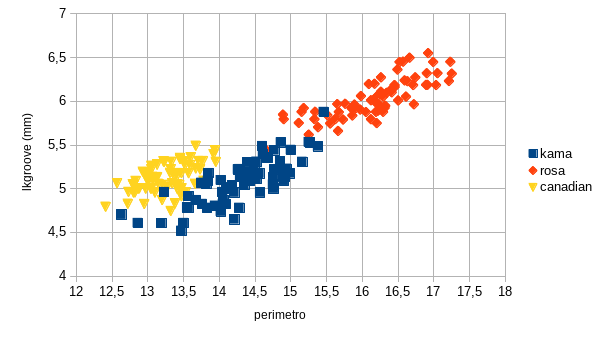
\includegraphics[scale=0.9]{figs/grafico_CART_KNN_SEEDS_perimetro_lkgroove.png}
        \caption{Gráfico da disposição de elementos da Base Seeds entre os eixos \textbf{Lkernel} e \textbf{lkgroove}} \label{fig:grafico_CART_KNN_SEEDS_perimetro_lkgroove}
\end{figure}


Os elementos do rótulo $r_{c_1}=\{ (perimetro, ]13.73 \sim 15.18]) \} $ representam o grupo \textit{Kama}, que estão simbolizados por quadrados no gráfico, e através do atributo \textbf{perimetro} no intervalo de ]13.73 até 15.78] consegue-se visualizar no gráfico a amostra que o rótulo representa do \textit{cluster} 1 (\textit{Kama}), como também alguns dados que não estão neste intervalo configurando os erros. 


No \textit{cluster} 2 (\textit{Rosa}) figurando no gráfico como um losango, pode-se perceber, através de seu rótulo $r_{c_2}=\{ (lkgroove, ] 5.791 \sim  6.55]) \}$, que o atributo lkgroove e seu intervalo estão bem definidos no gráfico. Qualquer valor no eixo Y no intervalo, a partir de 5.6791 até 6.55, é representado pelo rótulo ${r_{c_2}}$, mas mesmo com alguns erros visíveis na amostra, esse grupo foi o que ficou melhor delineado no gráfico e de fácil visualização para comprovar a representatividade dos rótulos encontrados pelos algoritmos CART e KNN. Já no cluster 3, Canadian, não é diferente mediante o rótulo encontrado pelos dois algoritmos $r_{c_3}=\{ (perimetro, [12.41 \sim  13.73])\}$. A partir da faixa do ${r_{c_3}}$ no atributo \textbf{perimetro}, as amostras representadas iniciam em 12.41 até 13.73, mas, mesmo no valor final do intervalo, em que se pode encontrar alguns erros, é possível mostrar que o ${r_{c_3}}$ consegue representar o grupo \textit{Canadian}. 

\section{Base de Dados 2 - Iris - Identificação de Tipos de Plantas}

A base de dados Iris pertence à UCI Machine Learning, já usada em trabalhos como \citeonline{Lopes2016,Filho2015}, e utilizada em reconhecimento de padrões de plantas por lidar com classes bem definidas, pois contém 3 classes de 50 instâncias cada, totalizando 150 registros de amostras de plantas. A base possui amostras com 3 tipos \cite{FISHER1936}: 

\begin{itemize}[noitemsep]
 \item 50 elementos da classe \textit{Iris-setosa} ;
 \item 50 elementos da classe \textit{Iris-versicolor};
 \item 50 elementos da classe \textit{Iris-virginica}.
\end{itemize}

% Os atributos correspondentes são comprimento da sepala - SL, largura da sepala - SW, comprimento da pétala - PL e largura da pétala - PW, e através dessas características há uma classificação para dizer se o tipo de planta é: \textit{Iris-setosa}, \textit{Iris-versicolor} e \textit{Iris-virginica}.
% 
% Seguindo a análise, semelhante a da base de dados anterior, foram realizados testes utilizando os algoritmos Naive Bayes, CART e KNN e seus resultados depositados em tabelas divididas em colunas no mesmo formato das anteriores: \textbf{Cluster}, \textbf{Rótulo}, \textbf{Relevância}, \textbf{Fora da Faixa} e \textbf{Acurácia Parcial}. Os \textit{clusters} são dispostos em números correspondentes a seguinte sequência: (1) \textit{Iris-setosa}, (2) \textit{Iris-versicolor} e (3) \textit{Iris-virginica}.
 
Os atributos correspondentes são: comprimento da sepala - SL, largura da sepala - SW, comprimento da pétala - PL e largura da pétala - PW, e através dessas características há uma classificação para dizer se o tipo de planta é: \textit{Iris-setosa}, \textit{Iris-versicolor} e \textit{Iris-virginica}. 

Seguindo a análise, semelhante à da base de dados anterior, foram realizados testes utilizando-se os algoritmos Naive Bayes, CART e KNN e seus resultados depositados em tabelas divididas em colunas no mesmo formato das anteriores: \textbf{Cluster}, \textbf{Rótulo}, \textbf{Elementos Fora da Faixa} e \textbf{Acurácia Parcial}. Os \textit{clusters} são dispostos em números correspondentes à seguinte sequência: (1) \textit{Iris-setosa}, (2) \textit{Iris-versicolor} e (3) \textit{Iris-virginica}.
 
 
Para gerar os resultados da aplicação do algoritmo na base de dados, foi definido o método de discretização tipo EWD (seção \ref{cap:refTeor:subsec:ewd}), a divisão em três faixas de valores ${R = 3}$ para todos os atributos e inserido o valor de variação ${V=0\%}$. 

\subsection{Rotulação através do algoritmo Naive Bayes} \label{cap:resultados:ssec:iris:nb}

Através da tabela \ref{tab:rot:iris:nb}  são exibidos os resultados da rotulação de dados de todos os grupos: \textit{cluster} 1 (\textit{Iris-setosa}), \textit{cluster} 2 (\textit{Iris-versicolor}) e \textit{cluster} 3 (\textit{Iris-virginica}). O Naive Bayes encontrou o mesmo atributo para cada rótulo, mas os intervalos foram diferentes, assegurando-se que os rótulos se tornassem distintos. 
 
\begin{table}[!ht]
\centering
\caption{Resultado da aplicação do algoritmo Naive Bayes}
\label{tab:rot:iris:nb}
\scalebox{0.8}{
\begin{tabular}{llccc} \hline \hline
 
\multicolumn{1}{c}{\cellcolor[HTML]{FFFFFF}} & \multicolumn{2}{c}{Rótulos}                & \multicolumn{1}{r}{}               & \\ \cline{2-3}
Cluster                                      & Atributos      & \multicolumn{1}{c}{Faixa} &  Elementos Fora da Faixa & Acurácia Cluster(\%)\\ \hline \hline                                             
1                                            & petalwidth     & [ 0.1 $\sim$  0.9 ]       &  0 & 100\% \\  \hline
2                                             & petalwidth    & ] 0.9 $\sim$  1.7 ]       &  2 & 94\% \\ \hline
3                                            & petalwidth     & ] 1.7 $\sim$  2.5 ]       &  4 & 92\% \\ \hline \hline
\end{tabular}}
\end{table}



O fato de os rótulos apresentarem o mesmo atributo implica que o algoritmo em seus testes, na técnica de correlacionamento, obteve a maior taxa de acerto no atributo \textbf{petalwidth} em todos os \textit{clusters}, isso não implica que as taxas de acerto são as mesmas em cada \textit{cluster}, e sim, que são as maiores.  Esses valores são armazenados na tabela de atributos importantes e expõe as taxas de acerto entre atributos, e através dela que é escolhido o atributo para rótulo. 
% 
% \begin{table}[!h]
% \centering
% \caption{Matriz de Atributos Importantes do algoritmo Naive Bayes na base Iris}
% \label{tab:execucoes:iris:cart}
% \scalebox{0.8}{
% \begin{tabular}{|cl|c|c|c|c|}
%         \hline \hline
%                      &   & \multicolumn{4}{c|}{Atributos}                                               \\ \cline{3-6} 
%        \multicolumn{1}{|l}{}                             &   & sepallength   & sepalwidth     & petallength    & petalwidth     \\ \hline
%         \multicolumn{1}{|c|}{}                           & 1 & 14   & 16     & 26   & \textbf{42}       \\ \cline{2-6} 
%         \multicolumn{1}{|c|}{}                           & 2 & 16 & 12   & 14  & \textbf{36}     \\ \cline{2-6} 
%         \multicolumn{1}{|c|}{\multirow{-3}{*}{Clusters}} & 3 & 14 & 16   & 14  & \textbf{20}     \\ \hline
%       \end{tabular}}
% \end{table}    


Os rótulos com o algoritmo Naive Bayes na base de dados \textbf{Iris} são dados abaixo:

% A tabela \ref{tab:execucoes:iris:cart} mantém os resultados de correlacionamento entre os atributos e quando ela está toda preenchida é realizada uma varredura por linha para saber qual o maior valor, servindo para indicar qual o atributo será o rótulo; desta forma, como todos os maiores números estão na coluna do atributo \textbf{petalwidth}, este atributo é o rótulo de cada \textit{cluster}. Os rótulos com o algoritmo Naive Bayes na base de dados Iris são dados abaixo: 

\begin{itemize}[noitemsep]
 \item ${r_{c_1}=\{ (petalwidth,[ 0.1 \sim 0.9 ] ) \} }$  
 \item ${r_{c_2}=\{ (petalwidth, ] 0.9 \sim 1.7]) \} }$
 \item ${r_{c_3}=\{ (petalwidth, ] 1.7 \sim 2.5 ]) \} }$
\end{itemize}

\subsection{Rotulação através do algoritmo Classification and Regression Trees - CART} \label{cap:resultados:ssec:iris:cart}


A aplicação do algoritmo CART na base de dados Iris gerou a tabela \ref{tab:rot:iris:cart} como resultado e, ao examiná-la, pode-se observar uma semelhança com a rotulação do algoritmo anterior.

\begin{table}[!ht]
\centering
\caption{Resultado da aplicação do algoritmo CART}
\label{tab:rot:iris:cart}
\scalebox{0.8}{
\begin{tabular}{llccc} \hline \hline
 
\multicolumn{1}{c}{\cellcolor[HTML]{FFFFFF}} & \multicolumn{2}{c}{Rótulos}                & \multicolumn{1}{r}{}               & \\ \cline{2-3}
Cluster                                      & Atributos      & \multicolumn{1}{c}{Faixa} & Elmentos Fora da Faixa & Acurácia Cluster(\%)\\ \hline \hline                                             
1                                            & petalwidth     & [ 0.1 $\sim$  0.9 ]       &  0 & 100\% \\  \hline
2                                             & petalwidth    & ] 0.9 $\sim$  1.7 ]       &  2 & 94\% \\ \hline
3                                            & petalwidth     & ] 1.7 $\sim$  2.5 ]       &  4 & 92\% \\ \hline \hline
\end{tabular}}
\end{table}


Ao se analisar a tabela, percebe-se a importância do atributo \textbf{petalwidth} para essa base, pois este tem participação nos três \textit{clusters}:\textit{Iris-setosa}, \textit{Iris-versicolor}, \textit{Iris-virginica} e também diferenciados apenas pelo intervalo de dados. Este resultado, para um especialista, ajudaria em uma tomada de decisão, pois a partir da leitura destes rótulos, para qualquer novo registro, basta verificar o valor da largura da pétala (\textbf{petalwidth}) para poder classificá-la em algum grupo.

Seguem abaixo os rótulos na base de dados \textbf{Iris} aplicado pelo algoritmo CART:
\begin{itemize}[noitemsep]
 \item ${r_{c_1}=\{ (petalwidth,[ 0.1 \sim 0.9 ] ) \} }$  
 \item ${r_{c_2}=\{ (petalwidth, ] 0.9 \sim 1.7]) \} }$
 \item ${r_{c_3}=\{ (petalwidth, ] 1.7 \sim 2.5 ]) \} }$
\end{itemize}


\subsection{Rotulação através do algoritmo  K-Nearest Neighbor - KNN} \label{cap:resultados:ssec:iris:knn}

No resultado da rotulação utilizando-se KNN, constatam-se os mesmos rótulos dos dois algoritmos Naive Bayes e CART, mantendo-se os mesmos valores também para as outras colunas:

\begin{table}[!ht]
\centering
\caption{Resultado da aplicação do algoritmo KNN}
\label{tab:rot:iris:cart}
\scalebox{0.8}{
\begin{tabular}{llccc} \hline \hline
 
\multicolumn{1}{c}{\cellcolor[HTML]{FFFFFF}} & \multicolumn{2}{c}{Rótulos}                & \multicolumn{1}{r}{}               & \\ \cline{2-3}
Cluster                                      & Atributos      & \multicolumn{1}{c}{Faixa} &  Elementos Fora da Faixa & Acurácia Cluster(\%)\\ \hline \hline                                             
1                                            & petalwidth     & [ 0.1 $\sim$  0.9 ]       &  0 & 100\% \\  \hline
2                                             & petalwidth    & ] 0.9 $\sim$  1.7 ]       & 2 & 94\% \\ \hline
3                                            & petalwidth     & ] 1.7 $\sim$  2.5 ]       &  4 & 92\% \\ \hline \hline
\end{tabular}}
\end{table}

Seguem abaixo os rótulos na base de dados \textbf{Iris} aplicado pelo algoritmo KNN:
\begin{itemize}[noitemsep]
 \item ${r_{c_1}=\{ (petalwidth,[ 0.1 \sim 0.9 ] ) \} }$  
 \item ${r_{c_2}=\{ (petalwidth, ] 0.9 \sim 1.7]) \} }$
 \item ${r_{c_3}=\{ (petalwidth, ] 1.7 \sim 2.5 ]) \} }$
\end{itemize}

\subsection{Avaliação da rotulação através de algoritmos supervisionados na base de dados Iris} \label{cap:resultados:ssec:compalgoritmos:iris}

Os resultados dos algoritmos na criação dos rótulos, nesta base de dados, foram bastante concisos entre eles, pois cada rótulo possui somente um atributo e faixa de valor representando o grupo e os três algoritmos Naive Bayes, CART e KNN tiveram exatamente os mesmos rótulos em todos os três \textit{clusters}. 

Uma forma de comprovar a qualidade do rótulo e mostrar que de fato ele cumpre seu papel de identificar o grupo, é colocar em prática um exemplo que pode ser visto na figura \ref{fig:grafico_iris_petalwidth_petallength_BrOf}. Para essa análise, o gráfico exibe a relação de dois atributos representados pelos eixos X e Y, facilitando a visualização do comportamento dos três grupos: \textit{Iris-setosa}, \textit{Iris-versicolor} e \textit{Iris-viginica}.

\begin{figure}[h!]
        \centering
        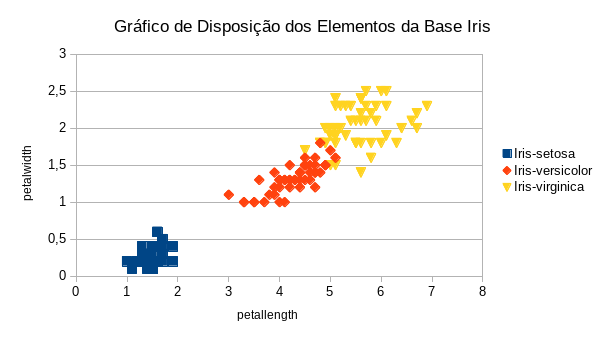
\includegraphics[scale=0.9]{figs/grafico_iris_petalwidth_petallength_BrOf.png}
        \caption{Gráfico da disposição de elementos da Base Iris entre os eixos \textbf{petallength} e \textbf{petalwidth}} \label{fig:grafico_iris_petalwidth_petallength_BrOf}
\end{figure}


Todos os algoritmos, Naive Bayes, CART e KNN, encontraram os mesmos rótulos em todos os clusters da Iris e ao se analisar o gráfico, o \textit{cluster} 1 (\textit{Iris-setosa}), é possível perceber uma relação bem definida entre os demais grupos, pois todos os elementos que possuem largura da pétala (\textit{petalwidth}) variando de 0.1 até 0.9 participam do grupo \textit{Iris-setosa}, portanto, esse rótulo comprovadamente representa este grupo. Analisando-se os outros grupos através do gráfico da figura \ref{fig:grafico_iris_petalwidth_petallength_BrOf}, percebe-se que a amostra de dados dos grupos \textit{Iris-versicolor} e \textit{Iris-virginica} contém elementos que se misturam, não deixando um ponto de corte tão preciso quanto o da Iris-setosa e isso acaba por também ocasionar ao rótulo alguns erros identificados nos \textit{clusters} 1 e 2. 
\newpage
\section{Base de Dados 3 - Glass - Identificação de Tipos de Vidros}\label{cap:resultados:ssec:iris}


A base de dados dos tipos de vidro ficou conhecida através de estudos do Dr. Vina Spiehler, Ph.D. da DABFT Diagnostic Products Corporation,  que conduziu pesquisas e testes de comparação em seu sistema baseado em regras, determinando se o tipo de vidro era temperado ou não. Institutos de investigação criminológica motivaram os estudos de classificação de tipos de vidro, porque, em uma cena de crime, uma classificação de tipos de vidro corretamente identificada pode ser utilizada como prova, ajudando diretamente na investigação \cite{Evett:1989}.

A base de vidros possui um total de 214 instâncias, caracterizados por 9 atributos: índice de refração (RI) e os demais atributos correspondentes à porcentagem do óxido no Sódio (Na), Magnésio (Mg), Alumínio (Al), Silício (Si), Potássio (K), Cálcio (Ca), Bário (Ba) e Ferro (Fe).

Os tipos de vidro (atributo classe) foram divididos em 7 grupos distintos:
\begin{itemize} [noitemsep]
 \item janelas de construção - vidro temperado: 70 registros
 \item janelas de construção - vidro não-temperado: 76 registros
 \item janelas de veículos - vidro temperado: 17 registros
 \item janelas de veículos - vidro não-temperado: 0 registro
 \item recipientes: 13 registros
 \item louças de mesa: 9 registros
 \item lâmpadas: 29 registros 
\end{itemize}


Essa é uma base de dados diferente das demais por possuir mais grupos e, especificamente, o grupo de janelas de veículos - vidro não-temperado, que não possuem amostras de dados para exemplificar. Nos resultados dos rótulos exibidos nas tabelas adiante a coluna \textit{Cluster}, que exibe uma sequência numérica dos grupos, não contemplará o grupo janelas de veículos - vidro não-temperado, pois não há exemplos de dados para definir o grupo, ficando somente seis grupos determinados na seguinte sequência : (1) janelas de construção - vidro temperado, (2) janelas de construção - vidro não-temperado, (3) janelas de veículos - vidro temperado, (4) recipientes , (5) louças de mesa e (6) lâmpadas. 


Nos testes desenvolvidos nesta pesquisa, os valores de referência foram ${R=4}$ para o número de faixas. O método de discretização e também a variância ${V}$ sofreram alterações nas execuções nos próprios algoritmos para melhorar seus resultados. O que mais diferenciou os resultados desta base foi a necessidade de se utilizarem valores de ${V}$ bastante altos para poder conseguir criar rótulos distintos. 

\subsection{Rotulação através do algoritmo Naive Bayes} \label{cap:resultados:ssec:glass:nb}

 

Na aplicação desse algoritmo, as melhores configurações para rotulação foram através do método EWD de discretização e a variação  ${V=77\%}$, que influencia diretamente nas escolhas dos atributos. 

 A tabela \ref{tab:rot:glass:nb}  apresenta os seis clusters nas ordens sequenciais:(1) janelas de construção - vidro temperado, (2) janelas de construção - vidro não-temperado, (3) janelas de veículos - vidro temperado, (4) recipientes , (5) louças de mesa e (6) lâmpadas, e junto a coluna Cluster segue a sequência da coluna Rótulos (Atributo/Faixa), com os erros (Elementos Fora da Faixa) e Acurácia Parcial indicada para cada atributo junto ao cluster. 
 

\begin{table}[!ht]
\centering
\caption{Resultado da aplicação do algoritmo Naive Bayes}
\label{tab:rot:glass:nb}
\scalebox{0.8}{
\begin{tabular}{llccc} 
\hline \hline
 
\multicolumn{1}{c}{\cellcolor[HTML]{FFFFFF}} & \multicolumn{2}{c}{Rótulos}                & \multicolumn{1}{r}{}               & \\ \cline{2-3}
Cluster                                      & Atributos      & \multicolumn{1}{c}{Faixa} &  Elementos Fora da Faixa & Acurácia Parcial(\%)\\ \hline \hline
                                             & Ba     & [ 0.0 $\sim$  0.7875 ]   &  0 & 100\% \\  
\multirow{-2}{*}{1}                          & Fe    & [ 0.0 $\sim$  0.1275  ]   &  15 & 78.6\% \\  \hline
                                             & Mg    & ] 3.3675 $\sim$  4.49 ]   &  25 & 68\%\\ 
                                             & K     & [ 0.0 $\sim$  1.5525 ]     &  0  & 100\% \\  
                                            & Ba     & [ 0.0 $\sim$  0.7875 ]    &  1  & 98.7\% \\  
\multirow{-4}{*}{2}                          & Fe    & [ 0.0 $\sim$  0.1275 ]    &  23 & 69.8\% \\  \hline
                                            & Na     & ]12.3925 $\sim$  14.055 ] &  3  & 82.4\% \\ 
                                            & Ba     & [ 0.0 $\sim$  0.7875 ]    &  0  & 100\% \\  
\multirow{-3}{*}{3}                          & Fe    & [ 0.0 $\sim$  0.1275 ]    &  3  & 82.4\% \\  \hline
                                             & Mg    & [ 0.0 $\sim$  1.1225 ]    &  5  & 61.6\%\\ 
                                             & Al    & ] 1.0925 $\sim$  1.895]      & 1 4  & 69.3\%\\
                                            & K     & [  0.0 $\sim$  1.5525 ]    &  3  & 77\% \\ 
                                            & Ba     & [ 0.0 $\sim$  0.7875 ]    &  1  & 92.4\% \\  
\multirow{-5}{*}{4}                          & Fe    & [ 0.0 $\sim$  0.1275 ]    &  2  & 84.7\% \\  \hline                                            
                                            & K     & [ 0.00 $\sim$ 1.5525 ]     & 0 & 100\% \\ 
                                            & Ba     & [ 0.0 $\sim$  0.7875 ]    &  0 & 100\% \\  
\multirow{-3}{*}{5}                         & Fe    & [ 0.0 $\sim$  0.1275 ]     &  0 & 100\% \\  \hline
                                            & RI     & [1.511150 $\sim$  1.516845 ] &  11  & 62.1\% \\ 
                                            & Na     & ]14.055 $\sim$  15.7175 ] &  6  & 79.4\% \\ 
                                             & Mg    & [ 0.0 $\sim$  1.1225 ]    & 6  & 79.4\%\\ 
                                             & Al    & ] 1.895 $\sim$  2.6975]      &  11  & 62.1\%\\
                                            & Si    & ] 72.61 $\sim$  74.01]      &  6  & 79.4\%\\
                                            & K     & [  0.0 $\sim$  1.5525 ]    &  2  & 93.2\% \\ 
                                            & Ca     & [ 8.12 $\sim$ 10.81 ]    &  3  & 89.7\% \\ 
                                            & Ba     & [ 0.0 $\sim$  0.7875 ]    &  15  & 48.3\% \\  
\multirow{-3}{*}{6}                         & Fe    & [ 0.0 $\sim$  0.1275 ]     &  0  & 100\% \\  \hline

\end{tabular}
}
\end{table}



Analisando-se a tabela \ref{tab:rot:glass:nb} percebe-se, através dos rótulos, que entre os \textit{clusters} 1 ao 6 o atributo \textbf{Ba} e \textbf{Fe} se repetem. No caso do resultado desse algoritmo aconteceu da tabela de atributos importantes coincidir estes dois atributos junto com as mesmas faixas nos \textit{clusters} 1, 3 e 5. Dessa forma, isso configura uma ambiguidade de rótulos entre três grupos, \textit{i.e.}, o mesmo rótulo está representando três grupos ao mesmo tempo. A solução para evitar a ambiguidade entre rótulos é agregar mais atributos de menores taxas de acerto do algoritmo, através da variância ${V}$ até que os rótulos se tornem únicos por grupo. 


Sabe-se que, ao incluir atributos de com menores taxas de acerto nos rótulos para deixá-los únicos, isso resulta na diminuição da acurácia média do grupo, porém essa diminuição de confiança do rótulo é necessária para manter a representatividade dele. Essa situação ocorreu com o \textit{cluster} 6, que possuiu umas das menores acurácias médias por possuir todos os atributos como rótulo, e isso devido a dois fatores: i) os valores da tabela de atributos importantes, que mantém armazenados as taxas de acerto do algoritmo, contêm valores baixos; ii) o valor da variância ser maior que os valores armazenados na tabela do respectivo \textit{cluster}. Ao acontecer esses dois fatores acaba por  resultar em um rótulo com todos os atributos. 

Considerando-se a tabela \ref{tab:rot:glass:nb}, o \textit{cluster} 5 foi o único, mesmo com ${V=77\%}$, a apresentar um rótulo com valor de 100\% na acurácia média do grupo. As menores acurácias médias, por grupo, foi do \textit{cluster} 4 (\textbf{recipientes}) e \textit{cluster} 6 (\textbf{lâmpadas}), com 77\% e 77.06\% respectivamente. 

%Em análise a um fato que ocorreu em específico no \textit{cluster} 6, foi que o maior valor da taxa de acerto do Naive Bayes no \textit{cluster} é do atributo \textbf{Mg} de 68\%, visto que a variância é igual a ${V=77\%}$, e tem o efeito de adicionar todos os atributos que possuem valores abaixo dele no rótulo, dessa forma o atributo \textbf{Na} com relevância de 0\% também é adicionado ao rótulo. Uma vez que o atributo faz parte do rótulo é calculado  qual  faixa de valor, do atributo, possui mais elementos. Então o motivo de um atributo que tem 0\% de relevância, entre atributos, e ter 86.3\% de acurácia é justificado pelo fato de contabilizar os registros que possuem valores de \textbf{Na} no intervalo ${]14.055 \sim 15.7175 ]}$. 

%Em análise a um fato que ocorreu em específico no \textit{cluster} 6, verificou-se que o maior valor de relevância do \textit{cluster} é do atributo \textbf{Mg}, de 68\%, sendo menor que o valor de  variância igual a ${V=77\%}$. Uma vez que a variáncia tenha um valor maior do que relevância do atributo do cluster, então todos os atributos que possuem o valor abaixo da variância serão adicionados ao rótulo; dessa forma, o atributo \textbf{Na}, com relevância de 0\%, também é adicionado ao rótulo, e calculada qual faixa de valor do atributo possui mais elementos. Então, uma vez que o atributo faz parte do rótulo, irá ser contabilizado o número de registros que estejam entre o intervalo do atributo e calculado sua acurácia.
% 
% Outra forma de explicar o valor de variância  ${V=}$ é verificar na tabela \ref{tab:execucoes:glass:nb} (matriz de atributos importantes) os valores correspondentes aos \textit{clusters} que possuem maiores números, pois esta contêm valores em porcentagem do quanto cada atributo é bem correlacionado com os demais, logo, quanto maior for o valor mais bem correlacionado é o atributo. Cada linha da tabela corresponde a um cluster e as colunas os atributos.
% 
% \begin{table}[!h]
% \centering
% \caption{Matriz de Atributos Importantes do algoritmo Naive Bayes na base Glass}
% \label{tab:execucoes:glass:nb}
% \scalebox{0.7}{
% 
%    %\small\addtolength{\tabcolsep}{-2pt} 
%     \begin{tabular}{|cl|c|c|c|c|c|c|c|c|c|}
%         \hline \hline
%             {\tiny }     &   & \multicolumn{9}{c|}{\tiny Atributos}                                               \\ \cline{3-11} 
%        \multicolumn{1}{|l}{}    &   & RI    & Na    & Mg  & Al   & Si   & K   & Ca   & Ba  & Fe             \\ \hline
%         \multicolumn{1}{|c|}{}  & 1 & 8.5714 & 7.1429  & 4.2857 & 4.2857 & 8.5714 & 10.0 & 0 & 91.4286 & 58.5714 \\ \cline{2-11} 
%         \multicolumn{1}{|c|}{}  & 2 & 2.6316  &  3.9474  &  14.4737  &  3.9474  &  0  & 11.8421  & 2.6316 & 85.5263  &  51.3158   \\ \cline{2-11} 
%         \multicolumn{1}{|c|}{}  & 3 &  11.7647  &  17.6471  & 11.7647  &  0  &  0  & 5.8824  &  11.7647 & 94.1176  &  70.5882   \\ \cline{2-11}
%         \multicolumn{1}{|c|}{}  & 4 &  0  &  0  &  46.1538  &  15.3846  &  0  &  15.3846  &  0  &  84.6154  &  84.6154  \\ \cline{2-11}
%         \multicolumn{1}{|c|}{}  & 5 &  0  &  0  &  11.1111  &  0  &  0   & 100.00 &  0  &  100.00 & 100.00  \\ \cline{2-11}
%         \multicolumn{1}{|c|}{\multirow{-3}{*}{\tiny Clusters}} & 6 &  6.8966  &  0  &  68.9655  &  6.8966  &  10.3448  &  48.2759  &  0  &  10.3448  & 58.6207  \\ \hline
%         
%         
%     \end{tabular}
% 
% }
% \end{table}  
% 
% Em análise dos resultados da execução do Naive Bayes os atributos \textbf{Ba} e \textbf{Fe} são os 
% que aparecem em todos os rótulos indicando uma importância desses elementos nos grupos, que pode também ser percebido através dos altos valores de correlacionamento na tabela \ref{tab:execucoes:glass:nb}. Neste resultado observa-se que o cluster 6 acabou por ter um rótulo o qual todos os atributos estão selecionados, ou seja, fazem parte do rótulo, esse efeito foi causa da variância ${V}$ que atingiu um número maior, em relação ao resultado da diferença entre, o maior e menor valor  da linha respectiva a do cluster 6 da tabela \ref{tab:execucoes:glass:nb}. Dito isto, a variável cumpre seu papel de não deixar que rótulos repetidos existam.
% acurácia media p/ grupo
% cluster1=89.3
% cluster2=84.125
% cluster3=88.2
% cluster4=77
% cluster5 = 100
% cluster6=77.066



De acordo com a aplicação do Naive Bayes na base de dados \textbf{Glass} os rótulos são os seguintes:
\begin{itemize}[noitemsep]
 \item ${r_{c_1}=\{ (Ba,[ 0.0 \sim 0.7875 ] ),(Fe,[ 0.0 \sim 0.1275 ] ) \} }$  
 \item ${r_{c_2}=\{ (Mg,] 3.3675 \sim  4.49 ] ),(K,[ 0.0 \sim 1.5525 ] ),(Ba,[ 0.0 \sim 0.7875 ] ),}$
 
 ${(Fe,[ 0.0 \sim 0.1275 ] ) \} }$
 \item ${r_{c_3}=\{ ((Na,]12.3925 \sim 14.055 ] ),(Ba,[ 0.0 \sim 0.7875 ] ),(Fe,[ 0.0 \sim 0.1275 ] )  \} }$  
 \item ${r_{c_4}=\{ (Mg,[ 0.0 \sim  1.1225 ] ),(Al,] 1.0925 \sim 1.895 ] ), (K,[ 0.0 \sim 1.5525 ] ),}$

 ${ (Ba,[ 0.0 \sim 0.7875 ] ),(Fe,[ 0.0 \sim 0.1275 ] ) \} }$
 \item ${r_{c_5}=\{  (K,[ 0.0 \sim 1.5525 ]  ),(Ba,[ 0.0 \sim 0.7875 ] ), (Fe,[ 0.0 \sim 0.1275 ] )\} }$
 \item ${r_{c_6}=\{ (RI,[ 1.511150 \sim  1.516845  ] ),(Na,]14.055 \sim 15.7175 ] ),  (Mg,[ 0.0 \sim  1.1225  ] ), }$
 
 ${ (Al,] 1.895 \sim 2.6975 ] ), (Si,] 72.61 \sim 74.01 ] ),  }$
 
 ${ (K,[ 0.0 \sim 1.5525] ),(Fe,[ 0.0 \sim 0.1275 ] ) \} }$
\end{itemize}


\subsection{Rotulação através do algoritmo Classification and Regression Trees - CART} \label{cap:resultados:ssec:glass:cart}

%Na execução do CART foi aplicado o método de discretização EWD e uma mudança no valor da variância ${V=6\%}$ para evitar a ambiguidade dos clusters 1 e 3. 

Por meio de testes foi descartada a utilização do método de discretização EFD e adotado o EWD, em virtude da diminuição de erros por atributo em comparação ao outro método, e na divisão de faixas foi mantido ${R=4}$. Quanto à variável ${V}$, houve alteração em relação ao algoritmo anterior, mas mesmo assim manteve-se um valor alto com  ${V=71\%}$, em razão do número de \textit{clusters} com rótulos iguais. Este aumento da variável ${V}$ tem influência direta, diminuindo a acurácia média do cluster, embora seja justificado esse aumento de ${V}$ devido não poder haver repetição dos rótulos nos \textit{clusters}. 

A execução do CART obteve os resultados apresentados na tabela \ref{tab:rot:glass:cart}.

\begin{table}[!ht]
\centering
\caption{Resultado da aplicação do algoritmo CART}
\label{tab:rot:glass:cart}
\scalebox{0.8}{
\begin{tabular}{llccc} 
\hline \hline
 
\multicolumn{1}{c}{\cellcolor[HTML]{FFFFFF}} & \multicolumn{2}{c}{Rótulos}                & \multicolumn{1}{r}{}               & \\ \cline{2-3}
Cluster                                      & Atributos      & \multicolumn{1}{c}{Faixa} & Elementos Fora da Faixa & Acurácia Parcial(\%)\\ \hline \hline
                                             & Ba     & [ 0.0 $\sim$  0.7875 ]   &  0 & 100\% \\  
\multirow{-2}{*}{1}                          & Fe    & [ 0.0 $\sim$  0.1275  ]   &  15 & 78.6\% \\  \hline
                                             & Mg    & ] 3.3675 $\sim$  4.49 ]   &  25 & 68\%\\ 
                                            & Ba     & [ 0.0 $\sim$  0.7875 ]    &  1  & 98.7\% \\  
\multirow{-3}{*}{2}                          & Fe    & [ 0.0 $\sim$  0.1275 ]    &  23 & 69.8\% \\  \hline
                                            & K     & [ 0.0 $\sim$  1.5525 ]     &  0  & 100\% \\ 
                                            & Ba     & [ 0.0 $\sim$  0.7875 ]    &  0  & 100\% \\  
\multirow{-3}{*}{3}                          & Fe    & [ 0.0 $\sim$  0.1275 ]    &  3  & 82.7\% \\  \hline
                                             & Mg    & [ 0.0 $\sim$  1.1225 ]    &  5  & 61.6\%\\ 
                                             & Al    & ] 1.43 $\sim$  1.83]      &  4  & 69.3\%\\
                                            & K     & [  0.0 $\sim$  1.5525 ]    &  3  & 77\% \\ 
                                            & Ba     & [ 0.0 $\sim$  0.7875 ]    &  1  & 92.4\% \\  
\multirow{-5}{*}{4}                          & Fe    & [ 0.0 $\sim$  0.1275 ]    &  2  & 84.7\% \\  \hline
                                            & Mg    & [ 0.0 $\sim$  1.1225 ]     &  5  & 44.5\% \\ 
                                            & K     & [ 0.00 $\sim$ 1.5525 ]     &  0 & 100\% \\ 
                                            & Ba     & [ 0.0 $\sim$  0.7875 ]    &  0 & 100\% \\  
\multirow{-4}{*}{5}                         & Fe    & [ 0.0 $\sim$  0.1275 ]     &  0 & 100\% \\  \hline
                                            & Mg    & [ 0.0 $\sim$  1.1225 ]     &  6  & 79.4\% \\ 
                                            & K     & [ 0.0 $\sim$ 1.5525 ]      &  2  & 93.2\% \\ 
\multirow{-3}{*}{6}                         & Fe    & [ 0.0 $\sim$  0.1275 ]     &  0  & 100\% \\  \hline

\end{tabular}
}
\end{table}


As acurácias parciais exibidas na tabela \ref{tab:rot:glass:cart} foram bem diversificadas, bem como o número de atributos por rótulo, embora mais uma vez os elementos \textbf{Ba} e \textbf{Fe} sejam os atributos que aparecem com mais frequência mantendo os mesmos intervalos de dados, e somente no \textit{cluster} 6 é que o \textbf{Ba} não participa do rótulo. Fazendo um cálculo da acurácia média por grupo, os valores variam de 77\%, o menor valor no \textit{cluster} 4 (\textbf{recipientes}), e 90.8\%, o maior valor no \textit{cluster} 6 (\textbf{lâmpadas}).

%, apesar de saber que esses valores poderiam melhorar caso não tivessem tantos rótulos atribuído pela variável ${V}$ é a forma de manter um rótulo único por grupo.
% acurácia media p/ grupo
% cluster1=89.3
% cluster2=78.8
% cluster3=94.2
% cluster4=77
% cluster5 = 86.1
% cluster6=90.8



De acordo com a aplicação do CART na base de dados \textbf{Glass}, os rótulos são os seguintes:
\begin{itemize}[noitemsep]
 \item ${r_{c_1}=\{ (Ba,[ 0.0 \sim 0.7875 ] ),(Fe,[ 0.0 \sim 0.1275 ] ) \} }$  
 \item ${r_{c_2}=\{ (Mg,] 3.3675 \sim  4.49 ] ),(Ba,[ 0.0 \sim 0.7875 ] ),(Fe,[ 0.0 \sim 0.1275 ] ) \} }$
 \item ${r_{c_3}=\{ ((K,[ 0.0 \sim 1.5525 ] ),(Ba,[ 0.0 \sim 0.7875 ] ),(Fe,[ 0.0 \sim 0.1275 ] )  \} }$  
 \item ${r_{c_4}=\{ (Mg,[ 0.0 \sim  1.1225 ] ),(Al,] 1.0925 \sim 1.895 ] ), (K,[ 0.0 \sim 1.5525 ] ),}$

 ${ (Ba,[ 0.0 \sim 0.7875 ] ),(Fe,[ 0.0 \sim 0.1275 ] ) \} }$
 \item ${r_{c_5}=\{ (Mg,[ 0.0 \sim  1.1225 ] ), (K,[ 0.0 \sim 1.5525 ]  ),(Ba,[ 0.0 \sim 0.7875 ] ), }$
 
 ${ (Fe,[ 0.0 \sim 0.1275 ] ) \} }$
 \item ${r_{c_6}=\{ (Mg,[ 0.0 \sim  1.1225  ] ),  (K,[ 0.0 \sim 1.5525] ),(Fe,[ 0.0 \sim 0.1275 ] ) \} }$
\end{itemize}



\subsection{Rotulação através do algoritmo K-Nearest Neighbor - KNN} \label{cap:resultados:ssec:glass:knn}



Na tabela \ref{tab:rot:glass:knn} é apresentado o resultado da execução do algoritmo KNN na base de dados Glass, aplicando-se o método de discretização EWD, com valor da variância ${V=81\%}$ e alterando-se para ${R=3}$. Na mesma situação do Naive Bayes, o \textit{cluster} 6 recebeu um rótulo com todos os atributos pelo alto valor de ${V}$; embora necessário para retirar as ambiguidades dos rótulos, a consequência é aumentar o número de atributos nos rótulos, implicando também na diminuição da acurácia média por grupo. 


\begin{table}[!ht]
\centering
\caption{Resultado da aplicação do algoritmo KNN}
\label{tab:rot:glass:knn}
\scalebox{0.8}{
\begin{tabular}{llccc} 
\hline \hline
 
\multicolumn{1}{c}{\cellcolor[HTML]{FFFFFF}} & \multicolumn{2}{c}{Rótulos}                & \multicolumn{1}{r}{}               & \\ \cline{2-3}
Cluster                                      & Atributos      & \multicolumn{1}{c}{Faixa} & Elementos Fora da Faixa & Acurácia Parcial(\%)\\ \hline \hline
                                             & Al   & [ 0.29 $\sim$  1.36 ]     &  10  & 85.8\% \\  
                                            & K     & [ 0.0 $\sim$  2.07 ]     &  0  & 100\% \\  
                                             & Ba    & [ 0.0 $\sim$  1.05 ]   &  0 & 100\% \\  
\multirow{-4}{*}{1}                          & Fe    & [ 0.0 $\sim$  0.17  ]   &  8 & 88.6\% \\  \hline
                                             & Mg    & ] 2.993333 $\sim$  4.49 ]   &  19 & 75\%\\ 
                                             & K     & [ 0.0 $\sim$  2.07 ]     &  0  & 100\% \\
                                            & Ba     & [ 0.0 $\sim$ 1.05 ]    &  1  & 98.7\% \\  
\multirow{-4}{*}{2}                          & Fe    & [ 0.0 $\sim$  0.17 ]    &  16 & 79\% \\  \hline
                                            & Ba     & [ 0.0 $\sim$  1.05 ]    &  0  & 100\% \\  
\multirow{-2}{*}{3}                          & Fe    & [ 0.0 $\sim$   0.17 ]    &  2  & 88.3\% \\  \hline
                                             & Mg    & [ 0.0 $\sim$  1.496667 ]    &  5  & 61.6\%\\ 
                                             & Al    & ] 1.36 $\sim$  2.43]      &  3  & 77\%\\
                                            & K     & [  0.0 $\sim$  2.07 ]    &  2  & 84.7\% \\ 
                                            & Ba     & [ 0.0 $\sim$  1.05 ]    &  1  & 92.4\% \\  
\multirow{-5}{*}{4}                          & Fe    & [ 0.0 $\sim$  0.17 ]    &  2  & 84.7\% \\  \hline                                            
                                            & K     & [ 0.00 $\sim$  2.07 ]     &  0 & 100\% \\ 
                                            & Ba     & [ 0.0 $\sim$  1.05 ]    &  0 & 100\% \\  
\multirow{-3}{*}{5}                         & Fe    & [ 0.0 $\sim$  0.17 ]     &  0 & 100\% \\  \hline
                                            & RI     & [1.511150 $\sim$  1.516845 ] &  4  & 86.3\% \\ 
                                            & Na     & ]12.946667 $\sim$  15.163333 ] &  2  & 93.2\% \\ 
                                             & Mg    & [ 0.0 $\sim$  1.1225 ]    & 6  & 79.4\%\\ 
                                             & Al    & [ 0.0 $\sim$  1.496667]      &  10  & 65.6\%\\
                                            & Si    & ] 71.676667 $\sim$  73.543333]      &  6  & 79.4\%\\
                                            & K     & [  0.0 $\sim$  2.07 ]    &  1  & 96.6\% \\ 
                                            & Ca     & [5.43 $\sim$ 9.016667 ]    &  7  & 75.9\% \\ 
                                            & Ba     & [ 0.0 $\sim$ 1.05 ]    &  14  & 51.8\% \\ 
\multirow{-9}{*}{6}                         & Fe    & [ 0.0 $\sim$  0.17 ]     &  0  & 100\% \\  \hline\hline

\end{tabular}
}
\end{table}
% cluster 1=93,6
% cluster 2=88,175
% cluster 3=94,15
% cluster 4=80,08
% cluster 5=100
% cluster 6=80,9111111111111


Os resultados apresentados na tabela \ref{tab:rot:glass:knn} apresentaram valores de intervalos diferentes dos demais algoritmos por suas faixas serem diferentes, pois foi utilizado um R=3 ao invés de R=4. 
% Essa mudança de valor do número de faixas não altera os atributos rótulo, uma vez que a escolha do atributo rótulo é pelo valor de relevância dele junto aos demais. 

%Os rótulos sugeridos na tabela \ref{tab:rot:glass:knn} apresentam em todos os clusters os elementos \textbf{Ba} e \textbf{Fe}, mantendo a mesma faixa de dados. O \textit{cluster} 6 é aquele no qual o \textbf{Ba} possui menor valor de relevância em relação aos demais rótulos, por ser atributo adicionado para evitar ambiguidade de rótulo, embora nos outros clusters seu valor de relevância sejam os mais altos, empatando nos \textit{cluster} 4 e 5, com 84\% e 100\% respectivamente. 

%Um efeito que aconteceu em específico no \textit{cluster} 6, foi que o maior valor de relevância do \textit{cluster} é do atributo Mg de 79\%, visto que a variância ${V=81\%}$ tem o efeito de adicionar todos os atributos que possuem valores abaixo de 81\% no rótulo, dessa forma o atributo RI com relevância de 0\% também é adicionado ao rótulo. Uma vez que o atributo faz parte do rótulo é calculado  qual  faixa de valor, do atributo, possui mais elementos. Então o motivo de um atributo que tem 0\% de relevância, entre atributos, e ter 86.3\% de acurácia é justificado pelo fato de contabilizar os registros que possuem valores de RI, incluído no rótulo, no intervalo ${ [ 1.511150 \sim  1.516845  ]

O \textit{cluster} 6 teve o mesmo efeito do algoritmo Naive Bayes mediante uma variância com valor mais alto ao maior valor de taxa de acerto do algoritmo no \textit{cluster}. Nesse caso, todos os atributos são incluídos no rótulo.

%d por ser incluído ao rótulo, pois uma vez que ele faz parte do rótulo o intervalo de valor que mais possuir registros por possuir um valor relevância menor  de variância ${V=81}$, que acabou sendo maior que o valor de relevância do atributo do cluster
%Comparando o ${r_{c_2}}$ com  ${r_{c_6}}$ Mesmo que os elementos estejam se repetindo no ${r_{c_6}}$, a faixa de valor do elemento químico Mg é diferente entre os rótulos, garantindo que os rótulos consigam representar cada grupo. 
%A acurácia média por grupo varia da menor de 80\% até 100\% referente ao cluster 5. 


De acordo com a aplicação do KNN na base de dados \textbf{Glass}, os rótulos são os seguintes:
\begin{itemize}[noitemsep]
 \item ${r_{c_1}=\{(Al,[ 0.29 \sim 1.36 ] ),(K,[ 0.0 \sim  2.0700 ] ), (Ba,[ 0.0 \sim 1.05 ] ),}$
 
 ${ (Fe,[ 0.0 \sim 0.17] )  \} }$
 \item ${r_{c_2}=\{(Mg, [ 2.993333 \sim  4.490]),(K,[ 0.0 \sim  2.0700 ] ), (Ba,[ 0.0 \sim 1.05 ] ),}$
 
 ${ (Fe,[ 0.0 \sim 0.17] )  \} }$
 \item ${r_{c_3}=\{ (Ba,[ 0.0 \sim 1.0500 ] ),(Fe,[ 0.0 \sim 0.17] )  \} }$
 \item ${r_{c_4}=\{(Mg, [ 2.993333 \sim  4.490]), (Al,[ 0.29 \sim 1.36 ] ),(K,[ 0.0 \sim  2.0700 ] ),}$
 
 ${ (Ba,[ 0.0 \sim 1.0500 ] ), (Fe,[ 0.0 \sim 0.17] )  \} }$
 \item ${r_{c_5}=\{ (K,[ 0.0 \sim  2.0700 ] ), (Ba,[ 0.0 \sim 1.0500 ] ), (Fe,[ 0.0 \sim 0.17000] ) \} }$
 \item ${r_{c_6}=\{ (RI,[ 1.511150 \sim  1.516845  ] ),(Na,]12.946667 \sim 15.163333 ] ),  (Mg,[ 0.0 \sim  1.1225  ] ), }$
 
 ${ (Al,[0.0 \sim  1.496667 ] ), (Si,] 71.676667 \sim  73.543333 ] ),  }$
 
 ${ (K,[ 0.0 \sim 2.07] ),(Fe,[ 0.0 \sim 0.17 ] ) \} }$
\end{itemize}


\subsection{Avaliação da rotulação através de algoritmos supervisionados na base de dados Glass} \label{cap:resultados:ssec:compalgoritmos:glass}


Os valores que compõem a base Glass, por se tratarem de representações de elementos químicos através de atributos, possuem em cada um deles uma quantidade em porcentagem de óxido e como é um valor bastante complexo acaba por se tornar uma base com valores distintos em cada atributo. 

A tabela \ref{tab:glass:cluster5} apresenta todos os nove registros do \textit{cluster} 5 - louças de mesa - possuindo os valores respectivos de cada elemento em suas colunas.


\begin{table}[!ht]
\centering
\caption{\textit{Cluster} 5 - Louças de mesa - Base Glass }
\label{tab:glass:cluster5}
\begin{tabular}{c|c|c|c|c|c|c|c|c}
\hline
\rowcolor[HTML]{EFEFEF}
\textbf{RI} & \textbf{Na} & \textbf{Mg} & \textbf{Al} & \textbf{Si} & \textbf{K} & \textbf{Ca} & \textbf{Ba} & \textbf{Fe}\\ \hline 
%\rowcolor[HTML]{FFFFFF}
1,51299 & 14,4 & 1,74 & 1,54 & 74,55 & 0 & 7,59 & 0 & 0\\ 
1,51115 & 17,38 & 0 & 0,34 & 75,41 & 0 & 6,65 & 0 & 0\\ 
1,51829 & 14,46 & 2,24 & 1,62 & 72,38 & 0 & 9,26 & 0 & 0\\ 
1,51888 & 14,99 & 0,78 & 1,74 & 72,5 & 0 & 9,95 & 0 & 0\\ 
1,51937 & 13,79 & 2,41 & 1,19 & 72,76 & 0 & 9,77 & 0 & 0\\ 
1,51969 & 14,56 & 0 & 0,56 & 73,48 & 0 & 11,22 & 0 & 0\\ 
1,51905 & 14 & 2,39 & 1,56 & 72,37 & 0 & 9,57 & 0 & 0\\ 
1,51916 & 14,15 & 0 & 2,09 & 72,74 & 0 & 10,88 & 0 & 0\\ 
1,51852 & 14,09 & 2,19 & 1,66 & 72,67 & 0 & 9,32 & 0 & 0\\ 

    
\end{tabular}
\end{table}

No caso do cluster 5 apresentado na tabela \ref{tab:glass:cluster5}, percebe-se nessas amostras uma grande repetição de valores 0 (zero) em determinados atributos:  \textbf{K}, \textbf{Ba} e \textbf{Fe}. Posto isso, o \textit{cluster} 5 serve como exemplo prático para aferir a acurácia do rótulo, visto que com uma simples análise deste \textit{cluster} é possível perceber um rótulo que o representa. 
 

Os algoritmos que sugeriram os mesmos rótulos foram Naive Bayes e KNN, encontrando 100\% de acurácia média no \textit{cluster} 5, rc5 = {(K,[0.0 ~ 2.0700]), (Ba,[0.0 ~ 1.0500]), (F e,[0.0 ~ 0.17000])}, e o CART teve um atributo a mais inserido em seu rótulo, que lhe custou uma acurácia média de 86.12\%, ${r_{c_5}}$ ${=\{ (Mg,[ 0.0 \sim  1.1225 ] ),}$ ${(K,[ 0.0 \sim 1.5525 ]  ),}$ ${(Ba,[ 0.0 \sim 0.7875 ] ), }$.


As informações da tabela \ref{tab:acuracia:glass} mostram as acurácias médias calculadas a partir das acurácias parciais dos clusters, servindo de referência para mensurar o quanto o rótulo está representando os clusters. 

\begin{table}[!ht]
\centering
\caption{Acurácia média da Base Glass por \textit{clusters}}
\label{tab:acuracia:glass}
\begin{tabular}{c|r|r|r}
\hline
\rowcolor[HTML]{EFEFEF}
\textbf{Clusters} & \textbf{Naive Bayes} & \textbf{CART} & \textbf{KNN} \\ \hline
    1            & 89.3\%    &  89.3\% &    93.6\%     \\
    2            & 84.12\%  & 78.83\% &  88.17\%     \\
    3            & 88.2\%   & 94.23\% & 94.15\%   \\
    4            & 77\%     &  77\%     & 80.08\%   \\
    5            & 100\%    & 86.12\% &   100\% \\
    6            &  77.06\% & 90.86\%   &  80.91\%  \\
    
\end{tabular}
\end{table}



Analisando os resultados da tabela \ref{tab:acuracia:glass} percebe-se que a acurácia média por rótulo no \textit{cluster} 2 pelo CART foi de 78.83\%, no \textit{cluster} 4 nos algoritmos Naive Bayes e CART foram de 77\% e no \textit{cluster} 6 pelo Naive Bayes foi de 77.06\%, e os demais, acima de 80\%. Estes são índices indicando que cada tipo de vidro  é representado de forma satisfatória pelos rótulos dos grupos


Analisando-se os resultados da tabela \ref{tab:acuracia:glass}, percebe-se que a acurácia média por rótulo no \textit{cluster} 2, pelo CART, foi de 78.83\%; no \textit{cluster} 4, nos algoritmos Naive Bayes e CART, foi de 77\%; e no \textit{cluster} 6, pelo Naive Bayes, foi de 77.06\%; os demais, acima de 80\%. Estes são índices indicando que cada tipo de vidro é representado de forma satisfatória pelos rótulos dos grupos 

%, \textit{e.g.}, para identificar um tipo de vidro olhando para os elementos químicos Mg, K, Ba e Fe, que são atributos do ${r_{c_2}}$, basta verificar os valores de óxido em cada um desses elementos, e se as informações forem compatíveis, então ele é do tipo, janela de construção - vidro não-temperado. 


% 
% 
% De acordo com a tabela \ref{tab:comparativo:bases} é feito um comparativo entre os \textit{cluster} dos três algoritmos,  o Naive Bayes e CART e KNN, e percebe-se que o CART é o algoritmo que mais se diferencia entre os outros. Nos resultados de Naive Bayes e CART, os rótulos diferenciados são: \textit{cluster} 1 (tabela \ref{tab:comparativo:bases:cluster1}), 2 (tabela \ref{tab:comparativo:bases:cluster2}) e 6 (tabela \ref{tab:comparativo:bases:cluster6}). No  Naive Bayes e KNN, os rótulos são bem semelhantes, diferenciados somente pelo \textit{cluster} 4 (tabela \ref{tab:comparativo:bases:cluster4}), que como rótulo do KNN, possui apenas o atributo \textbf{Ba}, com intervalor de [0.0 até 1.05]. Já entre o CART e KNN possuem mais diferenças entre os \textit{clusters}, coincidindo somente nos \textit{clusters} 3 (tabela \ref{tab:comparativo:bases:cluster3}) e 6 (tabela \ref{tab:comparativo:bases:cluster6}). Percebe-se que o algoritmo CART foi o que encontrou rótulos mais diferentes entre os resultados dos outros dois algoritmos, mas isso se deve ao fato da utilização da variação ${V=6\%}$ que implicou no acréscimo de  atributos nos rótulos de alguns \textit{clusters}.

%mas isso se deve ao fato do método de discretização, EWD, utilizado no CART, deixando as faixas diferenciadas e implicando em rótulos também diferentes.


\section{Base de Dados 4 - Wine - Dados de Reconhecimento de vinhos}

 

Essa base \cite{Aeberhard1992} possui dados que são resultados de uma análise química de vinhos em uma mesma região da Itália, mas com três tipos de cultivos diferenciados, resultando em três classes distintas (tipos de vinho) e totalizando 178 registros. Por meio desta análise, foram determinadas treze características determinantes para classificação do tipo de vinho, que estão distribuídas em 178 amostras. Esses treze atributos são: (1) álcool , (2) ácido málico - AM, (3) cinzas, (4) alcalinidade das cinzas - AC, (5) magnésio, (6) total de fenois - TF, (7) flavonoides, (8) fenóis não-flavonoides - FnF, (9) proantocianidinas, (10) intensidade da cor - IC, (11) matiz, (12) OD280/OD315 de vinhos diluídos - OD e (13) prolina. 

A divisão em número de instâncias por classe são:

\begin{itemize}[noitemsep]
 \item classe 1: 59 elementos;
 \item classe 2: 71 elementos;
 \item classe 3: 48 elementos;
\end{itemize}



Na descrição da base Wine\footnote{https://archive.ics.uci.edu/ml/machine-learning-databases/wine/wine.names} não é dito quais seriam os nomes das classes (tipos de vinho) designadas como classe 1, 2 ou 3, portanto, os rótulos encontrados pelos algoritmos são apresentados em tabelas e na coluna \textbf{Cluster} as informações são inseridas por sequência numérica: \textit{cluster} 1, \textit{cluster} 2, \textit{cluster} 3, com 59, 71 e 48 registros respectivamente. 

O método de discretização variou dentre os algoritmos e prevaleceu os que obtiveram melhores resultados (menos erros) nos rótulos encontrados, mantendo-se o ${R=3}$ para todos os atributos e também a variância ${V=0\%}$.

\subsection{Rotulação através do algoritmo Naive Bayes} \label{cap:resultados:ssec:wine:bayes}

Os rótulos encontrados após aplicação do Naive Bayes são apresentados na tabela \ref{tab:rot:wine:nb}  e separados por \textit{cluster} 1, 2 e 3, representando os três tipos de vinho. Foi utilizado o método de discretização EWD para demarcar os limites das faixas de dados dos atributos.

\begin{table}[!ht]
\centering
\caption{Resultado da aplicação do algoritmo Naive Bayes}
\label{tab:rot:wine:nb}
\scalebox{0.7}{
\begin{tabular}{llccc} 
\hline \hline
 
\multicolumn{1}{c}{\cellcolor[HTML]{FFFFFF}} & \multicolumn{2}{c}{Rótulos}                & \multicolumn{1}{r}{}               & \\ \cline{2-3}
Cluster                                      & Atributos      & \multicolumn{1}{c}{Faixa} &  Fora da Faixa & Acurácia Parcial(\%)\\ \hline \hline
                    & AM     & ] 1.71 $\sim$  2.89  ]       &  28 & 52.6\% \\
                    & magnesium     & ] 95.00 $\sim$  113.00  ]       &  24 & 59.4\% \\
\multirow{-3}{*}{1} & proline       & ] 880.00 $\sim$ 1680.00  ]       &  10 & 83.1\% \\  \hline
2                   & alcohol       & [ 11.03 $\sim$  12.64 ]           &  15 & 95\% \\  \hline
3                   & FnF & ] 0.44 $\sim$  0.66 ]      &  22 &  54.2\% \\  \hline
\hline
\end{tabular}}
\end{table}




O \textit{cluster} 1 foi o único a apresentar três atributos no rótulo; dois desses atributos, \textbf{AM} e \textbf{magnesium}, possuem acurácias parciais baixas, 52.6\% e 59.4\% respectivamente e outro, \textbf{prolina}, com 83.1\%, totalizando uma acurácia média aproximada no grupo de 65\%. Em números de registros, o rótulo do \textit{cluster} 1 consegue representar 19 registros dos 59 do grupo. O \textit{cluster} 2 foi o que apresentou melhor acurácia, com 95\%, representando 60 registros dos 71 do grupo, e o \textit{cluster} 3 com a pior acurácia, representando 26 amostras, um pouco mais da metade dos 48 registros do grupo. 

%Essa distribuição de dados obteve via Naive Bayesvalores de relevância



De acordo com a aplicação do Naive Bayes na base de dados Wine, os rótulos são: 

\begin{itemize}[noitemsep]
    \item ${r_{c_1}=\{ (AM, ] 1.71  \sim  2.89]),(magnesium, ] 95.00 \sim  113.00]),}$
    
    ${(proline, ] 880.00 \sim 1680.00]) \} }$
    \item ${r_{c_2}=\{(alcohol,[   11.03 \sim  12.64  ] ) \} }$
    \item ${r_{c_3}=\{ (FnF, ] 0.44 \sim 0.66 ])\} }$
 \end{itemize}


\subsection{Rotulação através do algoritmo Classification and Regression Trees - CART} \label{cap:resultados:ssec:wine:cart}

A tabela \ref{tab:rot:wine:cart} apresenta os rótulos encontrados pelo CART na base Wine utilizando o número de faixas ${R=3}$ e, dentre os \textit{clusters}, percebe-se que o \textit{cluster} 2 foi o que obteve a melhor acurácia, 76.1\%. Foram realizados vários testes alterando o número de faixas, mas nenhuma melhora significativa nos erros foi encontrada nos rótulos dos \textit{clusters}. 


\begin{table}[!ht]
\centering
\caption{Resultado da aplicação do algoritmo CART}
\label{tab:rot:wine:cart}
\scalebox{0.8}{
\begin{tabular}{llccc} 
\hline \hline
 
\multicolumn{1}{c}{\cellcolor[HTML]{FFFFFF}} & \multicolumn{2}{c}{Rótulos}                & \multicolumn{1}{r}{}               & \\ \cline{2-3}
Cluster                                      & Atributos      & \multicolumn{1}{c}{Faixa} &  Fora da Faixa & Acurácia Parcial(\%)\\ \hline \hline
 
1     & AC          & [ 10.60 $\sim$   17.066667 ]  &27 & 54.3\% \\  \hline
2     & magnesium   & [ 70.00 $\sim$  100.666667 ]  &  17 & 76.1\% \\  \hline
3     & FnF         & ] 0.483333 $\sim$  0.660 ]    &  27 &  43.8\% \\  \hline
\hline
\end{tabular}}
\end{table}



Logo os rótulos da aplicação do CART na base de dados \textbf{Wine} são:
\begin{itemize}[noitemsep]
    \item ${r_{c_1}=\{ (AC, [ 10.60 \sim  17.066667])\} }$
    \item ${r_{c_2}=\{(magnesium,[ 70.00 \sim  100.666667] ) \} }$
    \item ${r_{c_3}=\{ (FnF, [ 0.483333 \sim  0.660])\} }$
 \end{itemize}
 
 
\subsection{Rotulação através do algoritmo K-Nearest Neighbor - KNN} \label{cap:resultados:ssec:wine:knn}
 

No resultado do KNN, na tabela \ref{tab:rot:wine:knn}, percebe-se o atributo \textbf{FnF} sendo rótulo do \textit{cluster} 1 e 3, mediante faixas distintas. O mesmo atributo se repete no cluster 3 dos três algoritmos, ainda que no Naive Bayes fora utilizado outro método de discretização, mantendo o atributo FnF, mas alterando os intervalos da faixa. 
\begin{table}[!ht]
\centering
\caption{Resultado da aplicação do algoritmo KNN}
\label{tab:rot:wine:knn}
\scalebox{0.8}{
\begin{tabular}{llccc} 
\hline \hline
 
\multicolumn{1}{c}{\cellcolor[HTML]{FFFFFF}} & \multicolumn{2}{c}{Rótulos}                & \multicolumn{1}{r}{}               & \\ \cline{2-3}
Cluster                                      & Atributos      & \multicolumn{1}{c}{Faixa} &  Fora da Faixa & Acurácia Parcial(\%)\\ \hline \hline
 
1                       & FnF     & [ 0.13 $\sim$  0.306667  ]     &  20 & 66.2\% \\  \hline
                        & alcool  & [ 11.03 $\sim$  12.296667 ]    &  33 & 53.6\% \\  
\multirow{-2}{*}{2}     & AC      & ] 17.066667 $\sim$  23.533333 ] &  21 &  70.5\% \\  \hline
3                       & FnF     & ] 0.483333 $\sim$  0.66 ]      &  27 &  43.8\% \\  \hline
\hline
\end{tabular}}
\end{table}




Os rótulos encontrados após a execução do KNN na base Wine são:

\begin{itemize}[noitemsep] 
    \item ${r_{c_1}=\{ (FnF, [ 0.13 \sim  0.306667  ] ) \} }$
    \item ${r_{c_2}=\{(alcool,[ 11.03 \sim  12.296667 ]  ), (AC, [17.066667 \sim  23.533333 ] ) \} }$
    \item ${r_{c_3}=\{ (FnF, ] 0.483333 \sim  0.66 ])\} }$
 \end{itemize}



\subsection{Avaliação da rotulação através de algoritmos supervisionados na base de dados Wine} \label{cap:resultados:ssec:compalgoritmos:wine}


No geral, as acurácias foram bastante baixas entre os algoritmos e a única semelhança entre os rótulos aconteceu no \textit{cluster} 3, o qual foi idêntico entre CART, KNN e Naive Bayes, mas, nesse último, houve diferença do intervalo de dados, ocasionando alteração na acurácia. Na execução do Naive Bayes, foi utilizada discretização EFD com variação na faixa 1 de ${[0.13 \sim 0.29]}$, na faixa 2 ${]0.29 \sim 0.44]}$ e na faixa 3 ${]0.44 \sim 0.66]}$ e os outros dois algoritmos utilizaram EWD variando na faixa 1 de ${[0.13 \sim 0.3067]}$, na faixa 2  ${]0.3067 \sim 0.483333]}$ e na faixa 3 ${]0.483333 \sim 0.66]}$. A faixa 3 do método de discretização EFD ficou maior e, por conseguinte, mais registros foram representados, aumentando a acurácia. Dos três algoritmos, o Naive Bayes obteve melhores acurácias nos rótulos dos \textit{clusters} 2 e 3 e foi o único que no \textit{cluster} 1 apresentou, em um mesmo rótulo, três atributos para representar o grupo. Uma forma de melhor explicar quais registros o rótulo está representando foi adicionar a tabela \ref{tab:wine:am_magnesium_proline}, que exibe todos os 59 registros do grupo 1, mas com somente três atributos. Esta amostra servirá de exemplo para visualizar quais os registros são representados pelo rótulo do \textit{cluster} 1 do Naive Bayes. 

%Outra forma de melhorar a acurácia foi quando nos testes foi definiu o valor de ${R=2}$, devido a essa alteração os rótulos sugeridos pelo CART e KNN tiveram acurácias melhores, porém se sabe que ao diminuir o valor de ${R}$ aumenta o tamanho da faixa implicando em uma perda de informação, \textit{e.g.}, se com uma faixa de tamanho ${R=3}$ o número de faixas iria para três, logo os dados iriam distribuir-se entre as três faixas, entretanto diminuindo para ${R=2}$, a mesma quantidade de valores irião distribuir-se em duas faixas, ao invés das três anteriores, e  deixando as duas faixas maiores consequentemente representando mais valores. Dito isso, é importante ressaltar que este trabalho faz testes sempre a partir de R=3 não só pela perda de informação mas também por comparação de outros trabalhos já realizados, e assim haver comparação.


A tabela possui quatro colunas, sendo a primeira um índice da linha e as outras três os atributos correspondentes ao rótulo. No cabeçalho da tabela \ref{tab:wine:am_magnesium_proline} são exibidos os atributos com seus respectivos símbolos. Cada símbolo tem a função visual de marcar a linha que faz parte do rótulo ${r_{c_1}}$, ou seja, destaca qual atributo e faixa são representados na amostra: 

\begin{itemize}[noitemsep]
\item ${(AM, ] 1.71  \sim  2.89])}$ - \Square
\item ${(magnesium, ] 95.00 \sim  113.00])}$ - \XBox
\item ${(proline, ] 880.00 \sim 1680.00]) }$ - \Circle
\end{itemize}




Então, quando a linha for representada por um atributo e seu intervalo, este será marcado de acordo com o símbolo que ele representa e, caso esteja com os três símbolos, então a linha é representada pelo rótulo ${r_{c_1}}$, e, dessa forma, é possível visualizar na própria base quais amostras o rótulo representa e não representa.
\begin{table}[!ht]
\centering 
\caption{Amostra da Base de Dados Wine com somente três atributos pertencentes ao \textit{cluster} 1 do algoritmo Naive Bayes}
\label{tab:wine:am_magnesium_proline}
\scalebox{0.7}{
\begin{tabular}{|ccccc|}
\hline
\rowcolor[HTML]{EFEFEF}
\multicolumn{1}{|l|}{n.} & \multicolumn{1}{l|}{\textbf{AM \Square }} & \multicolumn{1}{l|}{\textbf{magnesium \XBox }} &  \multicolumn{1}{l}{\textbf{proline \Circle}} &\\ \hline
1 & 3,98 & 103 & 680  & \XBox \Circle\\ \hline
2 & 1,95 & 113 & 1480 & \Square \XBox \Circle  \\ \hline
3 & 4,04 & 111 & 1080 & \XBox \Circle \\ \hline
4 & 1,77 & 107 & 885 & \Square \XBox \Circle  \\ \hline
5 & 1,89 & 101 & 1095 & \Square \XBox \Circle \\ \hline
6 & 3,99 & 128 & 760 & \\ \hline
7 & 1,43 & 108 & 1285 & \XBox \Circle\\ \hline
8 & 3,84 & 90 & 1035 & \Circle\\ \hline
9 & 1,68 & 101 & 985 & \XBox \Circle \\ \hline
10 & 1,67 & 118 & 1060 & \Circle \\ \hline
11 & 1,77 & 93 & 1195 & \Square \Circle \\ \hline
12 & 1,7 & 118 & 970 & \Circle \\ \hline
13 & 1,71 & 117 & 795 & \\ \hline
14 & 3,1 & 116 & 845 & \\ \hline
15 & 1,73 & 116 & 1120 & \Square \Circle \\ \hline
16 & 1,35 & 98 & 1045 & \XBox \Circle \\ \hline
17 & 1,75 & 111 & 1190 & \Square \XBox \Circle  \\ \hline
18 & 1,72 & 94 & 1285 & \Square \Circle \\ \hline
19 & 1,87 & 96 & 1290 & \Square \XBox \Circle  \\ \hline
20 & 3,8 & 102 & 770 & \XBox \\ \hline
21 & 2,36 & 101 & 1185 & \Square \XBox \Circle  \\ \hline
22 & 1,68 & 96 & 1035 & \XBox \Circle \\ \hline
23 & 2,59 & 118 & 735 & \Square \\ \hline
24 & 1,81 & 100 & 920 & \Square \XBox \Circle  \\ \hline
25 & 1,71 & 127 & 1065 & \Circle \\ \hline
26 & 3,59 & 102 & 1065 & \XBox \Circle \\ \hline
27 & 1,78 & 100 & 1050 &  \Square \XBox \Circle  \\ \hline
28 & 1,76 & 112 & 1450  & \Square \XBox \Circle  \\\hline
29 & 2,15 & 121 & 1295 & \Square \Circle\\ \hline
30 & 2,02 & 103 & 1060 & \Square \XBox \Circle  \\ \hline
  \end{tabular}}
\scalebox{0.7}{
\begin{tabular}{ |ccccc| }
   
\hline
\rowcolor[HTML]{EFEFEF}
\multicolumn{1}{|l|}{n.} & \multicolumn{1}{l|}{\textbf{AM \Square }} & \multicolumn{1}{l|}{\textbf{magnesium \XBox }} & \multicolumn{1}{l}{\textbf{proline \Circle}} &\\ \hline
31 & 1,92 & 120 & 1280 & \Square \Circle \\ \hline
32 & 1,97 & 102 & 1270 & \Square \XBox \Circle  \\ \hline
33 & 1,64 & 97 & 1045 & \XBox \Circle \\ \hline
34 & 1,6 & 95 & 1015 & \Circle \\ \hline
35 & 1,64 & 110 & 880 & \XBox \\ \hline
36 & 1,63 & 126 & 780 &  \\ \hline
37 & 1,66 & 106 & 1515 & \XBox \Circle \\ \hline
38 & 1,8 & 110 & 1095 & \Square \XBox \Circle  \\ \hline
39 & 1,86 & 101 & 1035 & \Square \XBox \Circle  \\ \hline
40 & 1,65 & 98 & 1105 & \XBox \Circle \\ \hline
41 & 1,81 & 96 & 845 & \XBox \Square \\ \hline
42 & 1,73 & 92 & 1150 & \Square \Circle \\ \hline
43 & 1,73 & 108 & 1260 & \Square \XBox \Circle  \\ \hline
44 & 2,05 & 124 & 830 & \Square \\ \hline
45 & 1,9 & 115 & 1375 & \Square \Circle \\ \hline
46 & 1,57 & 115 & 1130 & \Circle \\ \hline
47 & 1,73 & 89 & 1320 & \Square \Circle \\ \hline
48 & 1,48 & 95 & 1280 & \Circle \\ \hline
49 & 1,5 & 98 & 1020 & \XBox \Circle \\ \hline
50 & 1,5 & 101 & 1285 & \XBox \Circle \\ \hline
51 & 1,87 & 102 & 1547 & \Square \XBox \Circle  \\ \hline
52 & 1,83 & 104 & 990 & \Square \XBox \Circle  \\ \hline
53 & 1,59 & 108 & 1680 & \XBox \Circle\\ \hline
54 & 1,65 & 94 & 1265 &\Circle \\ \hline
55 & 1,53 & 132 & 1235 & \Circle \\ \hline
56 & 1,9 & 107 & 915 & \Square \XBox \Circle  \\ \hline
57 & 2,16 & 105 & 1510 & \Square \XBox \Circle  \\ \hline
58 & 1,73 & 91 & 1150 & \Square  \Circle\\ \hline
59 & 1,81 & 112 & 1310 & \Square \XBox \Circle  \\ \hline

\end{tabular}}
\end{table}


Como exemplo, verificando a linha 3 percebe-se que ela está na faixa de representação tanto do atributo \textbf{magnesium} como também do atributo \textbf{proline}, mas não é representada pelo atributo \textbf{AM} por possuir o valor 4.04, sendo que o limite do intervalo do atributo \textbf{AM} é 2.89. Considerando essa informação, essa linha não consegue ser representada por três atributos e, por conseguinte, não é representada pelo rótulo  ${r_{c_1}}$ do Naive Bayes. Então, através da tabela \ref{tab:wine:am_magnesium_proline} é contabilizado que o rótulo consegue representar 19 elementos no grupo de 59. 
%Quando acontece de o rótulo apresentar mais de um atributo, uma análise dos valores dos atributos do grupo tem que ser realizada junto a base de dados, pois só assim é possível informar com precisão quais são os registros que pertencem aos rótulos. 

  
Os outros rótulos dos \textit{clusters} 2 e 3 do Naive Bayes são compostos por um atributo cada e por meio da figura \ref{fig:grafico_wine_alcool_FnF} é possível conhecer o espaço amostral da base Wine em função de dois eixos: \textbf{FnF} e \textbf{alcool}. 

\begin{figure}[h!]
        \centering
        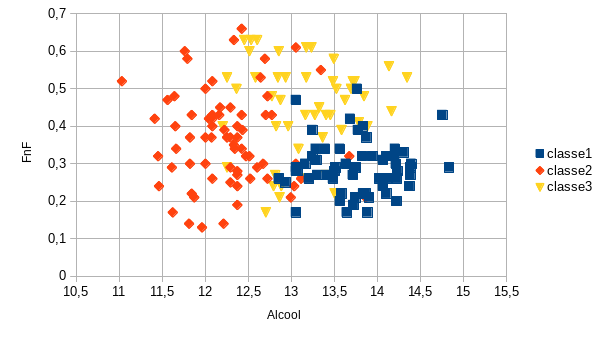
\includegraphics[scale=0.9]{figs/grafico_wine_alcool_FnF.png}
        \caption{Gráfico da disposição de elementos da Base Wine entre os eixos \textbf{FnF} e \textbf{Alcool}} \label{fig:grafico_wine_alcool_FnF}
\end{figure}

% Em uma análise do gráfico da figura \ref{fig:grafico_wine_alcool_FnF}, mesmo observando em uma pespectiva de duas variáveis, é possível visualizar o comportamento da base Wine quanto a disposição de seus dados, e através dos rótulos  sugeridos de pelo Naive Bayes pode-se constatar suas representações nos grupos, bem como também visualizar seus erros. e.g., quando um especialista verificar um determinado dado que possui no atributo alcool o valor 12.1, e este conhece os rótulos sugeridos pelo Naive Bayes, logo o especialista atribui que esse dado pertence ao grupo de vinho tipo 2. Esse exemplo pode ser constatado  com o gráfico da figura \ref{fig:grafico_wine_alcool_FnF}, pois ao confirmar o valor 12.1 no eixo X (alcool) percebe-se que este está junto a distribuição do grupo 2 conforme figura.

Em uma análise do gráfico da figura \ref{fig:grafico_wine_alcool_FnF}, mesmo observando em uma perspectiva de duas variáveis, é possível visualizar distribuição da base Wine  e, através dos rótulos sugeridos pelo Naive Bayes, pode-se constatar suas representações nos grupos, bem como também visualizar seus erros, \textit{e.g.}, quando um especialista verificar um determinado dado que possui no atributo \textbf{alcool}, o valor 12.1, e conhece os rótulos sugeridos pelo Naive Bayes, logo ele atribui que esse dado pertence ao grupo de vinho tipo 2. Esse exemplo pode ser constatado com o gráfico da figura \ref{fig:grafico_wine_alcool_FnF}, pois, ao confirmar o valor 12.1 no eixo X (\textbf{alcool}), percebe-se visualmente que este está junto à distribuição do grupo 2, conforme figura. 

A mesma figura também pode ser utilizada para explicar os rótulos sugeridos pelo KNN, que teve, em comparação com CART, melhor acurácia na rotulação do \textit{cluster} 1 e igual ao \textit{cluster} 3. Com rótulo do KNN ${r_{c_1}}$ $=\{(FnF, [ 0.13 \sim  0.306667  ] ) \} $, e através da figura \ref{fig:grafico_wine_alcool_FnF}, percebe-se que a faixa coberta pelo rótulo aponta para os dados do grupo 1 (classe 1 do gráfico). Da mesma forma acontece com o rótulo ${r_{c_3}=}$ ${\{ (FnF, ] 0.483333 \sim  0.66 ])\} }$, no qual valores do atributo \textbf{FnF} acima de 0.48 (vê gráfico figura \ref{fig:grafico_wine_alcool_FnF}) até 0.66 direcionam para o grupo 3 (classe 3 do gráfico), de modo a constatar que os rótulos conseguem representar os grupos dos tipos de vinho.

% Dos resultados encontrados pelo CART o rótulo do \textit{cluster} 1, dentre os três algoritmos foi o melhor, com acurácia de 66.2\%, já em relação a acurácia no \textit{cluster} 2 foi pior comparando aos outros dois algoritmos, no \textit{cluster} 3 já foi dito sobre a igualdade deste resultado com CART e teve a acurácia mais baixa do que o Naive Bayes.

Dos resultados encontrados pelo CART, o rótulo do \textit{cluster} 1, dentre os três algoritmos, foi o melhor, com acurácia de 66.2\%; já o cluster 2 em relação à acurácia, foi pior comparando-se aos outros dois algoritmos; no cluster 3, já foi dito sobre a igualdade deste resultado com CART, tendo a acurácia mais baixa do que o Naive Bayes. 

% 
% As tabelas \ref{tab:analise:wine:cluster1:matiz} e \ref{tab:analise:wine:cluster1:flavonoides} possuem uma amostra de registros do \textit{cluster} 1, em que é possível perceber quais os registros estão fazendo parte dos rótulos encontrados em cada algoritmo através das linhas em destaque. A tabela é formada pela primeira coluna indicando o número do registro na base de dados e em seguida os atributos. 
% 
% \begin{table}[!ht]
% \centering
% \caption{Amostra do \textit{cluster} 1 da base dados Wine, ordenados pelo atributo \textbf{matiz}}
% \label{tab:analise:wine:cluster1:matiz}
% \scalebox{0.8}{
% \small\addtolength{\tabcolsep}{-2pt}
% \begin{tabular}{|c|c|c|c|c|c|c|c|c|c|c|c|c|c|}
% \hline 
%  n. & álcool & AM & cinza & AC & magnésio & TF & flavonoides & FnF & proantocianidinas & IC & matiz & OD & prolina \\ \hline
%   
% 1 & 13,24 & 3,98 & 2,29 & 17,5 & 103 & 2,64 & 2,63 & 0,32 & 1,66 & 4,36 & 0,82 & 3 & 680\\ \hline
% 2 & 14,37 & 1,95 & 2,5 & 16,8 & 113 & 3,85 & 3,49 & 0,24 & 2,18 & 7,8 & 0,86 & 3,45 & 1480\\ \hline
% 3 & 14,21 & 4,04 & 2,44 & 18,9 & 111 & 2,85 & 2,65 & 0,3 & 1,25 & 5,24 & 0,87 & 3,33 & 1080\\ \hline
% 4 & 13,05 & 1,77 & 2,1 & 17 & 107 & 3 & 3 & 0,28 & 2,03 & 5,04 & 0,88 & 3,35 & 885\\ \hline
% 5 & 13,88 & 1,89 & 2,59 & 15 & 101 & 3,25 & 3,56 & 0,17 & 1,7 & 5,43 & 0,88 & 3,56 & 1095\\ \hline
% 6 & 14,22 & 3,99 & 2,51 & 13,2 & 128 & 3 & 3,04 & 0,2 & 2,08 & 5,1 & 0,89 & 3,53 & 760\\ \hline
% 7 & 13,72 & 1,43 & 2,5 & 16,7 & 108 & 3,4 & 3,67 & 0,19 & 2,04 & 6,8 & 0,89 & 2,87 & 1285\\ \hline
%  \rowcolor[HTML]{EFEFEF} 
% 8 & 13,41 & 3,84 & 2,12 & 18,8 & 90 & 2,45 & 2,68 & 0,27 & 1,48 & 4,28 & 0,91 & 3 & 1035\\ \hline
%  \rowcolor[HTML]{EFEFEF} 
% 9 & 13,9 & 1,68 & 2,12 & 16 & 101 & 3,1 & 3,39 & 0,21 & 2,14 & 6,1 & 0,91 & 3,33 & 985\\ \hline
% ... & ... & ... & ... & ... & ... & ... & ... & ... & ... & ... & ...& ... & ... \\ \hline
%  \rowcolor[HTML]{EFEFEF} 
% 58 & 14,75 & 1,73 & 2,39 & 11,4 & 91 & 3,1 & 3,69 & 0,43 & 2,81 & 5,4 & 1,25 & 2,73 & 1150\\ \hline
%  \rowcolor[HTML]{EFEFEF} 
% 59 & 13,63 & 1,81 & 2,7 & 17,2 & 112 & 2,85 & 2,91 & 0,3 & 1,46 & 7,3 & 1,28 & 2,88 & 1310\\ \hline
%   \end{tabular}}
%   \end{table}
%   
%   \begin{table}[!ht]
% \centering
% \caption{Amostra do \textit{cluster} 1 da base dados Wine, ordenados pelo atributo \textbf{flavonoides}}
% \label{tab:analise:wine:cluster1:flavonoides}
%   \scalebox{0.8}{
%   \small\addtolength{\tabcolsep}{-2pt}
%   \begin{tabular}{|c|c|c|c|c|c|c|c|c|c|c|c|c|c|}
%    
% \hline
% n. & álcool & AM & cinza & AC & magnésio & TF & flavonoides & FnF & proantocianidinas & IC & matiz & OD & prolina \\ \hline
%  \rowcolor[HTML]{EFEFEF} 
% 1 & 13,3 & 1,72 & 2,14 & 17 & 94 & 2,4 & 2,19 & 0,27 & 1,35 & 3,95 & 1,02 & 2,77 & 1285 \\ \hline
%  \rowcolor[HTML]{EFEFEF} 
% 2 & 14,02 & 1,68 & 2,21 & 16 & 96 & 2,65 & 2,33 & 0,26 & 1,98 & 4,7 & 1,04 & 3,59 & 1035 \\ \hline
%  \rowcolor[HTML]{EFEFEF} 
% 3 & 12,85 & 1,6 & 2,52 & 17,8 & 95 & 2,48 & 2,37 & 0,26 & 1,46 & 3,93 & 1,09 & 3,63 & 1015 \\ \hline
%  \rowcolor[HTML]{EFEFEF} 
% 4 & 12,93 & 3,8 & 2,65 & 18,6 & 102 & 2,41 & 2,41 & 0,25 & 1,98 & 4,5 & 1,03 & 3,52 & 770 \\ \hline
% ... & ... & ... & ... & ... & ... & ... & ... & ... & ... & ... & ...& ... & ... \\ \hline
%  \rowcolor[HTML]{EFEFEF} 
% 51 & 13,83 & 1,57 & 2,62 & 20 & 115 & 2,95 & 3,4 & 0,4 & 1,72 & 6,6 & 1,13 & 2,57 & 1130 \\ \hline
%  \rowcolor[HTML]{EFEFEF} 
% 52 & 14,37 & 1,95 & 2,5 & 16,8 & 113 & 3,85 & 3,49 & 0,24 & 2,18 & 7,8 & 0,86 & 3,45 & 1480 \\ \hline
%  
% 53 & 13,94 & 1,73 & 2,27 & 17,4 & 108 & 2,88 & 3,54 & 0,32 & 2,08 & 8,9 & 1,12 & 3,1 & 1260 \\ \hline
% 54 & 13,88 & 1,89 & 2,59 & 15 & 101 & 3,25 & 3,56 & 0,17 & 1,7 & 5,43 & 0,88 & 3,56 &  1095 \\ \hline
% 55 & 14,38 & 1,87 & 2,38 & 12 & 102 & 3,3 & 3,64 & 0,29 & 2,96 & 7,5 & 1,2 & 3 & 1547 \\ \hline
% 56 & 13,72 & 1,43 & 2,5 & 16,7 & 108 & 3,4 & 3,67 & 0,19 & 2,04 & 6,8 & 0,89 & 2,87 & 1285 \\ \hline
% 57 & 14,75 & 1,73 & 2,39 & 11,4 & 91 & 3,1 & 3,69 & 0,43 & 2,81 & 5,4 & 1,25 & 2,73 & 1150 \\ \hline
% 58 & 13,82 & 1,75 & 2,42 & 14 & 111 & 3,88 & 3,74 & 0,32 & 1,87 & 7,05 & 1,01 & 3,26 & 1190\\ \hline
% 59 & 14,19 & 1,59 & 2,48 & 16,5 & 108 & 3,3 & 3,93 & 0,32 & 1,86 & 8,7 & 1,23 & 2,82 & 1680\\ \hline
% \end{tabular}}
% \end{table}


%Comparando-se os rótulos de todos os três algoritmos, percebe-se que o número de erros encontrados pelos três algoritmos são os mesmos, porém no \textit{cluster} 1 do Naive Bayes e CART, o atributo rótulo é diferente do KNN, e mesmo com o número de erros e acurácias iguais, isso não implica afirmar que os registros representados por um rótulo,  ${r_{c_1}=\{ (matiz, ] 0.890000 \sim  1.3000])\} }$ tabela \ref{tab:rot:wine:nb} e \ref{tab:rot:wine:cart}, são os mesmos representados no outro rótulo encontrado pelo algoritmo KNN ${r_{c_1}=\{ (flavonoides, ] 1.920000 \sim  3.500000])\} }$, e a única forma de verificar essa situação é analisar diretamente a base e identificar os registros. Por esse motivo, as tabelas \ref{tab:analise:wine:cluster1:matiz} e \ref{tab:analise:wine:cluster1:flavonoides} são amostras com os registros da base e com elas é possível perceber quais os registros estão participando do rótulo, pois todos os registros destacados fazem parte dele e os que não estão marcados são os registros que não são representados pelo rótulo. 



%Analisando-se as tabelas, verifica-se que a única coincidência está nas linhas 5 e 7 da tabela  \ref{tab:analise:wine:cluster1:matiz}, pois são as mesmas da tabela \ref{tab:analise:wine:cluster1:flavonoides}, linhas 55 e 56, e esses registros coincidem por também não serem representados pelos rótulos. Assim, ainda que os rótulos de clusters possuam como resposta de algoritmos diferentes número de erros e acurácias iguais, não significa dizer que eles estão representando os mesmos registros, porém, os rótulos têm o mesmo poder de representatividade do \textit{cluster}, por possuírem números de erros iguais, podendo o analista optar por qualquer algoritmo.

\section{Discussões}


A figura  \ref{fig:acuracia_media_algoritmos} mostra um gráfico geral da acurácia média de todos os rótulos encontrados na aplicação dos algoritmos nas bases de dados. O eixo Y corresponde à porcentagem de acurácia média alcançada de um algoritmo e o eixo X está dividido nos \textit{clusters} e a qual base de dados eles pertencem. Essa acurácia é aferida a partir das acurácias parciais do(s) atributo(s) que faz(em) parte do rótulo e, caso o rótulo possua mais de um atributo, é calculada uma média das acurácias parciais. 

\begin{figure}[h!]
        \centering
        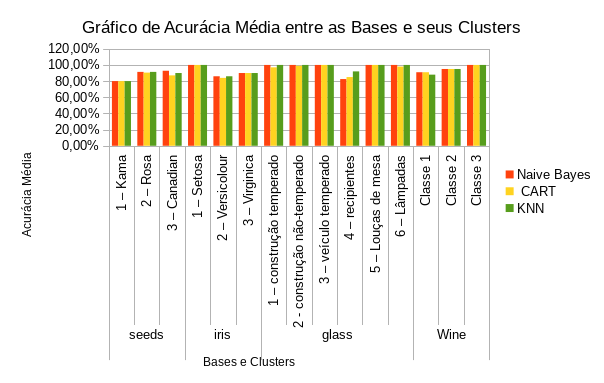
\includegraphics[scale=0.9]{figs/grafico_acuracia_media_algoritmos.png}
        \caption{Acurácia média entre os clusters de todas as bases testadas com os algoritmos: Naive Bayes, CART e KNN} \label{fig:acuracia_media_algoritmos}
\end{figure}

Foram testadas quatro bases de dados e dentre elas a base Wine, uma base de resultado de análises químicas com 178 amostras dividida em três tipos de vinhos. Foi a única a possuir algumas acurácias de rótulos por clusters abaixo de 60\%, já as demais bases, Seeds, Iris e Glass, tiveram suas acurácias dos rótulos por clusters acima de 70\%, \textit{e.g.}, se um rótulo conseguir representar 70\% de uma amostra de quinhento registros, isso implica que o rótulo consegue representar trezentos e cinquenta registros do quinhentos, considerando assim um rótulo satisfatório nessa amostra.

%É possível verificar no gráfico da figura \ref{fig:acuracia_media_algoritmos} algoritmo



Outra pesquisa \cite{Lopes2016} também realizou testes com essas mesmas bases para realizar rotulação de dados, mas, diferente deste trabalho, o autor citado não considerou a classificação das bases, ou seja,  não utilizou os grupos já designados na origem das bases, e realizou  uma nova classificação através de um algoritmo não-supervisionado,\textit{ K-means}, e só assim aplicou um algoritmo de aprendizado  de máquina supervisionado (RNAs). Para esta pesquisa poder realizar uma comparação entre os resultados, é necessário recriar os grupos e em seguida aplicar os algoritmos supervisionados para obter os rótulo. 

A rotulação de grupos tem dependência direta dos registros pertencentes ao grupo e qualquer alteração destes registros implica em uma alteração nos resultados dos rótulos. Dessa maneira foram realizados testes para recriar os mesmos grupos que \citeonline{Lopes2016}, mas mesmo utilizando as mesmas técnicas as tentativas não lograram êxito em fazer grupos idênticos, pois mesmo configurando o número de grupos a ser encontrado pelo algoritmo, ao executá-lo, os resultados retornam grupos diferentes um do outro, de forma que uma comparação com grupos diferentes não retrataria uma comparação justa, pois os dados testados não seriam os mesmos\footnote{Resultados dos testes comparativos no Apêndice \ref{apendice:1}}.

Para conseguir as acurácias dos rótulos deste trabalho foi necessária a utilização de bases de dados com classes definidas, pois a partir dos rótulos encontrados é possível saber se os elementos das amostras eram representados por eles, entretanto, este estudo tem o objetivo de identificar grupos que não tem classes conhecidas e a partir da rotulação conseguir representar esses grupos. Portanto, o envolvimento de bases classificadas faz parte desse estudo somente para comprovação de resultados, e para mostrar a  viabilidade dos rótulos através das acurácias e apresentando que é possível rotular grupos de dados.








\chapter{Conclusões, Trabalhos Futuros}\label{cap:conclusao} 

Neste capítulo serão apresentadas as considerações finais da dissertação, bem como a apresentação dos benefícios da pesquisa realizada, que teve como base a rotulação de algoritmos com vistas a analisar o seu comportamento considerando algumas bases de dados consolidadas. Também serão apresentadas sugestões para continuidade deste trabalho já efetuado.

\section{Conclusão}\label{cond}

O presente trabalho dedicou-se a estudar a aplicabilidade de algoritmos supervisionados com bases de dados distintas, as bases utilizadas foram: Seeds, Iris, Glass e Wine, com a finalidade de definir a tupla atributo/valor de maior importância nos \textit{clusters}, determinando a sua rotulação. A formação do referido problema nasceu de outra pesquisa já concluída \cite{Lopes2016}, entretanto, teve como diferencial a realização de rotulação de grupos de dados a partir de algoritmos supervisionados não testados, Naive Bayes, Classification and Regression Trees - CART e K-Nearest Neighbor - KNN, assim, ao final foi possível demonstrar o comparativo de resultados.


As análises foram feitas a partir das bases de dados mencionadas acima, e o comportamento ao aplicar cada algoritmo nas bases e encontrar os rótulos foram satisfatórios. A avalição da qualidade destes rótulos foi feita da seguinte forma: inicialmente, escolheu-se as bases de dados já classificadas; feito isso foi possível saber quantas amostras pertencem a determinado grupo; em seguida, foi realizado um comparativo dos resultados dos rótulos através dos erros encontrados, e nos grupos com as amostras originais das bases de dados, desta forma foi possível mensurar a acurácia de cada rótulo. 
%Então, para avaliar a qualidade do rótulo quando existe um empate no número de erros

%Existe duas situações que podem acontecer para escolha do rótuloPara a escolha do melhor rótulo quando existir um empate entre os algoritmos

O funcionamento dos algoritmos foram também  marcados pelas bases utilizadas, a base de dados 1 - Seeds, é uma base de dados balanceada, que neste caso, possui um número de exemplos iguais para as três classes (70 elementos cada classe), destacando-se que a mesma obteve rótulos diferentes entre os três algoritmos, sua acurácia foi alta, considerando que a menor acurácia parcial de grupo chegou a 80\%, e a maior, aproximadamente 94\%. A base de dados 2 - Iris, tiveram rótulos idênticos em dois algoritmos, Naive Bayes e KNN, e no CART a diferença ficou somente no \textit{cluster} 2 ( \textit{Iris-versicolor}), que deu maior importância para o largura da pétala (\textit{petalwidth}) ao invés do comprimento da pétala (\textit{petallength}) encontrada nos outros dois algoritmos, porém, a escolha do \textit{petalwidth}, pelo CART, ocasionou um número de erros um pouco maior em comparação com os outros dois algoritmos (Naive Bayes e KNN). 

Na base de dados 3 - Glass, os rótulos foram bastantes satisfatórios ao  analisar as acurácias dos algoritmos chegando em vários \textit{clusters} a acurácias de 100\%, contudo, os rótulos do Naive Bayes e CART em específico no \textit{cluster} 4 (grupo recipientes), mesmo tendo poucos erros a acurácia chegou em 77\% em alguns atributos rótulos. Vale ressaltar que essa base não é classificada como uma base balanceada e no grupo, recipientes, conta com somente treze elementos. Já na base de dados 4 - Wine, possui um total de 178 (cento e setenta e oito) registros, de forma balanceada, pois possui um número mínimo de 48 (quarenta e oito) elementos no grupo. Nesta base os rótulos foram bastantes semelhantes, e diferenciados apenas no \textit{cluster} 1 do KNN que obteve um atributo rótulo diferentes dos outros algoritmos, porém o número de erros de todos os rótulos foram iguais afirmando que os três possuem o mesmo poder de representar os clusters com seus rótulos.


Outro ponto que merece destaque é a tomada de decisão através dos rótulos encontrados neste trabalho, isto é, acurácias altas resultam em boa confiabilidade dos rótulos, portanto quando um especialista da área verificar um rótulo de um grupo, este será capaz de perceber o que é importante para o grupo, podendo fazer uma tomada de decisão mais eficiente a partir destes resultados.

Assim, diante do problema de rotulação, que visa encontrar informações relevantes em grupos de dados ao ponto de identificar esses grupos, e considerando que \citeonline{Lopes2016} utilizou algoritmo supervisionado com paradigma conexionista (Redes Neurais) neste problema, esta pesquisa apresentou aplicação de novos algoritmos com paradigmas diferentes, ainda não testados, mostrando a viabilidade do método de rotulação de dados com algoritmos de aprendizado supervisionados, e comparando os resultados através das acurácias dos rótulos encontradas em cada \textit{cluster}.


%É importante destacar que este trabalho buscou analisar a aplicação de algoritmos com paradigmas diferentes, a partir das bases citadas, portanto, foi possível conhecer a acurácia de cada algoritmo testado, demonstrando que todos possuem alto grau de confiança, já que variaram de 82.5\% a 100\% na acurácia média, métrica esta calculada de acordo com os grupos extraído da própria fonte\footnote{UCI - Machine Learning Repository. http://archive.ics.uci.edu/ml/}, e assim confirmar que é possível realizar rotulação de dados. 

%Assim, uma análise desse trabalho pode ser descrita da seguinte forma: i) De acordo com a proposta de encontrar rótulos com algoritmos não antes testados em bases de dados já utilizadas em outros trabalhos, foi fielmente cumprido e 

%a análise aqui apresentada é eficiente perante os resultados, porém foi detectado que há  discretização e o número de faixas é essencial para  os resultado dos algoritmos na produção dos rótulos. A técnica utilizada nesta pesquisa segue a característica da aprendizagem supervisionada, ou seja, atributos de entrada se correlacionam para gerar uma saída desejável através de um atributo classe. Então, se os dados contém um grande número de características independentes com alta correlação com a classe, isso ajuda no aprendizado, contudo, se o combinação entre as variáveis é muito complexo, acaba dificultando o aprendizado dessa relação. Isto posto, percebe-se que a discretização tem influência direta nos rótulos encontrados, portanto, se um registro em um determinado método de discretização pertence a uma faixa de valor ao modificar esse método poderá também o registro mudar sua faixa, então, o que antes era rótulo pode não ser mais. 



%\section*{Trabalhos Futuros}
%\addcontentsline{toc}{chapter}{Trabalhos Futuros}
\section{Trabalhos Futuros}\label{cap:fut}



Espera-se realizar estudos mais profundos nos métodos de discretização, pois estes, tem influência comprovada na geração dos rótulos nos grupos de dados, e também no número de faixas, por está diretamente ligado aos métodos de discretização. A melhor discretização e o melhor número de faixas a ser utilizado está relacionado aos valores das bases de dados utilizada, e portanto  será necessário um estudo aprofundado para comparar os  resultados com os deste trabalho.



% ----------------------------------------------------------
% ELEMENTOS PÓS-TEXTUAIS (Referências, Glossário, Apêndices)
% ----------------------------------------------------------
\postextual

% Referências bibliográficas

\bibliography{mestradobib}


% Glossário (Consulte o manual)
%\glossary

% Apêndices
 % ----------------------------------------------------------
% Apêndices
% ----------------------------------------------------------

% ---
% Inicia os apêndices
% ---
\begin{apendicesenv}

% Imprime uma página indicando o início dos apêndices
\partapendices

% ----------------------------------------------------------
\chapter{Outros resultados de Rotulação }
% ----------------------------------------------------------
\label{apendice:1}

Através da pesquisa de \citeonline{Lopes2016} que apresentou um modelo de rotulação de dados, ao qual através de um algoritmo não-supervisionado gera grupos de uma determinada base de dados, e logo após, é aplicado um outro algoritmo com aprendizagem supervisionada nesses grupos para detectar um rótulo para esses grupos. Mediante isso foram realizados testes com as mesmas bases de dados com finalidade de comparar os resultados, mas os testes não foram satisfatórios, embora algumas bases sejam iguais houve diferença entre os clusters criados. Foram realizados o uso das mesmas técnicas do autor citado acima, todavia não foi o bastante para que os grupos fossem os mesmos, ou seja, grupos definidos não são iguais e por consequência os teste ficaram incompatíveis.

Segue nas tabelas abaixo o comparativo do trabalho do \cite{Lopes2016} com os testes realizados nos clusters recriados das bases: Seeds, Iris e Glass, com o trabalho 

\begin{table}[H]
\centering
\caption{Rotulação de Dados utilizando a base de dados Seeds.}
\subfloat[Naive Bayes]{
\label{tab:comparativo:seeds:nb}
\scalebox{0.8}{
 \small\addtolength{\tabcolsep}{-2pt} 
\begin{tabular}{|c|c|c|c|c|}
\hline
\rowcolor[HTML]{EFEFEF} 
\hline
Cluster             & Num\_Elem              & Atributo     & Erro (qtd) & Erro (\%) \\ \hline
1                   &    72                  &  asymetry    & 25   & 34.7\\ \hline
                    &                        & Lkernel        & 1  & 1.64\\  
\multirow{-2}{*}{2} &   \multirow{-2}{*}{61} & lkgroove        & 5  & 8.19\\ \hline 
3                   &    77                  & perimetro       & 10  & 12.98\\ \hline
\multicolumn{3}{|c|}{Total}                             & 41   &\\ \hline
\end{tabular}
} %fim scalebox
} % fim subfloat
\subfloat[CART]{
\label{tab:comparativo:seeds:cart}
\scalebox{0.8}{%
 \small\addtolength{\tabcolsep}{-2pt} 
\begin{tabular}{|c|c|c|c|c|}
\hline
\rowcolor[HTML]{EFEFEF} 
\hline
Cluster             & Num\_Elem              & Atributo     & Erro (qtd) & Erro (\%)\\ \hline
1                   &    72                  &  perimetro    & 14  & 19.44 \\ \hline
2                   &   61                   & perimetro     & 0  & 0\\ \hline 
3                   &    77                  & perimetro      & 10  & 12.98\\ \hline
\multicolumn{3}{|c|}{Total}                             & 24  & \\ \hline
\end{tabular}
} %fim scalebox
} % fim subfloat

\subfloat[KNN]{
\label{tab:comparativo:seeds:knn}
\scalebox{0.8}{%
 \small\addtolength{\tabcolsep}{-2pt} 
\begin{tabular}{|c|c|c|c|c|}
\hline
\rowcolor[HTML]{EFEFEF} 
\hline
Cluster             & Num\_Elem              & Atributo     & Erro (qtd) & Erro (\%)\\ \hline
1                   &    72                  &  perimetro    & 14   & 19.44\\ \hline
2                   &   61                   & lkgroove     & 5  & 8.19\\ \hline 
3                   &    77                  & perimetro      & 10 &  12.98\\ \hline
\multicolumn{3}{|c|}{Total}                             & 29  & \\ \hline
\end{tabular}
} %fim scalebox
} % fim subfloat

\subfloat[Resultado de \citeonline{Lopes2016}]{
\label{tab:comparativo:seeds:lopes}
\scalebox{1}{%
 \small\addtolength{\tabcolsep}{-2pt} 
\begin{tabular}{|c|c|c|c|c|}
\hline
\rowcolor[HTML]{EFEFEF} 
\hline
Cluster             & Num\_Elem              & Atributo     & Erro (qtd) & Erro (\%) \\ \hline
                   &                       &  area    & 8   &  11.95 \\
\multirow{-2}{*}{1} &   \multirow{-2}{*}{67} & perimetro        & 9  & 13.64\\  \hline
                    &                        & area        & 12  & 14.64\\
\multirow{-2}{*}{2} &   \multirow{-2}{*}{82} & perimetro        & 10  & 12.2\\ \hline 
                    &                      & perimetro       & 0  & 0\\ 
                    &                        & wkernel        & 3  & 4.92\\  
                    &                      & lkernel       & 1  & 1.64\\ 
\multirow{-4}{*}{3} &   \multirow{-4}{*}{61} & area        & 0  & 0\\  \hline
\multicolumn{3}{|c|}{Total}                             & 43   &\\ \hline
\end{tabular}
} %fim scalebox
} % fim subfloat
\end{table}



\begin{table}[H]
\centering
\caption{Rotulação de Dados utilizando a base de dados Iris.}
\subfloat[Naive Bayes]{
\label{tab:comparativo:iris:nb}
\scalebox{1}{
 \small\addtolength{\tabcolsep}{-2pt} 
\begin{tabular}{|c|c|c|c|c|}
\hline
\rowcolor[HTML]{EFEFEF} 
\hline
Cluster             & Num\_Elem              & Atributo     & Erro (qtd) & Erro (\%) \\ \hline
                    &                        & sepallength        & 10  & 26.3\\  
\multirow{-2}{*}{1} &   \multirow{-2}{*}{38} & petalwidth        & 4  & 10.5\\ \hline 
2                   &    62                  & petalwidth       & 19  & 30.6\\ \hline
3                   &    50                  & petalwidth       & 0  & 0\\ \hline
\multicolumn{3}{|c|}{Total}                             & 33   &\\ \hline
\end{tabular}
} %fim scalebox
} % fim subfloat

\subfloat[CART]{
\label{tab:comparativo:iris:cart}
\scalebox{1}{%
 \small\addtolength{\tabcolsep}{-2pt} 
\begin{tabular}{|c|c|c|c|c|}
\hline
\rowcolor[HTML]{EFEFEF} 
\hline
Cluster             & Num\_Elem              & Atributo     & Erro (qtd) & Erro (\%)\\ \hline
1                   &    38                  &  petalwidth    & 4  & 10.5 \\ \hline
2                   &   62                   & petalwidth     & 19  & 30.6\\ \hline 
3                   &    50                  & petalwidth      & 0  & 0\\ \hline
\multicolumn{3}{|c|}{Total}                             & 23  & \\ \hline
\end{tabular}
} %fim scalebox
} % fim subfloat

\subfloat[KNN]{
\label{tab:comparativo:iris:knn}
\scalebox{1}{%
 \small\addtolength{\tabcolsep}{-2pt} 
\begin{tabular}{|c|c|c|c|c|}
\hline
\rowcolor[HTML]{EFEFEF} 
\hline
Cluster             & Num\_Elem              & Atributo     & Erro (qtd) & Erro (\%)\\ \hline
1                   &    38                  &  sepallength   & 10   & 26.3\\ \hline
2                   &   62                   & petalwidth     & 19  & 30.6\\ \hline 
3                   &    50                  & petalwidth      & 0 &  0\\ \hline
\multicolumn{3}{|c|}{Total}                             & 29  & \\ \hline
\end{tabular}
} %fim scalebox
} % fim subfloat

\subfloat[Resultado de \citeonline{Lopes2016}]{
\label{tab:comparativo:iris:lopes}
\scalebox{1}{%
 \small\addtolength{\tabcolsep}{-2pt} 
\begin{tabular}{|c|c|c|c|c|}
\hline
\rowcolor[HTML]{EFEFEF} 
\hline
Cluster             & Num\_Elem              & Atributo     & Erro (qtd)& Erro (\%) \\ \hline
                   &                       &  petalwidth    & 0   & 0 \\
\multirow{-2}{*}{1} &   \multirow{-2}{*}{50} & petallength   & 0  & 0\\  \hline
                   2 &          62              & petallength   & 6  & 9.68\\ \hline
                     &                        & petallength        & 3  & 7.9\\
\multirow{-2}{*}{3} &   \multirow{-2}{*}{38} & petalwidth        & 2  & 5.27 \\ \hline 
\multicolumn{3}{|c|}{Total}                             & 11   &\\ \hline
\end{tabular}
} %fim scalebox
} % fim subfloat
\end{table}
\FloatBarrier

\begin{table}[H]
\centering
\caption{Rotulação de Dados utilizando a base de dados Glass}
\subfloat[Naive Bayes]{
\label{tab:comparativo:glass:nb}
\scalebox{0.8}{
 \small\addtolength{\tabcolsep}{-2pt} 
\begin{tabular}{|c|c|c|c|c|}
\hline
\rowcolor[HTML]{EFEFEF} 
\hline
Cluster             & Num\_Elem              & Atributo     & Erro (qtd) & Erro (\%)\\ \hline
                  &                    & Ba  & 1 & 1,45\\
\multirow{-2}{*}{1} & \multirow{-2}{*}{69} & Fe  & 11 & 15,94\\ \hline
 &  & Mg  & 2 & 50,00\\
 &  & K   & 2 & 50,00\\
 &  & Ba  & 2 & 50,00\\
\multirow{-3}{*}{2} & \multirow{-2}{*}{4}& Fe  & 0 & 0,00\\ \hline
 &  & RI  & 11 & 35,48\\
 &  & Mg  & 2 & 6,45\\
 &  & Al  & 14 & 45,16\\
 &  & Si  & 6 & 19,35\\
 &  & K   & 1 & 3,23\\
 &  & Ba  & 12 & 38,71\\
\multirow{-7}{*}{3} & \multirow{-7}{*}{31} & Fe  & 0 & 0,00\\ \hline
 &  & RI  & 6 & 16,67\\
 &  & Na  & 11 & 30,56\\
 &  & Mg  & 12 & 33,33\\
 &  & Al  & 17 & 47,22\\
 &  & Si  & 6 & 16,67\\
 &  & K   & 0 & 0,00\\
 &  & Ca  & 1 & 2,78\\
 &  & Ba  & 1 & 2,78\\
\multirow{-9}{*}{4} & \multirow{-9}{*}{36}& Fe  & 8 & 22,22\\ \hline
 &  & Mg  & 2 & 12,50\\
 &  & Al  & 6 & 37,50\\
 &  & Ba  & 1 & 6,25\\
\multirow{-4}{*}{5} & \multirow{-4}{*}{16} & Fe  & 4 & 25,00\\ \hline
 &  & Si  & 6 & 10,34\\
 &  & K   & 0 & 0,00\\
 &  & Ba  & 0 & 0,00\\
\multirow{-4}{*}{6} & \multirow{-4}{*}{58} &Fe& 20 & 34,48\\ \hline
\multicolumn{3}{|c|}{Total}                             & 165  & \\ \hline
\end{tabular}
} %fim scalebox
} % fim subfloat
\subfloat[CART]{
\label{tab:comparativo:glass:cart}
\scalebox{0.8}{%
 \small\addtolength{\tabcolsep}{-2pt} 
\begin{tabular}{|c|c|c|c|c|}
\hline
\rowcolor[HTML]{EFEFEF} 
\hline
Cluster             & Num\_Elem              & Atributo     & Erro (qtd) & Erro (\%)\\ \hline
 &  & Ba  & 1 & 1,45\\
\multirow{-2}{*}{1} & \multirow{-2}{*}{69} & Fe  & 17 & 24,64\\  \hline
 &  & Mg  & 1 & 25,00\\
 &  & K   & 0 & 0,00\\
 &  & Ba  & 2 & 50,00\\
\multirow{-3}{*}{2} & \multirow{-3}{*}{4} & Fe  & 0 & 0,00\\ \hline
 &  & Mg  & 0 & 0,00\\
 &  & K   & 3 & 9,68\\
&  & Ba  & 22 & 70,97\\
\multirow{-4}{*}{3} & \multirow{-4}{*}{31} & Fe  & 0 & 0,00\\ \hline
 &  & RI  & 7 & 19,44\\
 &  & Na  & 19 & 52,78\\
 &  & Mg  & 20 & 55,56\\
 &  & Al  & 16 & 44,44\\
 &  & Si  & 8 & 22,22\\
 &  & K   & 15 & 41,67\\
 &  & Ca  & 14 & 38,89\\
 &  & Ba  & 2 & 5,56\\
\multirow{-9}{*}{4} & \multirow{-9}{*}{36} & Fe  & 10 & 27,78\\ \hline
 &  & Mg  & 0 & 0,00\\
 &  & Al  & 10 & 62,50\\
 &  & Ba  & 1 & 6,25\\
\multirow{-4}{*}{5} & \multirow{-4}{*}{16} & Fe  & 5 & 31,25\\ \hline
 &  & K   & 12 & 20,69\\
 &  & Ba  & 0 & 0,00\\
\multirow{-3}{*}{6} & \multirow{-3}{*}{58} & Fe  & 23 & 39,66\\ \hline

\multicolumn{3}{|c|}{Total}                             & 208  & \\ \hline
\end{tabular}
} %fim scalebox
} % fim subfloat

\subfloat[KNN]{
\label{tab:comparativo:glass:knn}
\scalebox{0.8}{%
 \small\addtolength{\tabcolsep}{-2pt} 
\begin{tabular}{|c|c|c|c|c|}
\hline
\rowcolor[HTML]{EFEFEF} 
\hline
Cluster             & Num\_Elem              & Atributo     & Erro (qtd) & Erro (\%)\\ \hline
 &  & Ba  & 1 & 1,45\\
\multirow{-2}{*}{1} & \multirow{-2}{*}{69} & Fe  & 11 & 15,94\\ \hline
 &  & Mg  & 2 & 50,00\\
 &  & K   & 2 & 50,00\\
 &  & Ba  & 2 & 50,00\\
\multirow{-4}{*}{2} & \multirow{-4}{*}{4} & Fe  & 0 & 0,00\\ \hline
 &  & Mg  & 2 & 6,45\\
 &  & Al  & 14 & 45,16\\
 &  & K   & 1 & 3,23\\
 &  & Ba  & 12 & 38,71\\
\multirow{-5}{*}{3} & \multirow{-5}{*}{31} & Fe  & 0 & 0,00\\ \hline
 &  & RI  & 6 & 16,67\\
 &  & Na  & 11 & 30,56\\
 &  & Al  & 17 & 47,22\\
 &  & Si  & 6 & 16,67\\
 &  & K   & 0 & 0,00\\
 &  & Ca  & 1 & 2,78\\
 &  & Ba  & 1 & 2,78\\
\multirow{-8}{*}{1} & \multirow{-8}{*}{36} & Fe  & 8 & 22,22\\ \hline
 &  & Mg  & 2 & 12,50\\
 &  & Ba  & 1 & 6,25\\
\multirow{-3}{*}{5} & \multirow{-3}{*}{16} & Fe  & 4 & 25,00\\ \hline
 &  & K   & 0 & 0,00\\
 &  & Ba  & 0 & 0,00\\
\multirow{-3}{*}{6} & \multirow{-3}{*}{58} & Fe  & 20 & 34,48\\ \hline
\multicolumn{3}{|c|}{Total}                             &  124 & \\ \hline
\end{tabular}
} %fim scalebox
} % fim subfloat
\subfloat[Resultado de \citeonline{Lopes2016}]{
\label{tab:comparativo:glass:lopes}
\scalebox{0.8}{%
 \small\addtolength{\tabcolsep}{-2pt} 
\begin{tabular}{|c|c|c|c|c|}
\hline
\rowcolor[HTML]{EFEFEF} 
\hline
Cluster             & Num\_Elem              & Atributo     & Erro (qtd) & Erro (\%) \\ \hline
 &  & Ba & 0 & 0\\
 &  & K & 0 & 0\\
 &  & Si & 2 & 2,71\\
\multirow{-2}{*}{1} &   \multirow{-2}{*}{74}& Na & 3 & 4,06\\ \hline
  &  & Fe & 0 & 0\\
 \multirow{-2}{*}{2} &   \multirow{-2}{*}{5} & Ca & 0 & 0\\ \hline
  &  & K & 0 & 0\\
 \multirow{-2}{*}{3} &   \multirow{-2}{*}{19} & Ba & 1 & 5,27 \\ \hline
  &   & K & 0 & 0\\
 &  &  Ba & 1 & 3,13\\
\multirow{-3}{*}{4} &   \multirow{-3}{*}{32} & Ca & 1 & 3,13\\ \hline
 &  & Ba & 0 & 0\\
 &  & K & 0 & 0\\
 &  &  Na & 2 & 3,58\\
 &  & Al & 4 & 7,15\\
\multirow{-5}{*}{5} &   \multirow{-5}{*}{56}  & Mg & 6 & 10,72\\ \hline
  &  & Fe & 0 & 0\\
 \multirow{-2}{*}{6} &   \multirow{-2}{*}{28} & K & 1 & 3,58 \\ \hline
\multicolumn{3}{|c|}{Total}                             & 21   &\\ \hline
\end{tabular}
} %fim scalebox
} % fim subfloat
\end{table}

%\lipsum[50] % Texto qualquer. REMOVER!!

% ----------------------------------------------------------
\chapter{Características da Implementação}
% ----------------------------------------------------------
\label{apendice:2}
Utilizando como referência o  trabalho de  \cite{Lopes2016} foi utilizado como ferramenta de desenvolvimento o MATLAB\footnote{http://www.mathworks.com/products/matlab/ ; versão: R2016a(9.0.0.341360); 64-bit (glnxa64)}, uma poderosa ferramenta matemática e IDE de desenvolvimento com recursos de aprendizado de máquina em pacotes chamados de \textit{Statistics and Machine Learning Toolbox}. De acordo com a documentação do MATLAB\footnote{https://la.mathworks.com/help/stats/supervised-learning-machine-learning-workflow-and-algorithms.html?lang=en} a  tabela \ref{tab:matlab} exibe quais algoritmos são implementados pela Toolbox.



\begin{table}[H]
\centering
\caption{Informações retiradas da documentação do MATLAB v.2016a - Supervised Learning Workflow and Algorithms}
\label{tab:matlab}
\scalebox{0.6}{
\begin{tabular}{p{3cm}|p{4cm}|p{3cm}|p{5cm}|p{5cm}|p{4.5cm}}%p{65}|p{70}|p{100}|p{100}|p{100}|p{100}
\hline
\rowcolor[HTML]{EFEFEF}
Classificador & Suporta multi-classes & Suporta Preditor Categórico & Velocidade de Predição & Utilização de Memória & Interpretabilidade\\ \hline
Decision trees — fitctree & Yes & Yes & Fast & Small & Easy\\ \hline
Discriminant analysis — fitcdiscr & Yes & No & Fast & Small for linear, large for quadratic & Easy\\ \hline
SVM — fitcsvm & No. Combine multiple binary SVM classifiers using fitcecoc. & Yes & Medium for linear. Slow for others. & Medium for linear. All others: medium for multiclass, large for binary. & Easy for linear SVM. Hard for all other kernel types.\\ \hline
Naive Bayes — fitcnb & Yes & Yes & Medium for simple distributions. Slow for kernel distributions or high-dimensional data & Small for simple distributions. Medium for kernel distributions or high-dimensional data & Easy\\ \hline
Nearest neighbor — fitcknn & Yes & Yes & Slow for cubic. Medium for others. & Medium & Hard\\ \hline
Ensembles — fitensemble & Yes & Yes & Fast to medium depending on choice of algorithm & Low to high depending on choice of algorithm. & Hard\\ \hline
\end{tabular}}
\end{table}

Esta tabela exibe algoritmos de aprendizado  supervisionados e suas característica através de resultados  estudados de bases de dados com mais de 7000 observações e 50 classes.

Uma vez decidido pela utilização da \textit{toolbox} e suas característica expostas na tabela \ref{tab:matlab}, foi escolhida para este trabalho um algoritmo por paradigma; simbólico (árvore de decisão com CART), bayesiano (probabilístico Nave Bayes) e analogia ou baseado em instância (KNN). Alguns dos algoritmos mostrado na tabela não foram  utilizados, como:  Discriminant analysis pois é do mesmo tipo bayesiano e Ensembles funciona com várias outras implementações de regressões e classificações com pequenas nuances, e também não foi utilizado por sair do foco desta pesquisa.



\end{apendicesenv}
% ---


% Anexos
% % ----------------------------------------------------------
% Apêndices
% ----------------------------------------------------------

% ---
% Inicia os anexos
% ---
\begin{anexosenv}

% Imprime uma página indicando o início dos anexos
\partanexos

% ---
\chapter{Nome do Primeiro Anexo}
% ---
\lipsum[30] % Texto qualquer. REMOVER!!

% ---
\chapter{Nome de Outro Anexo}
% ---

\lipsum[32] % Texto qualquer. REMOVER!!

\end{anexosenv}

% Índice remissivo (Consultar manual)
%\phantompart
%\printindex

\end{document}
